%==================================================================
% PROPOSAL PENELITIAN METODOLOGI PENELITIAN — STANDAR FMIPA UNNES
% Mengacu pada template standar bimbingan Dr. Iqbal Kharisudin, M.Sc.
%==================================================================
\documentclass[12pt,a4paper]{article}

\usepackage[utf8]{inputenc}
\usepackage[T1]{fontenc}
\usepackage{amsmath,amssymb}
\usepackage{mathptmx}
\usepackage{graphicx}
\usepackage[a4paper,left=4cm,right=3cm,top=3cm,bottom=3cm]{geometry}
\usepackage{setspace}
\usepackage{booktabs}
\usepackage{array}
\usepackage{tabularx}
\usepackage{float}
\usepackage{caption}
\usepackage[round,authoryear]{natbib}
\setcitestyle{aysep={,},yysep={,},notesep={, }}
\usepackage{fancyhdr}
\usepackage[colorlinks=true,linktocpage=true,linkcolor=blue,citecolor=blue,urlcolor=blue]{hyperref}

\renewcommand{\contentsname}{DAFTAR ISI}
\renewcommand{\listfigurename}{DAFTAR GAMBAR}
\renewcommand{\listtablename}{DAFTAR TABEL}
\renewcommand{\figurename}{Gambar}
\renewcommand{\tablename}{Tabel}

\renewcommand{\thesection}{\Roman{section}}
\renewcommand{\thesubsection}{\arabic{section}.\arabic{subsection}}
\renewcommand{\thesubsubsection}{\arabic{section}.\arabic{subsection}.\arabic{subsubsection}}
\makeatletter
\@addtoreset{figure}{section}
\@addtoreset{table}{section}
\renewcommand{\thefigure}{\arabic{section}.\arabic{figure}}
\renewcommand{\thetable}{\arabic{section}.\arabic{table}}

% Format Daftar Gambar & Daftar Tabel agar muncul "Gambar 2.1" dan "Tabel 2.1"
\renewcommand{\l@figure}[2]{%
  {\let\oldnumberline\numberline
   \renewcommand{\numberline}[1]{\oldnumberline{\figurename\ ##1}}%
   \@dottedtocline{1}{0em}{5.6em}{#1}{#2}}}
\renewcommand{\l@table}[2]{%
  {\let\oldnumberline\numberline
   \renewcommand{\numberline}[1]{\oldnumberline{\tablename\ ##1}}%
   \@dottedtocline{1}{0em}{5.0em}{#1}{#2}}}

% Format Subbab
\renewcommand\subsection{\@startsection{subsection}{2}{\z@}%
  {-2.2ex\@plus -.5ex \@minus -.2ex}%
  {0.8ex \@plus .2ex}%
  {\normalfont\normalsize\bfseries}}
\renewcommand\subsubsection{\@startsection{subsubsection}{3}{\z@}%
  {-1.8ex\@plus -.4ex \@minus -.2ex}%
  {0.5ex \@plus .2ex}%
  {\normalfont\normalsize\bfseries}}
\makeatother

% Perintah Bab gaya UNNES: menampilkan "BAB I" di baris pertama dan "PENDAHULUAN" di baris kedua (tanpa duplikasi angka Romawi)
\newcommand{\bab}[1]{%
  \clearpage
  \thispagestyle{plain}%
  \refstepcounter{section}%
  \addcontentsline{toc}{section}{\protect\numberline{\thesection}\MakeUppercase{#1}}%
  \addtocontents{lof}{\protect\addvspace{10pt}}%
  \addtocontents{lot}{\protect\addvspace{10pt}}%
  \vspace*{0.2cm}%
  {\centering\normalfont\large\bfseries BAB \thesection\par\vspace{0.6ex}\MakeUppercase{#1}\par}%
  \vspace{1.2ex}%
  \noindent\ignorespaces
}

\newsavebox{\adjboxtemp}
\newenvironment{adjustbox}[1]{%
  \begin{lrbox}{\adjboxtemp}%
}{%
  \end{lrbox}%
  \ifdim\wd\adjboxtemp>\textwidth
    \resizebox{\textwidth}{!}{\usebox{\adjboxtemp}}%
  \else
    \usebox{\adjboxtemp}%
  \fi
}

\newcommand{\FloatBarrier}{\clearpage}

\captionsetup{font=small,labelfont=bf,labelsep=period,skip=6pt}
\setlength{\parindent}{1.25cm}
\setlength{\parskip}{0pt}
\raggedbottom
\makeatletter
\setlength{\leftmargini}{1.4em}
\setlength{\leftmarginii}{1.4em}
\setlength{\labelsep}{0.45em}
\def\@listi{\leftmargin\leftmargini
            \parsep 0\p@
            \topsep 0\p@
            \itemsep 0\p@
            \partopsep 0\p@}
\let\@listI\@listi
\@listi
\def\@listii{\leftmargin\leftmarginii
             \labelwidth\leftmarginii
             \advance\labelwidth-\labelsep
             \topsep 0\p@
             \parsep 0\p@
             \itemsep 0\p@
             \partopsep 0\p@}
\makeatother
\setlength{\partopsep}{0pt}
\setlength{\topsep}{0pt}
\setlength{\itemsep}{0pt}
\setlength{\parsep}{0pt}
\setlength{\emergencystretch}{3em}
\hyphenpenalty=10000
\exhyphenpenalty=10000
\renewcommand{\arraystretch}{1.15}
\setlength{\tabcolsep}{4pt}
\onehalfspacing
\renewcommand{\topfraction}{0.90}
\renewcommand{\bottomfraction}{0.80}
\renewcommand{\textfraction}{0.07}
\renewcommand{\floatpagefraction}{0.85}
\setcounter{topnumber}{3}
\setcounter{bottomnumber}{2}
\setcounter{totalnumber}{4}
\setlength{\floatsep}{10pt plus 2pt minus 2pt}
\setlength{\textfloatsep}{12pt plus 2pt minus 2pt}
\setlength{\intextsep}{8pt plus 2pt minus 2pt}
\makeatletter
\setlength{\@fptop}{0pt}
\setlength{\@fpsep}{12pt plus 2pt minus 2pt}
\setlength{\@fpbot}{0pt plus 1fil}
\makeatother

% Header & Footer sesuai standar UNNES: halaman awal bab di tengah bawah (plain), halaman lanjutan di kanan atas
\pagestyle{fancy}
\fancyhf{}
\fancyhead[R]{\thepage}
\renewcommand{\headrulewidth}{0pt}

\fancypagestyle{plain}{%
  \fancyhf{}%
  \fancyfoot[C]{\thepage}%
  \renewcommand{\headrulewidth}{0pt}%
}

\begin{document}
\hypersetup{pageanchor=false}

%==================================================================
% HALAMAN SAMPUL
%==================================================================
\begin{titlepage}
\thispagestyle{empty}
\phantomsection\addcontentsline{toc}{section}{HALAMAN JUDUL}
\centering
\begin{singlespace}
\vspace*{0.8cm}

\includegraphics[width=3.6cm]{logo_unnes.png}\par
\vspace{1.4cm}
{\fontsize{13}{16}\selectfont\bfseries
ANALISIS SENSITIVITAS PRODUK ELEVASI GLOBAL TERHADAP PEMETAAN KERAWANAN BANJIR BERBASIS \textit{MACHINE LEARNING} MENGGUNAKAN GOOGLE EARTH ENGINE: STUDI KOMPARATIF SRTM, COPERNICUS DEM GLO-30, DAN ALOS AW3D30 DI WILAYAH PESISIR SEMARANG--DEMAK\par}
\vspace{1.8cm}
{\textbf{Proposal Penelitian}\par}
\vspace{0.3em}
diajukan untuk memenuhi tugas mata kuliah Metodologi Penelitian\par
Program Studi Statistika dan Sains Data\par
\vspace{1.5cm}
oleh\par
\vspace{1.0cm}
{\textbf{M. Irfan Al Hakim}\par}
\textbf{2404220023}\par
\vfill
{\bfseries
PROGRAM STUDI STATISTIKA DAN SAINS DATA\par
FAKULTAS MATEMATIKA DAN ILMU PENGETAHUAN ALAM\par
UNIVERSITAS NEGERI SEMARANG\par
SEMARANG, 2026\par}
\vspace{0.4cm}
\end{singlespace}
\end{titlepage}

%==================================================================
% PERSETUJUAN PEMBIMBING (halaman ii)
%==================================================================
\clearpage
\hypersetup{pageanchor=true}
\pagenumbering{roman}
\setcounter{page}{2}
\phantomsection
\addcontentsline{toc}{section}{PERSETUJUAN PEMBIMBING}
\thispagestyle{plain}
{\centering\large\bfseries PERSETUJUAN PEMBIMBING\par}
\vspace{1.8em}

\noindent Proposal penelitian yang berjudul ``Analisis Sensitivitas Produk Elevasi Global terhadap Pemetaan Kerawanan Banjir Berbasis \textit{Machine Learning} Menggunakan Google Earth Engine: Studi Komparatif SRTM, Copernicus DEM GLO-30, dan ALOS AW3D30 di Wilayah Pesisir Semarang--Demak'' yang disusun oleh\par
\vspace{0.5em}
\noindent\begin{tabular}{@{}ll@{\hspace{0.5em}}l}
Nama & : & M. Irfan Al Hakim \\
NIM & : & 2404220023 \\
Program Studi & : & S1 Statistika dan Sains Data \\
\end{tabular}\par
\vspace{0.5em}
\noindent telah disetujui untuk diajukan ke telaah proposal penelitian.\par

\vspace{3.2cm}
\hfill
\begin{minipage}{6.8cm}
\begin{singlespace}
Semarang, November 2026\par
Pembimbing\par
\vspace{2.4cm}
Dr. Iqbal Kharisudin, M.Sc.\par
NIP 197908052005011003
\end{singlespace}
\end{minipage}

%==================================================================
% DAFTAR ISI, DAFTAR GAMBAR, DAFTAR TABEL
%==================================================================
\clearpage
\phantomsection
\addcontentsline{toc}{section}{DAFTAR ISI}
\thispagestyle{plain}
{\centering\large\bfseries DAFTAR ISI\par}
\vspace{1em}
\begin{singlespace}
\makeatletter
\@starttoc{toc}
\makeatother
\end{singlespace}

\clearpage
\phantomsection
\addcontentsline{toc}{section}{DAFTAR GAMBAR}
\thispagestyle{plain}
{\centering\large\bfseries DAFTAR GAMBAR\par}
\vspace{1em}
\begin{singlespace}
\makeatletter
\@starttoc{lof}
\makeatother
\end{singlespace}

\clearpage
\phantomsection
\addcontentsline{toc}{section}{DAFTAR TABEL}
\thispagestyle{plain}
{\centering\large\bfseries DAFTAR TABEL\par}
\vspace{1em}
\begin{singlespace}
\makeatletter
\@starttoc{lot}
\makeatother
\end{singlespace}

\clearpage
\pagenumbering{arabic}
\setcounter{page}{1}
% Setelah Daftar Isi/Gambar/Tabel selesai (nomor halamannya tetap biru),
% atur linkcolor=black agar rujukan internal Gambar/Tabel di dalam paragraf tetap hitam,
% sedangkan citecolor=blue membuat seluruh sitasi (Penulis, Tahun) berwarna biru.
\hypersetup{linkcolor=black,citecolor=blue,urlcolor=black}

\bab{Pendahuluan}

\subsection{Latar Belakang}

Banjir merupakan permasalahan hidrometeorologi yang memerlukan informasi
spasial untuk mengidentifikasi wilayah dengan kecenderungan lebih tinggi
mengalami genangan. Salah satu pendekatan yang
banyak digunakan adalah \textit{flood susceptibility mapping}, yaitu pemetaan
kecenderungan suatu wilayah untuk mengalami banjir berdasarkan karakteristik
lingkungan yang berkaitan dengan kejadian banjir. Pendekatan berbasis
\textit{machine learning} memungkinkan hubungan antara kejadian banjir dan
berbagai faktor lingkungan dipelajari secara nonlinier dari data spasial.

Pesisir Semarang--Demak relevan untuk penelitian ini karena mencakup
dataran rendah, kawasan terbangun, pertanian, jaringan sungai, dan lingkungan
pesisir yang berkaitan dengan kerentanan terhadap genangan. Wilayah ini juga
memiliki riwayat banjir dan penurunan muka tanah yang telah terdokumentasi
\citep{marfai2008,abidin2015,Husnayaen2018,Sakina2025}. Informasi topografi
menjadi salah satu komponen penting dalam menggambarkan kondisi tersebut.
Namun, data topografi beresolusi tinggi tidak selalu tersedia, sehingga
produk elevasi global yang tersedia secara terbuka sering digunakan sebagai
sumber data alternatif.

Penelitian sebelumnya di wilayah Semarang--Demak menunjukkan bahwa peta
\textit{flood susceptibility} dapat dibangun dengan menggabungkan
\textit{flood inventory} dari Sentinel-1 SAR (\textit{Synthetic Aperture
Radar}) dengan berbagai variabel geospasial dan model \textit{machine learning} \citep{hakim2026}. Penelitian
tersebut menggunakan perubahan \textit{backscatter} Sentinel-1 sebelum dan
sesudah kejadian banjir untuk menghasilkan label banjir, kemudian membandingkan
tujuh model \textit{ensemble learning}. Random Forest (RF) memperoleh kinerja
diskriminasi tertinggi di antara model yang diuji, meskipun perbedaan dengan
beberapa model teratas tidak signifikan secara statistik.

Hasil tersebut menjadi dasar bagi penelitian lanjutan. Berbeda dengan
penelitian sebelumnya yang membandingkan model \textit{machine learning}
untuk menghasilkan \textit{flood susceptibility}, penelitian ini berfokus
pada ketergantungan hasil model terhadap sumber data elevasi.
Random Forest dipertahankan sebagai model dalam perbandingan, bukan kembali
dibandingkan dengan berbagai algoritme.

Permasalahan tersebut penting karena produk elevasi global tidak menghasilkan
representasi permukaan yang identik. Meadows dkk.\ membandingkan lima produk
\textit{Digital Elevation Model} (DEM) global beresolusi sekitar 30 meter,
yaitu FABDEM (\textit{Forest And Buildings removed Copernicus DEM}),
Copernicus DEM, NASADEM, AW3D30, dan SRTM (\textit{Shuttle Radar Topography
Mission}), menggunakan 65 survei LiDAR (\textit{Light Detection and Ranging})
pada lingkungan yang
berkaitan dengan banjir \citep{meadows2024}. Hasilnya menunjukkan bahwa
karakteristik tutupan lahan dan kemiringan berhubungan dengan kesalahan
elevasi, sehingga performa suatu produk elevasi dapat berbeda menurut kondisi
lingkungan. Dalam perbandingan tersebut, FABDEM secara konsisten berada
pada peringkat pertama, sementara interpretasi galat tetap perlu
mempertimbangkan kondisi lingkungan serta metrik yang dinilai.

Pengaruh pemilihan data elevasi terhadap analisis banjir juga telah
ditunjukkan dalam penelitian lain. Tique dkk.\ \citep{Tique2026}, misalnya,
melakukan perbandingan beberapa DEM dan metode hidrologi dalam pemetaan
\textit{flood susceptibility} berbasis data terbuka di Nigeria. Penelitian tersebut
menggunakan empat DEM, beberapa metode hidrologi, serta tiga model
\textit{machine learning}, dan menemukan bahwa kombinasi produk DEM dan
metode hidrologi dapat menghasilkan perbedaan performa pemetaan.

Penelitian tersebut menunjukkan bahwa pilihan DEM dapat menjadi sumber
variasi dalam \textit{flood susceptibility mapping}. Berbeda dari rancangan
tersebut yang memvariasikan beberapa komponen, penelitian ini memusatkan
perlakuan pada sumber elevasi, sedangkan Random Forest, \textit{flood inventory},
wilayah penelitian, serta prediktor non-elevasi dipertahankan sama.

Tiga produk elevasi yang digunakan adalah SRTM, Copernicus DEM GLO-30, dan
ALOS AW3D30 (\textit{ALOS World 3D} resolusi 30 meter, dari satelit
ALOS -- \textit{Advanced Land Observing Satellite}). Ketiganya berada pada
skala resolusi sekitar 30 meter tetapi
berasal dari misi dan karakteristik pengukuran yang berbeda: SRTM diukur
dengan radar interferometrik pita-C \citep{farr2007}, Copernicus DEM GLO-30
diturunkan dari misi interferometri radar TanDEM-X \citep{esa_glo30}, dan
ALOS AW3D30 dihasilkan dari citra stereo optik PRISM
(\textit{Panchromatic Remote-sensing Instrument for Stereo Mapping})
\citep{tadono2016}. Meadows dkk.\ juga
memasukkan ketiga produk tersebut dalam evaluasi globalnya, sehingga ketiganya
memiliki dasar yang kuat untuk digunakan sebagai objek perbandingan
\citep{meadows2024}.

Berdasarkan kondisi tersebut, penelitian ini tidak diarahkan untuk menentukan
satu DEM sebagai produk yang secara universal paling baik. Fokus penelitian
adalah mengukur sensitivitas hasil \textit{flood susceptibility
terhadap perubahan sumber elevasi ketika komponen pemodelan lainnya
dikendalikan}. Hasil ketiga eksperimen kemudian dibandingkan secara statistik
dan spasial. Selain itu, hasil sensitivitas dianalisis berdasarkan kelas
tutupan lahan untuk mengetahui apakah perbedaan antarproduk menunjukkan pola
tertentu pada lingkungan yang berbeda.

Dengan demikian, penelitian ini merupakan pengembangan dari penelitian
\textit{flood susceptibility} sebelumnya dengan menggeser fokus dari
komparasi model menuju eksperimen sensitivitas sumber data elevasi.
Pendekatan tersebut diharapkan memberikan informasi mengenai seberapa kuat
hasil pemetaan bertahan ketika produk elevasi global yang digunakan diganti.

\subsection{Rumusan Masalah}

Berdasarkan latar belakang tersebut, rumusan masalah penelitian ini adalah:

\begin{enumerate}
\item Sejauh mana perbedaan karakteristik SRTM, Copernicus DEM GLO-30, dan
ALOS AW3D30 tercermin pada elevasi dan kemiringan lereng yang dihitung
dari masing-masing produk di wilayah pesisir Semarang--Demak?
\item Bagaimana perubahan performa model dan pola spasial peta probabilitas
\textit{flood susceptibility} ketika sumber elevasi untuk menghitung lima
prediktor turunan DEM diganti, sementara prediktor lainnya dipertahankan sama
dalam eksperimen Random Forest terkontrol?
\item Seberapa sensitif hasil \textit{flood susceptibility mapping}
terhadap pergantian sumber produk elevasi dalam eksperimen terkontrol,
dengan evaluasi yang memperhitungkan autokorelasi spasial?
\item Apakah tingkat sensitivitas hasil pemetaan terhadap sumber elevasi
menunjukkan pola yang berbeda pada kelas tutupan lahan tertentu?
\end{enumerate}

Selanjutnya, rumusan masalah disingkat RM.

\subsection{Batasan Penelitian}

Penelitian ini dibatasi pada:

\begin{enumerate}
\item wilayah pesisir Semarang--Demak sebagai wilayah penelitian;
\item tiga produk elevasi global, yaitu SRTM, Copernicus DEM GLO-30, dan
ALOS AW3D30;
\item Random Forest sebagai model \textit{machine learning} yang digunakan
dalam eksperimen;
\item Sentinel-1 SAR sebagai sumber \textit{flood inventory};
\item prediktor non-elevasi yang digunakan dalam model dipertahankan sama
pada ketiga eksperimen;
\item produk elevasi menjadi faktor perlakuan utama;
\item ESA (\textit{European Space Agency}) WorldCover digunakan untuk
melakukan stratifikasi hasil berdasarkan tutupan lahan;
\item penelitian berfokus pada sensitivitas sumber elevasi dan tidak
bertujuan menentukan DEM terbaik secara universal.
\end{enumerate}

\subsection{Tujuan Penelitian}

Penelitian ini bertujuan untuk:

\begin{enumerate}
\item Mengukur perbedaan elevasi dan kemiringan lereng di pesisir
Semarang--Demak berdasarkan ketiga produk elevasi yang dibandingkan.
\item Menghasilkan tiga peta probabilitas \textit{flood susceptibility}
menggunakan Random Forest dengan lima prediktor turunan DEM yang
disesuaikan menurut produk elevasi yang digunakan, sementara prediktor
lainnya dipertahankan sama, kemudian membandingkan performa model serta pola
spasial peta.
\item Menganalisis sensitivitas hasil \textit{flood susceptibility mapping}
terhadap pemilihan sumber produk elevasi dalam kondisi eksperimen yang
dikontrol.
\item Menganalisis pola sensitivitas hasil pemetaan berdasarkan kelas
tutupan lahan.
\end{enumerate}

Setiap tujuan penelitian dirumuskan untuk menjawab rumusan masalah dengan
nomor yang sama.

\subsection{Manfaat Penelitian}

\subsubsection{Manfaat Akademis}

Menyediakan contoh kajian empiris mengenai pengaruh sumber data elevasi
terhadap hasil \textit{flood susceptibility mapping} berbasis \textit{machine
learning} dalam desain eksperimen terkontrol.

\subsubsection{Manfaat Metodologis}

Memberikan contoh penerapan eksperimen terkontrol untuk mengisolasi pengaruh
sumber elevasi terhadap hasil pemodelan \textit{flood susceptibility}.

\subsubsection{Manfaat Praktis}

Memberikan informasi mengenai konsistensi hasil pemetaan ketika SRTM,
Copernicus DEM GLO-30, atau ALOS AW3D30 digunakan sebagai sumber elevasi pada
wilayah pesisir Semarang--Demak.

\subsection{Kepentingan Penelitian}

Penelitian ini penting karena penggunaan produk elevasi global dalam
pemetaan banjir sering dilakukan ketika data topografi lokal beresolusi
tinggi tidak tersedia. Perbedaan sumber dan karakteristik produk elevasi
dapat menghasilkan representasi topografi yang berbeda, sehingga berpotensi
memengaruhi hasil pemodelan banjir. Meadows dkk.\ telah menunjukkan bahwa
kesalahan produk elevasi juga berkaitan dengan karakteristik tutupan lahan
dan kemiringan \citep{meadows2024}.

Oleh karena itu, pengukuran sensitivitas hasil \textit{flood susceptibility}
terhadap sumber elevasi dapat menunjukkan konsistensi hasil pemetaan ketika
data elevasi yang digunakan diganti. Penelitian ini juga
relevan untuk pengembangan alur kerja berbasis data terbuka dan Google Earth
Engine karena ketiga produk elevasi dapat digunakan dalam lingkungan
pengolahan yang sama \citep{gorelick2017}.

Perbedaan peta \textit{flood susceptibility} berpotensi memengaruhi
identifikasi wilayah kerawanan dan penentuan prioritas wilayah untuk kajian
mitigasi lebih lanjut. Penelitian ini mengukur sensitivitas hasil pemetaan
terhadap sumber elevasi, bukan membuktikan perubahan keputusan mitigasi.
Hasilnya dapat menjadi bahan pertimbangan bagi praktisi yang bekerja dengan
data terbuka \citep{fereshtehpour2024}.

%==================================================================
% BAB II
%==================================================================

\clearpage
\bab{Tinjauan Pustaka}

\subsection{Flood Susceptibility Mapping}

\textit{Flood susceptibility mapping} digunakan untuk mengidentifikasi
kecenderungan spasial suatu wilayah mengalami banjir berdasarkan
karakteristik lingkungan. Berbeda dari pemetaan genangan aktual yang
menunjukkan lokasi tergenang dalam suatu kejadian, \textit{susceptibility mapping}
mengkaji hubungan antara lokasi kejadian banjir dan kondisi lingkungannya.

Pendekatan \textit{machine learning} dapat digunakan karena hubungan antara
faktor lingkungan dan kejadian banjir dapat bersifat nonlinier serta melibatkan
interaksi beberapa variabel. Studi terdahulu yang diterbitkan di jurnal
SMDS (\textit{Statistical Modeling and Data Science}) menerapkan pendekatan
ini dengan \textit{flood inventory} Sentinel-1 dan beberapa model
\textit{ensemble learning} \citep{hakim2026}.

Penelitian Tique dkk.\ yang lebih baru juga menunjukkan penerapan beberapa
model
\textit{machine learning} dan DEM dalam \textit{flood susceptibility mapping}
berbasis data terbuka pada skala nasional. Penelitian tersebut secara
eksplisit memperlakukan variasi DEM dan metode hidrologi sebagai sumber
variasi metodologis dalam pemetaan \citep{Tique2026}.

\subsection{Flood Inventory Berbasis Sentinel-1 SAR}

Sentinel-1 menyediakan citra \textit{Synthetic Aperture Radar} yang dapat
digunakan untuk pemetaan genangan karena pengukuran radar tidak bergantung
pada kondisi pencahayaan dan lebih tahan terhadap tutupan awan dibandingkan
sensor optik \citep{islammeng2022,unspider2024}.

Pada penelitian sebelumnya di wilayah Semarang--Demak, Sentinel-1 digunakan
untuk menghasilkan label banjir berdasarkan perubahan \textit{backscatter}
antara kondisi sebelum dan sesudah kejadian banjir \citep{hakim2026}.
Pendekatan tersebut menghasilkan \textit{flood inventory} berbasis piksel
yang kemudian digunakan sebagai target dalam pemodelan \textit{machine
learning}.

Dalam penelitian ini, pendekatan tersebut digunakan sebagai dasar pembentukan
label banjir. Dengan demikian, ketiga eksperimen DEM menggunakan
\textit{flood inventory} yang sama sehingga perubahan output dapat lebih
tepat dikaitkan dengan perubahan sumber elevasi. Perairan permanen
dikeluarkan dari label menggunakan JRC (\textit{Joint Research Centre},
badan riset Komisi Eropa) Global Surface Water \citep{pekel2016}.

Perlu ditekankan bahwa \textit{flood inventory} Sentinel-1 dalam penelitian
ini merupakan label referensi pemodelan, bukan \textit{ground truth}
lapangan yang sepenuhnya independen. Dengan struktur pelabelan tersebut,
label kelas~1 menyatakan piksel yang terdeteksi banjir oleh pipeline
proksi, sedangkan label kelas~0 menyatakan piksel yang tidak diidentifikasi
sebagai banjir oleh pipeline yang sama, termasuk di luar area yang
mendukung pembentukan label positif melalui mask JRC. Label kelas~0 bukan
bukti bahwa lokasi tersebut tidak berbanjir. Besaran \textit{false negative}
tidak diketahui dalam eksperimen ini. Implikasi batas dukungan label
dibahas pada Subbab~\ref{ssec:pembahasan}. Istilah non-banjir pada
pelaporan sampel dan piksel selanjutnya merujuk pada kelas~0 menurut
definisi proksi ini.

\subsection{Produk Elevasi Global}

\subsubsection{SRTM}

SRTM (\textit{Shuttle Radar Topography Mission}) merupakan produk elevasi
global yang diperoleh dari radar interferometrik pita-C (panjang gelombang
sekitar $5{,}6$ cm) pada satu lintasan misi STS-99 tahun 2000
\citep{farr2007}. Sinyal pita-C berinteraksi dengan kanopi vegetasi dan
struktur bangunan, sehingga tinggi yang terukur lebih representatif bagi
permukaan atas (kanopi serta atap bangunan) daripada permukaan tanah tanpa
vegetasi (\textit{bare-earth}). Dengan demikian, SRTM mempunyai
karakteristik \textit{Digital Surface Model} (DSM).
Acuan vertikal yang menyertai SRTM adalah EGM96. Produk ini telah banyak
digunakan sebagai sumber topografi dalam penelitian
hidrologi dan pemetaan banjir.

\subsubsection{Copernicus DEM GLO-30}

Copernicus DEM GLO-30 merupakan produk elevasi global dengan resolusi
sekitar 30 meter yang berasal dari data TanDEM-X \citep{esa_glo30}. TanDEM-X
terdiri atas sepasang satelit radar pita-X (panjang gelombang sekitar
$3{,}1$ cm) yang mengukur elevasi secara bistatik pada satu lintasan
(\textit{single pass}), sehingga galat dekorelasi temporal yang
mengganggu interferometri radar pada dua waktu akuisisi berbeda
dapat dihindari. Tinggi yang diukur mencerminkan puncak permukaan kanopi
maupun bangunan, sehingga produk ini merupakan DSM dengan acuan vertikal
EGM2008. Karakteristiknya berbeda dari SRTM karena berasal dari sensor dan
proses produksi yang berbeda.

\subsubsection{ALOS AW3D30}

ALOS AW3D30 merupakan produk elevasi global dengan resolusi sekitar 30 meter
yang dihasilkan dari data stereo optik PRISM \citep{tadono2016}. PRISM
merekam citra pankromatik pada tiga arah pandang (maju, tengah, mundur) pada
satu lintasan sehingga elevasi dapat direkonstruksi secara fotogrametrik,
bukan dari interferometri radar. Karena berbasis citra optik, kawasan yang
tertutupi awan berkelanjutan berpotensi menyisakan piksel tanpa nilai
(\textit{void}). Alur kerja penelitian memanfaatkan peta \textit{void mask}
resmi produk ini agar sumber nilai untuk setiap piksel, termasuk piksel
hasil pengisian (\textit{fill}), terdokumentasi. Tinggi yang dilaporkan
adalah tinggi ortometrik terhadap model geoid EGM96. Seperti kedua produk radar
di atas, tinggi yang diukur merupakan permukaan atas, bukan
\textit{bare-earth}.

Ketiga produk tersebut dipilih karena tersedia pada skala resolusi yang
relatif sebanding tetapi mempunyai perbedaan sumber dan karakteristik
pengukuran. Meadows dkk.\ menunjukkan bahwa SRTM, Copernicus, dan AW3D30
dapat memiliki perbedaan galat yang berkaitan dengan kondisi tutupan lahan
dan medan \citep{meadows2024}. Dengan demikian, perbedaan produk elevasi dapat
diperlakukan sebagai faktor eksperimen untuk menguji sensitivitas
\textit{flood susceptibility}.

\subsection{Parameter Topografi sebagai Prediktor}

Produk elevasi tidak langsung menjadi satu-satunya input model. Dari DEM
dapat diturunkan berbagai informasi topografi, seperti elevasi dan kemiringan
lereng, serta parameter hidrologis yang relevan apabila didukung oleh
literatur. Secara konseptual, alur transformasinya adalah:

\begin{center}
\vspace{4pt}
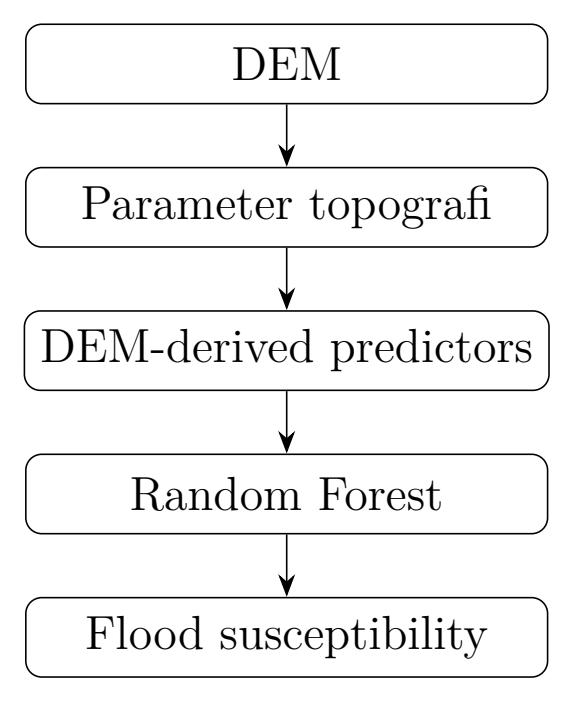
\includegraphics[width=0.34\textwidth,height=0.20\textheight,keepaspectratio]{figures/tikz_alur_topografi.png}
\vspace{4pt}
\end{center}

Untuk menguji sumber elevasi, setiap parameter turunan DEM dihitung dengan
prosedur yang sama untuk setiap produk, sedangkan prediktor non-DEM
dipertahankan tetap.

Daftar final prediktor telah ditetapkan dan dirinci lengkap pada
Subbab~3.6, terdiri atas 5 prediktor yang dihitung dari produk elevasi yang
diuji (elevasi, \textit{slope}, tiga representasi \textit{aspect}), 11
prediktor lingkungan non-DEM (hidrologi, hujan antecedent, indeks spektral),
serta 8 variabel \textit{dummy} tutupan lahan WorldCover (total 24
prediktor). Susunan dan fitur tersebut mengikuti praktik pada penelitian
acuan sekaligus ketersediaan data di Google Earth Engine
\citep{hakim2026}, sehingga setiap prediktor memiliki dasar rujukan.

\subsection{Random Forest untuk Flood Susceptibility}

Random Forest merupakan metode \textit{ensemble learning} yang membangun
sejumlah \textit{decision tree} dan menggabungkan hasil prediksinya
\citep{breiman2001}. Metode ini banyak digunakan dalam pemodelan spasial
karena mampu menangani hubungan nonlinier dan interaksi antarvariabel.

Dalam penelitian sebelumnya \citep{hakim2026}, Random Forest menghasilkan
kinerja tertinggi di antara tujuh model yang dibandingkan berdasarkan
ROC-AUC (\textit{Area Under the Receiver Operating Characteristic} curve),
meskipun perbedaan dengan beberapa model teratas tidak signifikan secara
statistik.

Oleh karena itu, penelitian ini menggunakan Random Forest sebagai
model yang dikontrol. Fokusnya bukan membandingkan Random Forest dengan model lain, melainkan
mempertahankannya sebagai algoritma pemodelan agar pengujian berpusat pada
sumber elevasi.

Secara mekanistik, setiap \textit{decision tree} dibangun pada sampel
bootstrap dari data latih (bagging), dan pada setiap titik pemisahan
simpul hanya sebagian kecil variabel yang dipertimbangkan (\textit{random
subspace}) \citep{breiman2001}. Kedua sumber kerandoman tersebut membuat
pohon-pohon yang dibangun relatif kurang berkorelasi satu sama lain, sehingga
pengagregasian rata-rata antarpohon mampu menurunkan varians prediksi.
Keluaran model berupa probabilitas banjir yang dihitung dari proporsi
suara kelas antarpohon, dan probabilitas tersebut yang kemudian dipetakan
sebagai \textit{susceptibility}.

\subsection{Sensitivitas Sumber Elevasi dalam Pemodelan Banjir}

Studi Meadows dkk.\ menunjukkan bahwa produk DEM global memiliki
karakteristik galat yang berbeda dan bahwa pengaruh tersebut dapat berkaitan
dengan tutupan lahan, slope, dan kondisi medan \citep{meadows2024}. Tique
dkk.\ juga menunjukkan bahwa perubahan DEM dan metode hidrologi dapat
menghasilkan perbedaan pada \textit{flood susceptibility mapping} di Nigeria
\citep{Tique2026}. Pengaruh karakteristik dan resolusi DEM juga dilaporkan pada pemodelan banjir
berbasis hidrolika \citep{fatdillah2022,fikri2026}.

Namun, penelitian yang sekaligus mengubah beberapa komponen dapat
menyulitkan interpretasi mengenai faktor mana yang sebenarnya menyebabkan
perubahan hasil. Oleh karena itu, penelitian ini menggunakan desain
eksperimen terkontrol:

\begin{center}
Sumber elevasi berubah, sedangkan komponen lainnya dipertahankan.
\end{center}

Secara sederhana, tiga eksperimen yang dibangun adalah:

\begin{center}
\begin{tabular}{ccc}
Eksperimen A: SRTM & Eksperimen B: GLO-30 & Eksperimen C: AW3D30 \\
$\downarrow$ & $\downarrow$ & $\downarrow$ \\
RF & RF & RF \\
$\downarrow$ & $\downarrow$ & $\downarrow$ \\
susceptibility & susceptibility & susceptibility \\
\end{tabular}
\end{center}

Ketiga keluaran dibandingkan untuk mengukur
\textit{DEM-source sensitivity}.

Pengukuran sensitivitas tersebut menuntut kehati-hatian evaluasi. Titik
sampel yang saling berdekatan dalam ruang geografis cenderung memiliki
nilai prediktor dan label yang serupa (autokorelasi spasial), sehingga
pemisahan latih-uji yang dilakukan secara acak pada tingkat titik
cenderung memberi estimasi performa yang terlalu optimis
\citep{roberts2017,ploton2020}. Oleh karena itu, uji ketahanan hasil pada
penelitian ini menempatkan penilaian spasial sebanding dengan penilaian
performa: metrik performa dilengkapi validasi silang spasial berbasis blok,
sedangkan selisih performa antar-DEM dievaluasi melalui resampling pada
tingkat blok dilengkapi interval kepercayaan (Subbab~3.8).

\subsection{Tutupan Lahan sebagai Stratifikasi}

Kesalahan dan karakteristik produk elevasi dapat berbeda menurut kondisi
permukaan. Meadows dkk.\ menunjukkan bahwa \textit{land cover} merupakan
faktor penting yang menjelaskan variasi galat elevasi, terutama pada area
berhutan \citep{meadows2024}.

Oleh karena itu, ESA WorldCover digunakan bukan sebagai perlakuan utama,
tetapi sebagai variabel stratifikasi \citep{zanaga2021}. Tujuannya
adalah menjawab pertanyaan berikut:

\begin{quote}
Apakah sensitivitas hasil \textit{susceptibility} terhadap pergantian DEM
sama pada seluruh tutupan lahan?
\end{quote}

Dengan demikian, analisis tidak berhenti pada perbandingan tiga peta secara
keseluruhan.

\subsection{Penelitian Terdahulu}

Tabel~\ref{tab:prior} merangkum penelitian yang paling relevan beserta
posisi penelitian ini terhadap masing-masing studi.

\begin{table}[!htbp]
\centering
\caption[Penelitian terdahulu yang relevan]{Penelitian terdahulu yang relevan.}
\label{tab:prior}
\begin{adjustbox}{max width=\textwidth}
\begin{tabular}{>{\raggedright}p{2.6cm}
                >{\raggedright}p{3.6cm}
                >{\raggedright}p{3.8cm}
                >{\raggedright\arraybackslash}p{3.8cm}}
\toprule
\textbf{Penelitian} & \textbf{Fokus} & \textbf{Yang Diadopsi} & \textbf{Modifikasi pada penelitian ini} \\
\midrule
Fatdillah dkk.\ (2022) \citep{fatdillah2022} & Pengaruh DEM terhadap \textit{flood modelling} & Gagasan bahwa input elevasi dapat memengaruhi hasil banjir & Diuji dalam kerangka \textit{machine learning} terkontrol \\
Meadows dkk.\ (2024) \citep{meadows2024} & Perbandingan global produk DEM & Dasar bahwa produk elevasi mempunyai karakteristik/galat berbeda & Dampak DEM ditelusuri sampai output \textit{susceptibility} \\
Yuwono dkk.\ (2024) \citep{yuwono2024} & Perbandingan DEM pada pemodelan hidrolika banjir Semarang & Konteks perbandingan DEM di wilayah studi & Diuji pada kerangka \textit{machine learning} \\
Verdyansyah dkk.\ (2025) \citep{verdyansyah2025} & \textit{Machine learning} + banjir di Kabupaten Demak & Konteks pemodelan banjir berbasis \textit{machine learning} lokal & Sumber elevasi divariasikan secara sistematis \\
Hakim dkk.\ (SMDS) \citep{hakim2026} & Sentinel-1 + tujuh model untuk \textit{flood susceptibility} Semarang--Demak & \textit{Flood inventory} Sentinel-1 dan baseline Random Forest & RF dipertahankan dan DEM dijadikan faktor eksperimen \\
Fikri dkk.\ (2026) \citep{fikri2026} & Pengaruh karakteristik/resolusi DEM terhadap \textit{flood modelling} & Sensitivitas output terhadap data elevasi & Fokus pada \textit{source sensitivity} dan \textit{spatial susceptibility} \\
Studi Tique dkk.\ (2026) \citep{Tique2026} & Multi-DEM + ML \textit{flood susceptibility} & Bukti empiris bahwa pilihan DEM berpengaruh & Fokus variasi sumber DEM pada satu algoritme RF \\
\bottomrule
\end{tabular}
\end{adjustbox}
\end{table}

Studi Tique dkk.\ \citep{Tique2026} secara eksplisit membandingkan empat DEM,
beberapa metode hidrologi, dan tiga model \textit{machine learning} pada
pemetaan \textit{flood susceptibility}. Hasilnya menunjukkan bahwa variasi
pilihan DEM maupun metode hidrologi memengaruhi hasil pemetaan.

Perbedaan rancangan tersebut memperlihatkan posisi penelitian ini secara
faktual: penelitian
Tique dkk.\ mengombinasikan perubahan DEM, metode hidrologi, dan
model ML dalam satu rancangan pembandingan, sedangkan penelitian ini
memutar satu faktor saja --- sumber elevasi --- dengan komponen lain
dipertahankan tetap, sehingga keterkaitan perubahan keluaran dengan
pergantian sumber elevasi terbaca secara langsung. Orientasi perlakuan
tunggal pada satu faktor menjadi ciri rancangan penelitian ini.

\subsection{Kerangka Teori}

Kerangka teori penelitian diringkas dalam rangkaian alur berikut:

\begin{figure}[H]
\centering
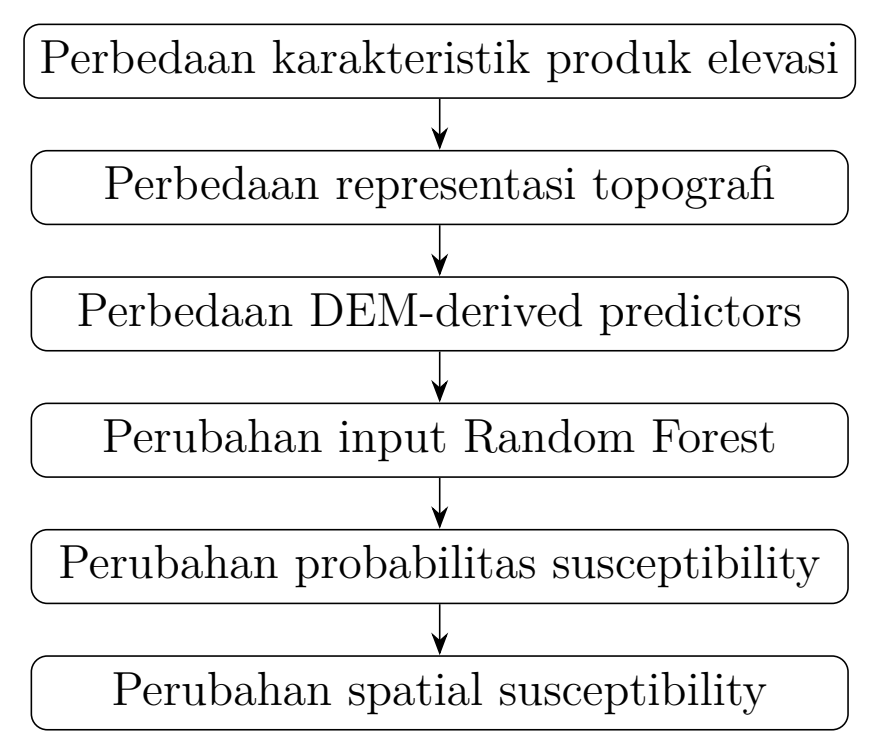
\includegraphics[width=0.46\textwidth,height=0.18\textheight,keepaspectratio]{figures/tikz_kerangka_teori.png}
\caption[Kerangka teori penelitian]{Kerangka teori rangkaian alur dari sumber produk elevasi
sampai keluaran \textit{flood susceptibility}.}
\label{fig:kerangka-teori}
\end{figure}

Kerangka pada Gambar~\ref{fig:kerangka-teori} menjelaskan bahwa sumber
produk elevasi menjadi titik awal pada rangkaian alur tersebut. Selanjutnya,
kondisi permukaan digunakan untuk menjelaskan variasinya: perbedaan
spasial \textit{susceptibility} dipetakan terhadap kelas tutupan lahan ESA
WorldCover, sehingga sensitivitas sumber elevasi dapat dibandingkan antar
tutupan lahan.

\subsection{Kerangka Berpikir}

Alur penelitian pada Gambar~\ref{fig:kerangka} menunjukkan bahwa
\textit{flood inventory} Sentinel-1 dan prediktor non-elevasi berada di luar
perlakuan, dengan sumber produk elevasi untuk lima prediktor turunan DEM
sebagai faktor perlakuan, sementara prediktor lainnya dipertahankan sama.
Ketiga peta \textit{susceptibility} yang dihasilkan kemudian
dibandingkan pada tingkat performa dan spasial, sebelum dianalisis lebih
lanjut menurut kelas tutupan lahan.

\begin{figure}[H]
\centering
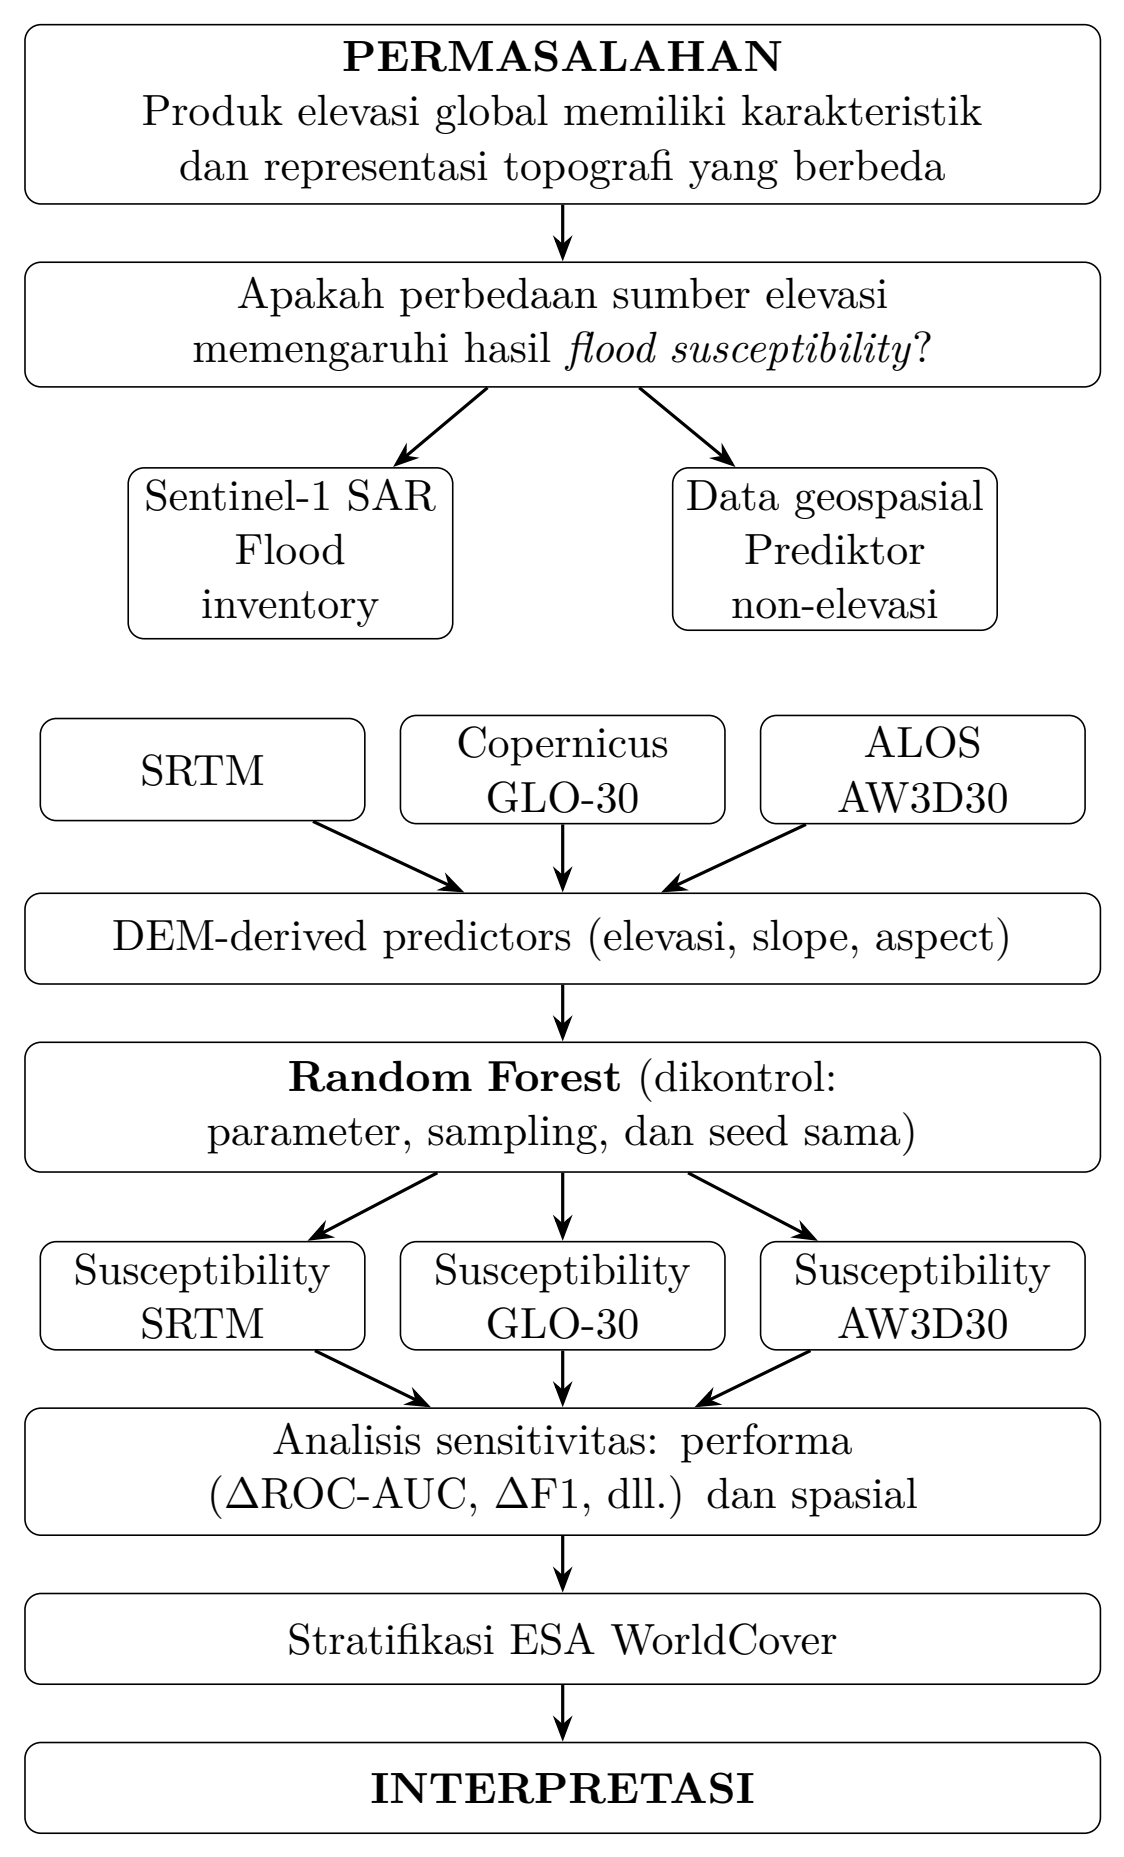
\includegraphics[width=0.58\textwidth,height=0.31\textheight,keepaspectratio]{figures/tikz_kerangka_berpikir.png}
\caption{Kerangka berpikir penelitian.}
\label{fig:kerangka}
\end{figure}

%==================================================================
% BAB III
%==================================================================

\clearpage
\bab{Metode Penelitian}

\subsection{Pendekatan dan Desain Penelitian}

Penelitian kuantitatif ini menggunakan desain
eksperimen terkontrol untuk menguji sensitivitas hasil
\textit{flood susceptibility mapping} terhadap pemilihan produk elevasi.
Faktor perlakuan, yaitu sumber produk elevasi, memiliki tiga level:

\begin{enumerate}
\item SRTM;
\item Copernicus DEM GLO-30;
\item ALOS AW3D30.
\end{enumerate}

Pada ketiga eksperimen, model Random Forest, \textit{flood inventory},
wilayah penelitian, prediktor non-elevasi, preprocessing, sampling, dan
evaluasi dipertahankan sama. Dengan demikian, perbandingan berfokus pada
sumber elevasi (Tabel~\ref{tab:desain}).

\begin{table}[!htbp]
\centering
\caption[Desain eksperimen penelitian]{Desain eksperimen penelitian.}
\label{tab:desain}
\begin{tabular}{ll}
\toprule
\textbf{Komponen} & \textbf{Kondisi} \\
\midrule
Faktor perlakuan & Produk elevasi \\
Level 1 & SRTM \\
Level 2 & Copernicus DEM GLO-30 \\
Level 3 & ALOS AW3D30 \\
Model ML & Random Forest \\
Flood inventory & Sama \\
Wilayah & Sama \\
Prediktor non-elevasi & Sama \\
Prosedur preprocessing & Sama \\
Prosedur sampling & Sama \\
Prosedur evaluasi & Sama \\
Analisis tambahan & Stratifikasi WorldCover \\
\bottomrule
\end{tabular}
\end{table}

\subsection{Wilayah Penelitian}

Wilayah penelitian berada pada kawasan pesisir Semarang--Demak, Jawa Tengah,
Indonesia. Wilayah tersebut dipilih karena memiliki karakteristik dataran
rendah, kawasan pesisir, kawasan pertanian dan terbangun, serta riwayat
kejadian banjir yang membuat sensitivitas representasi topografi menjadi
relevan untuk dikaji \citep{marfai2008,Husnayaen2018,Sakina2025}.

Batas wilayah penelitian mengikuti area pesisir Kota Semarang dan Kabupaten
Demak (administrasi provinsi Jawa Tengah tingkat 2, FAO GAUL) yang sama
dengan yang digunakan pada penelitian SMDS sebelumnya agar konteks
wilayah dan sumber data dapat dibandingkan secara konsisten
\citep{hakim2026}.

\subsection{Data dan Sumber Data}

Sumber data penelitian merupakan gabungan produk penginderaan jauh dan data
turunan yang tersedia pada katalog Google Earth Engine, meliputi citra
Sentinel-1 untuk \textit{flood inventory}, tiga produk elevasi sebagai
perlakuan, serta data pendukung untuk prediktor dan stratifikasi. Sumber,
bentuk keluaran, resolusi, produsen, dan fungsi masing-masing data dalam
penelitian dirangkum pada Tabel~\ref{tab:data}.

\begin{table}[!htbp]
\centering
\caption[Matriks data penelitian]{Matriks data penelitian: sifat sumber, bentuk keluaran, unit
pengukuran, produsen, katalog Google Earth Engine, dan fungsi dalam
penelitian.}
\label{tab:data}
\small
\begin{adjustbox}{max width=\textwidth}
\begin{tabular}{>{\raggedright}p{2.5cm}>{\raggedright}p{2.5cm}>{\raggedright}p{1.55cm}>{\raggedright}p{1.4cm}>{\raggedright}p{3.55cm}>{\raggedright\arraybackslash}p{2.2cm}}
\toprule
\textbf{Data} & \textbf{Jenis/sifat} & \textbf{Bentuk \& resolusi} & \textbf{Unit} & \textbf{Produsen; ID katalog GEE} & \textbf{Fungsi (RM)} \\
\midrule
Sentinel-1 GRD (\textit{Ground Range Detected}) & Radar SAR pita-C; pra \& pasca kejadian & Citra GRD/IW 10 m & dB & ESA Copernicus; \texttt{COPERNICUS/\allowbreak S1\_GRD} & Pembentukan \textit{flood inventory} (RM 2, RM 4) \\
SRTM & Radar C-band interferometri; DSM & Grid 30 m & m & NASA/USGS; \texttt{USGS/\allowbreak SRTMGL1\_003} & Perlakuan elevasi 1 (RM 1, RM 2) \\
Copernicus DEM GLO-30 & Radar bistatik pita-X TanDEM-X; DSM & Grid 30 m & m & ESA Copernicus (GMES); \texttt{COPERNICUS/\allowbreak DEM/\allowbreak GLO30} & Perlakuan elevasi 2 (RM 1, RM 2) \\
ALOS AW3D30 (V4.1) & Stereo fotogrametri optik PRISM; DSM & Grid 30 m & m & JAXA; \texttt{JAXA/\allowbreak ALOS/\allowbreak AW3D30/\allowbreak V4\_1} & Perlakuan elevasi 3 (RM 1, RM 2) \\
MERIT Hydro & Turunan DEM aplikasi hidrologi & Grid 90 m & m / log & Univ. Tokyo (Yamazaki dkk.); \texttt{MERIT/\allowbreak Hydro/\allowbreak v1\_0\_1} & HAND, aliran hulu, lebar \& jarak sungai (RM 2) \\
JRC Global Surface Water & Rekap air permukaan 1984--2021 & Citra raster; pita \textit{occ} & \% & Komisi Eropa (JRC); \texttt{JRC/\allowbreak GSW1\_4/\allowbreak GlobalSurfaceWater} & Masking air permanen; jarak air (RM 2, RM 4) \\
CHIRPS harian & Klimatologi hujan IR + stasiun & Grid $0{,}05^{\circ}$ (5,5 km) & mm/hari & UCSB CHG; \texttt{UCSB-CHG/\allowbreak CHIRPS/\allowbreak DAILY} & Hujan antecedent 7 \& 30 hari (RM 2) \\
Sentinel-2 SR (L2A) & Citra permukaan optik multispektral & Citra 10--60 m & refl.\ (SR) & ESA Copernicus; \texttt{COPERNICUS/\allowbreak S2\_SR\_HARMONIZED} & NDVI, NDWI, MNDWI, NDBI (RM 2) \\
ESA WorldCover (v200) & Klasifikasi tutupan lahan 11 kelas & Citra 10 m & kode kelas & ESA; \texttt{ESA/\allowbreak WorldCover/\allowbreak v200} & Variabel \textit{dummy} + stratifikasi (RM 2, RM 3, RM 4) \\
\bottomrule
\end{tabular}
\end{adjustbox}
\end{table}

\subsection{Perangkat Penelitian}

Penelitian utama dilakukan menggunakan Google Earth Engine untuk akuisisi
dan preprocessing data spasial \citep{gorelick2017}. Pengolahan data dan
pemodelan Random Forest dapat dilakukan menggunakan lingkungan
Python/Google Colab apabila diperlukan.

Penggunaan Google Earth Engine dipilih karena menyediakan akses terhadap
berbagai dataset penginderaan jauh dan geospasial pada lingkungan komputasi
yang sama, sehingga ketiga produk elevasi dapat diolah dengan prosedur yang
konsisten.

\subsection{Pembentukan Flood Inventory}
\label{ssec:flood-inventory}

Flood inventory dibentuk menggunakan citra Sentinel-1 SAR. Tahapan utamanya:

\begin{enumerate}
\item penyusunan komposit Sentinel-1 pra-kejadian dan pasca-kejadian;
\item preprocessing citra SAR;
\item perhitungan perubahan \textit{backscatter} antarperiode;
\item identifikasi area yang mengalami perubahan konsisten dengan genangan;
\item masking perairan permanen menggunakan JRC Global Surface Water
\citep{pekel2016};
\item pembentukan label \textit{flood}/\textit{non-flood}.
\end{enumerate}

Pendekatan ini mengikuti prinsip pembentukan label banjir berbasis perubahan
Sentinel-1 yang digunakan dalam penelitian SMDS sebelumnya \citep{hakim2026}
serta praktik \textit{change detection} yang terdokumentasi
\citep{islammeng2022,unspider2024}. Seluruh parameter ambang dan periode
kejadian ditetapkan mengikuti konfigurasi penelitian acuan \citep{hakim2026}
dan diterapkan identik pada ketiga eksperimen:

\begin{itemize}
\item komposit median polarisasi VH untuk periode pra-kejadian
(25 Februari--12 Maret 2024) dan pasca-kejadian (15--31 Maret 2024);
\item kriteria piksel banjir: rasio daya \textit{backscatter} pra-kejadian
terhadap pasca-kejadian $>1{,}25$ dan daya VH pasca-kejadian $<-18$~dB;
\item piksel berada di luar perairan permanen JRC Global Surface Water
(\textit{occurrence} $\geq 80\%$);
\item kemiringan lereng SRTM $<5^{\circ}$ untuk menyaring artefak geometrik
radar \citep{hakim2026};
\item penyaringan konektivitas spasial minimum 8 piksel.
\end{itemize}

Label dibentuk satu kali dari citra dan parameter yang sama, kemudian
digunakan identik pada ketiga eksperimen, sehingga perbedaan hasil
antarperlakuan berasal dari sumber elevasi dan bukan dari perbedaan label.

Kriteria kemiringan lereng di bawah $5^{\circ}$ digunakan untuk mengurangi
kemungkinan masuknya piksel dengan karakteristik lereng yang berpotensi
menghasilkan artefak pada inventori banjir, misalnya artefak geometris
radar pita-C (\textit{layover} dan \textit{foreshortening}) pada area
berlereng curam, bukan membatasi domain pesisir.
Karena acuan lereng berasal dari SRTM, label ini tidak sepenuhnya independen
terhadap karakteristik satu produk perlakuan. Implikasi hal tersebut
dipertimbangkan dalam pembahasan pada Subbab~4.8. Peta \textit{flood inventory}
hasil deteksi perubahan Sentinel-1 beserta sebaran titik sampel induk dan
pembagian 16 blok validasi silang spasial disajikan pada Gambar~\ref{fig:study-area}.

\begin{figure}[!htbp]
\centering
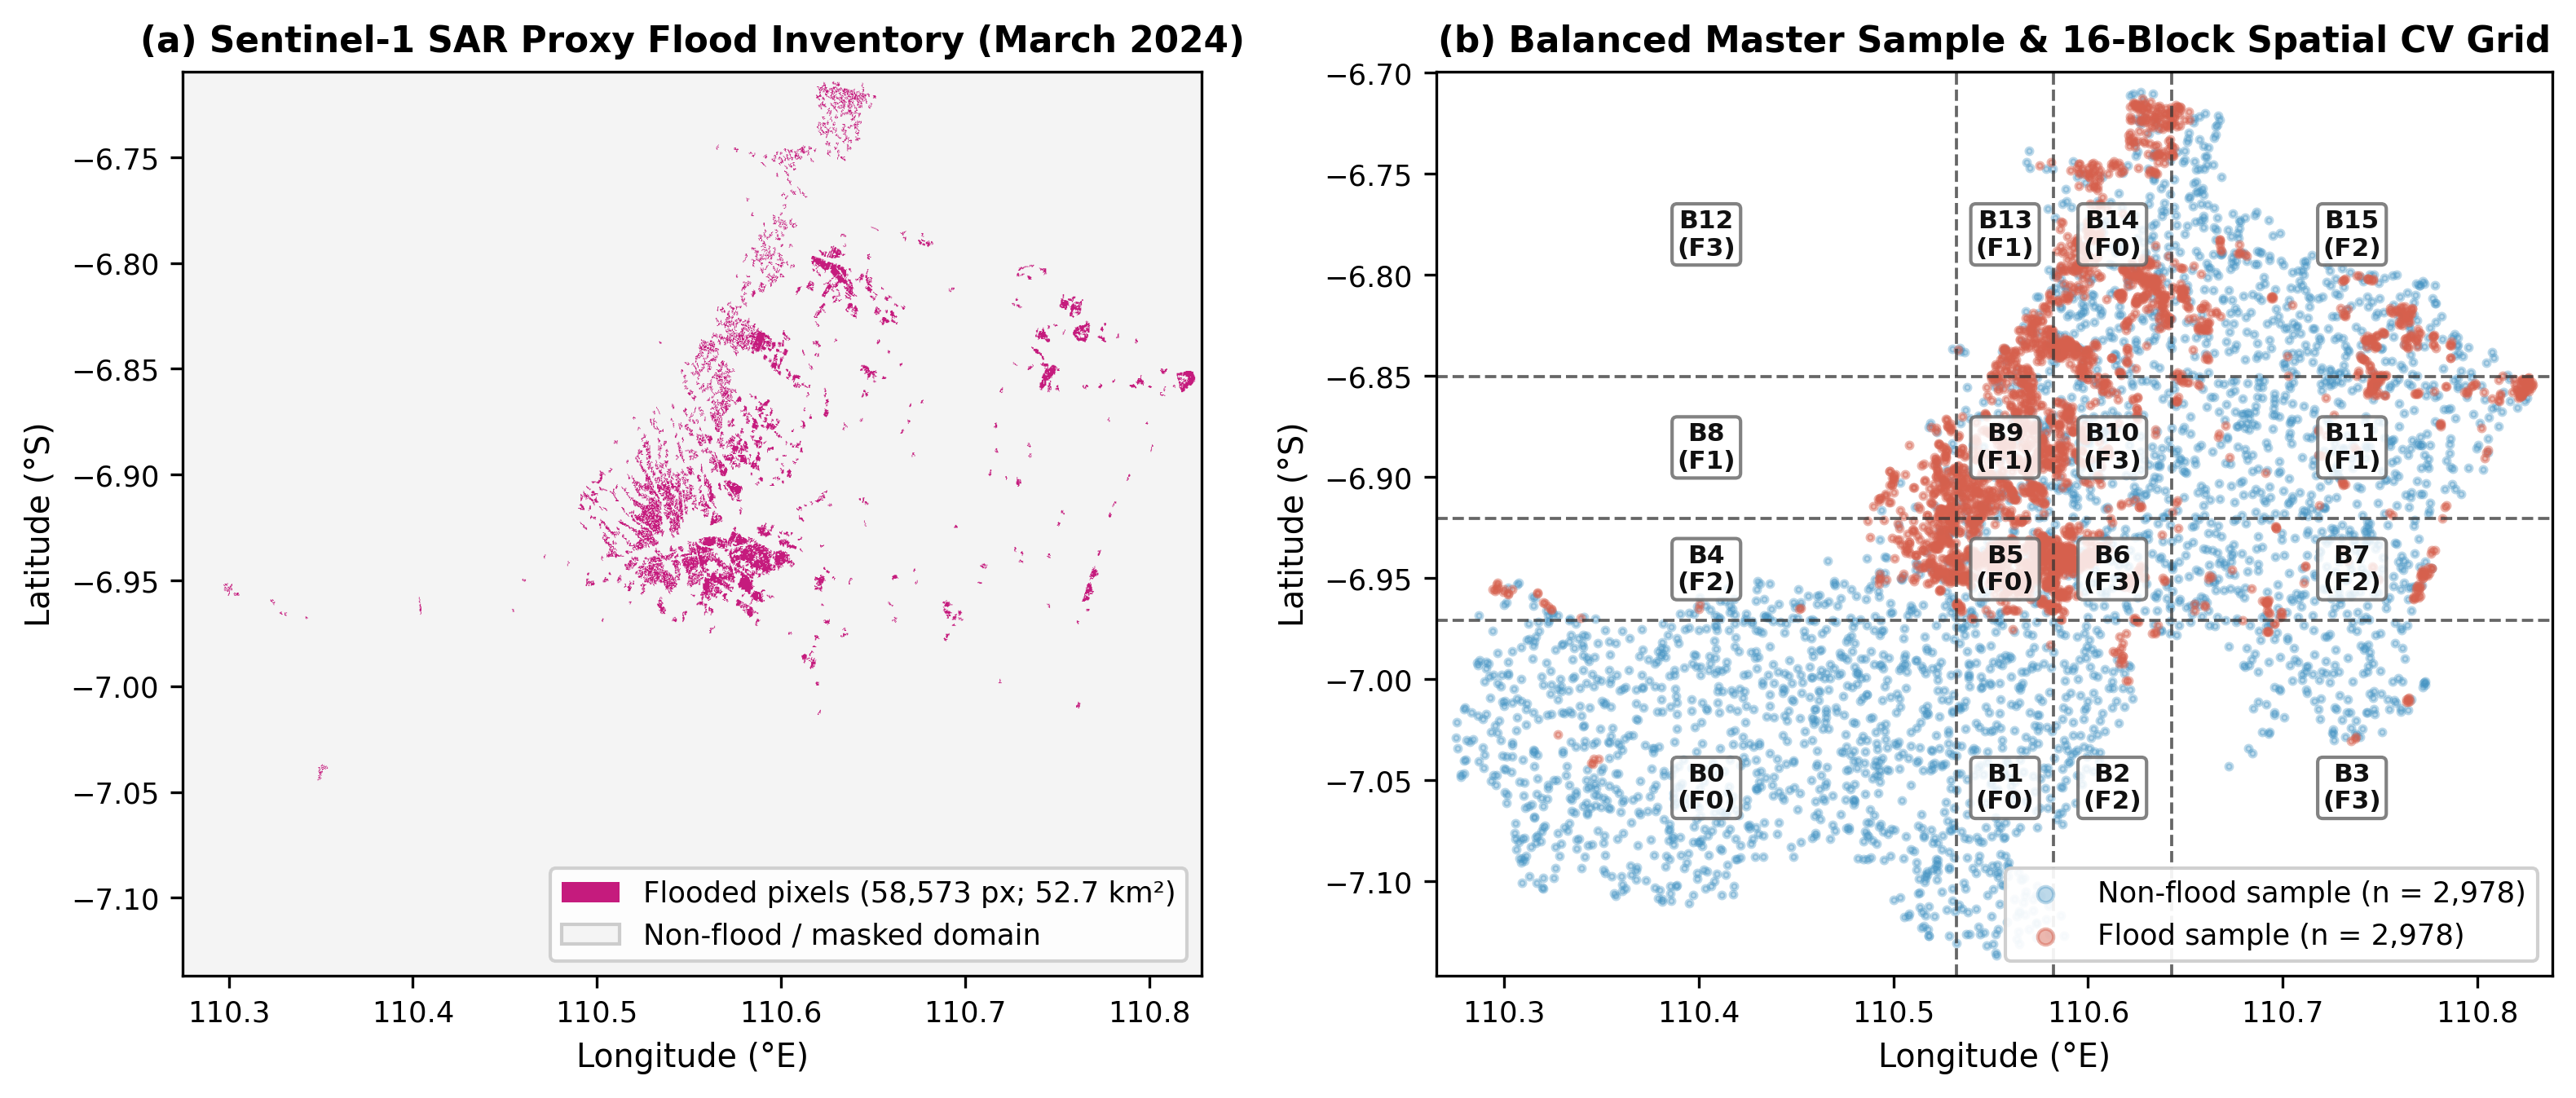
\includegraphics[width=0.92\textwidth,height=0.38\textheight,keepaspectratio]{figures/fig_study_area_samples.png}
\caption[Wilayah kajian dan struktur pengambilan sampel]{Wilayah kajian dan struktur pengambilan sampel: (a) \textit{flood inventory} proksi Sentinel-1 SAR kejadian Maret 2024 di Semarang--Demak ($58.573$ piksel banjir); (b) sebaran spasial sampel induk berimbang ($n = 5.956$) beserta pembagian 16 blok kuantil koordinat (\texttt{B0}--\texttt{B15}) dan penugasan 4-\textit{fold} validasi silang spasial (\texttt{F0}--\texttt{F3}).}
\label{fig:study-area}
\end{figure}

\subsection{Pembentukan Prediktor}

Prediktor penelitian dibagi menjadi dua kelompok.

\subsubsection{DEM-derived predictors}

Prediktor yang diperoleh dari setiap produk elevasi terdiri atas lima fitur
dengan prosedur ekstraksi yang identik dihitung menggunakan modul terrain
Google Earth Engine (\texttt{ee.Terrain}):

\begin{itemize}
\item \textit{elevation} (elevasi permukaan, meter);
\item \textit{slope} (kemiringan lereng, derajat);
\item \textit{aspect}\textsubscript{sin} (komponen sinus arah lereng);
\item \textit{aspect}\textsubscript{cos} (komponen kosinus arah lereng);
\item \textit{aspect}\textsubscript{valid} (indikator validitas arah lereng).
\end{itemize}

Arah lereng (\textit{aspect}) pada dasarnya dinyatakan dalam sudut $0^{\circ}$
sampai $360^{\circ}$ sehingga mengandung diskontinuitas melingkar pada batas
$0^{\circ}$/$360^{\circ}$. Untuk menghindari kesalahan interpretasi nilai
sudut oleh model, \textit{aspect} direpresentasikan melalui dekomposisi
sinus dan kosinusnya, serta satu indikator biner yang menandai piksel dengan
arah lereng terdefinisi. Pada daerah datar, arah lereng tidak terdefinisi
sehingga kasus tersebut dipisahkan secara eksplisit oleh indikator. Kelima fitur tersebut
diulang identik untuk masing-masing produk elevasi yang diuji, sehingga jumlah
prediktor yang diturunkan dari DEM sama pada ketiga konfigurasi.

Ketiga produk DEM diproses menggunakan prosedur yang sama, termasuk
penyelarasan grid, clipping wilayah penelitian, serta dokumentasi perbedaan
acuan vertikal (EGM96 pada SRTM, EGM2008 pada Copernicus
DEM GLO-30, dan EGM96 pada ALOS AW3D30; ketiganya menyatakan tinggi
ortometrik terhadap model geoid \textit{Earth Gravitational Model})
yang kritis pada dataran pesisir rendah.

\subsubsection{Prediktor non-elevasi dan dummy tutupan lahan}

Prediktor yang tidak dihitung dari produk elevasi perlakuan dipertahankan
sama pada ketiga eksperimen dan mengikuti set pada penelitian acuan
\citep{hakim2026}. Sebelas prediktor non-elevasi terdiri atas:

\begin{itemize}
\item variabel hidrologi dari MERIT Hydro \citep{yamazaki2019}: HEIGHT
Above Nearest Drainage (HAND), logaritma luas aliran hulu
(\textit{upstream drainage area}), lebar sungai (\textit{river width}), dan
jarak ke sungai terdekat;
\item jarak ke badan air permanen JRC Global Surface Water
\citep{pekel2016};
\item curah hujan antecedent CHIRPS \citep{funk2015} berupa akumulasi 7 hari
dan 30 hari sebelum kejadian;
\item indeks spektral Sentinel-2 \citep{saha2021}: NDVI
(\textit{Normalized Difference Vegetation Index}), NDWI
(\textit{Normalized Difference Water Index}), MNDWI (\textit{Modified
Normalized Difference Water Index}), dan NDBI (\textit{Normalized
Difference Built-up Index}).
\end{itemize}

Prediktor hidrologi MERIT Hydro memuat informasi topografi yang
diturunkan dari \textit{MERIT DEM}, bukan dari produk elevasi perlakuan.
Karena bersumber dari satu produk dan dipertahankan identik pada semua
perlakuan, prediktor ini bukan sumber variasi antarperlakuan. Namun,
kandungan topografinya tetap perlu diperhitungkan saat prediktor ini
ditafsirkan sebagai variabel non-elevasi.

Delapan variabel \textit{dummy} tutupan lahan dihasilkan dari
kategorisasi kelas ESA WorldCover \citep{zanaga2021} (kode 10 tutupan pohon,
30 padang rumput, 40 lahan pertanian, 50 kawasan terbangun, 60 lahan tanpa
vegetasi, 80 badan air, 90 lahan basah herba, dan 95 mangrove). Kelas
tutupan semak belukar (kode 20) tidak muncul pada sampel utama sehingga tidak
menghasilkan variabel dummy pada evaluasi tersebut. Dengan demikian, jumlah
total prediktor pada evaluasi utama menjadi
$5+11+8=24$ variabel prediktor.

\subsection{Eksperimen Random Forest Terkontrol}

Eksperimen dilakukan sebanyak tiga perlakuan:

\begin{description}
\item[Eksperimen 1] SRTM $\rightarrow$ DEM-derived predictors $\rightarrow$
prediktor non-elevasi yang sama $\rightarrow$ Random Forest $\rightarrow$
\textit{Susceptibility Map} SRTM.
\item[Eksperimen 2] Copernicus GLO-30 $\rightarrow$ DEM-derived predictors
$\rightarrow$ prediktor non-elevasi yang sama $\rightarrow$ Random Forest
$\rightarrow$ \textit{Susceptibility Map} GLO-30.
\item[Eksperimen 3] ALOS AW3D30 $\rightarrow$ DEM-derived predictors
$\rightarrow$ prediktor non-elevasi yang sama $\rightarrow$ Random Forest
$\rightarrow$ \textit{Susceptibility Map} AW3D30.
\end{description}

Ketiga eksperimen menggunakan \textit{flood inventory} yang sama sehingga
label tidak menjadi sumber variasi antarperlakuan. Demikian pula \textit{seed}
sampling, pembagian data latih-uji, dan parameter Random Forest dipertahankan
identik antarperlakuan.

Konfigurasi Random Forest yang digunakan adalah sebagai berikut. Peta
probabilitas spasial dibangun di Google Earth Engine menggunakan
\texttt{ee.Classifier.smileRandomForest} dengan 300 pohon, sedangkan
evaluasi metrik dilakukan pada implementasi Random Forest scikit-learn
dengan 400 pohon, jumlah minimum sampel pada simpul daun
(\textit{minimum samples leaf}) 2,
pemberatan kelas \textit{balanced} (\texttt{class\_weight}), dan
\textit{random state} yang disamakan antarperlakuan. Kedua implementasi
tidak dipandang sebagai satu model yang sama. Jalur GEE memakai kode tutupan
lahan sebagai satu masukan dan melatih model pada seluruh
sampel beku utama, sedangkan jalur scikit-learn memakai variabel dummy
tutupan lahan dan pemisahan sampel untuk evaluasi. Representasi 17 masukan GEE berbeda dari 24 masukan pada evaluasi utama
scikit-learn. Metrik scikit-learn bukan validasi langsung terhadap
model pembentuk peta GEE. Perbandingan antarproduk elevasi dipertahankan
dalam masing-masing jalur, bukan sebagai bukti kesetaraan kedua implementasi.
Pengambilan sampel dilakukan secara seimbang dengan menargetkan 3.000 sampel
untuk masing-masing kelas (\textit{seed}~42). Setelah proses ekstraksi
prediktor, sampel yang memiliki nilai prediktor tidak lengkap dieliminasi
melalui penyaringan \texttt{notNull}. Selanjutnya, dilakukan penyeimbangan
jumlah sampel antarkelas sehingga diperoleh 2.978 sampel banjir dan 2.978
sampel nonbanjir untuk pemodelan. Data kemudian dibagi 75\% latih dan 25\%
uji dan diperlakukan identik pada
ketiga perlakuan. Estimasi ketahanan hasil terhadap efek autokorelasi
spasial dan pilihan \textit{seed} dilaporkan melalui pengecekan dengan
validasi silang spasial dan \textit{block bootstrap} pada Subbab~3.8.

\subsection{Evaluasi Model}

Evaluasi dilakukan dengan membandingkan metrik ketiga eksperimen pada data
pengujian yang sama secara metodologis. Ukuran evaluasi meliputi ROC-AUC
(\textit{Area Under the Receiver Operating Characteristic} curve),
accuracy, precision, recall, dan F1-score. ROC-AUC mengukur kemampuan
diskriminasi keseluruhan tanpa bergantung pada ambang, sedangkan accuracy,
precision, recall, dan F1-score dihitung pada ambang klasifikasi tetap
$0{,}5$. Ukuran-ukuran tersebut mengikuti praktik evaluasi klasifikasi biner
pada penelitian \textit{flood susceptibility} berbasis \textit{machine
learning} \citep{hakim2026}.

Sebagai pelaporan tambahan, ambang klasifikasi alternatif dihitung menggunakan
indeks Youden \citep{youden1950} pada kurva ROC, yaitu
$J(t)=\text{Sens}(t)+\text{Spec}(t)-1$ dengan ambang $t$ yang memaksimalkan
$J$. Indeks ini hanya diperlakukan sebagai informasi pelaporan dan tidak
dipakai sebagai metrik utama karena ambangnya ditentukan pada data uji yang
sama dengan metrik yang sedang dinilai, sehingga rentan memberikan hasil yang
cenderung optimistis.

Karena titik sampel yang berdekatan cenderung memiliki nilai prediktor dan
label yang serupa (autokorelasi spasial), pembagian latih-uji acak pada
tingkat titik berpotensi menghasilkan estimasi performa yang terlalu optimis
\citep{roberts2017,ploton2020}. Evaluasi performa karena itu diperkuat dengan
tiga skema pengecekan yang identik pada ketiga perlakuan:

\begin{itemize}
\item validasi silang spasial 4-\textit{fold}: ruang kajian dibagi
menjadi 16 blok berdasarkan kuantil lintang dan bujur; empat blok dipilih
bergiliran sebagai blok uji; model dilatih ulang pada blok pelatihan dan
dievaluasi pada blok uji yang dipisahkan spasial; hasil dilaporkan sebagai
rata-rata metrik lintas \textit{fold} yang dihitung dari probabilitas
prediksi pada piksel uji;
\item block bootstrap: selisih ROC-AUC antarproduk diresampling
1.000 kali dengan pengembalian pada 16 blok yang sama; setiap pasangan
produk dievaluasi pada sampel ulang blok yang identik sehingga kesalahan
sampling dihitung berpasangan; interval kepercayaan 95\% diambil dari
distribusi selisih pada sampel ulang blok. Sebaran sampel ulang ini mengukur
ketidakpastian selisih atas rangkaian 16 blok yang sama dan bukan berarti
1.000 unit data independen;
\item pengujian multi-\textit{seed}: lima nilai \textit{seed}
(42, 100, 2024, 7, dan 99) diulang dari tahap sampling hingga evaluasi,
termasuk ekstraksi fitur dan pembagian data, untuk memeriksa konsistensi
arah peringkat antarproduk.
\end{itemize}

\subsubsection{Diagnostik Autokorelasi Spasial}

Data kejadian banjir bersifat spasial, sehingga nilai pada lokasi yang
berdekatan cenderung lebih mirip daripada nilai pada lokasi yang berjauhan.
Gejala ini disebut autokorelasi spasial. Pada penelitian ini sumbernya jelas,
sebab elevasi, kemiringan lereng, jarak ke sungai, dan genangan berubah
secara kontinu di ruang. Akibatnya amatan tidak saling bebas, dan pembagian
data latih dan uji secara acak membuat titik uji hampir selalu memiliki
tetangga dekat di data latih.

Kondisi tersebut melahirkan \textit{spatial leakage}, yaitu bocornya
informasi lingkungan lokasi uji ke dalam proses pelatihan. Model dapat tampak
akurat karena mengenali lingkungan sekitar titik uji, bukan karena
mempelajari hubungan antara prediktor dan banjir yang dapat digeneralisasi ke
wilayah baru. Karena itu penelitian ini memakai \textit{spatial
cross-validation} dengan 16 blok kuantil koordinat yang dibagi ke dalam empat
\textit{fold}. Pada setiap \textit{fold}, model dilatih ulang tanpa blok uji,
sehingga probabilitas out-of-fold (OOF) pada tiap titik berasal dari model
yang tidak pernah melihat blok titik tersebut. Fungsi \textit{spatial
cross-validation} adalah mengurangi \textit{leakage} melalui rancangan
pembagian data. Rancangan ini belum sempurna karena blok yang bersebelahan
tidak dipisahkan zona penyangga, sehingga titik di tepi blok tetap dapat
berdekatan dengan data latih.

Global Moran's I \citep{moran1950} dipakai untuk menggambarkan seberapa kuat
suatu variabel mengelompok secara spasial. Untuk nilai $x_i$ pada $n$ lokasi,
bobot spasial $w_{ij}$ yang distandardisasi per baris sehingga
$S_0=\sum_{i}\sum_{j}w_{ij}=n$, dan $z_i=x_i-\bar{x}$, statistiknya adalah
\[
I=\frac{n}{S_0}\,\frac{\sum_{i}\sum_{j}w_{ij}\,z_i\,z_j}{\sum_{i}z_i^{2}},
\qquad E[I]=-\frac{1}{n-1}.
\]
Nilai $I$ di atas $E[I]$ menunjukkan pengelompokan nilai yang mirip, nilai di
bawah $E[I]$ menunjukkan pola berselang-seling.

Pengujian dirumuskan sebagai berikut.
\begin{itemize}
\item $H_0$: nilai tersebar acak secara spasial (tidak ada autokorelasi
      spasial).
\item $H_1$: terdapat autokorelasi spasial (uji dua sisi).
\item Taraf signifikansi $\alpha=0{,}05$.
\item Kriteria penolakan: tolak $H_0$ jika $p$-value lebih kecil dari
      $\alpha$.
\item $p$-value dihitung dengan permutasi kondisional. Nilai $x_i$ diacak
      lintas lokasi yang tetap sebanyak $B=9.999$ kali (\textit{seed}~42),
      lalu
      \[
      p=\frac{1+\#\{|I_{\mathrm{perm}}-E[I]|\ge
      |I_{\mathrm{obs}}-E[I]|\}}{B+1}.
      \]
      Dengan $B=9.999$, $p$ terkecil yang dapat dilaporkan adalah
      $1/(B+1)=0{,}0001$. Untuk peta raster dipakai $B=999$ karena jumlah
      pikselnya sangat besar.
\end{itemize}

Dua kelompok data dianalisis.
\begin{enumerate}
\item \textit{Probabilitas OOF dan residual OOF pada titik sampel.}
      Probabilitas $\hat{p}_i^{OOF}$ berasal dari \textit{spatial
      cross-validation} evaluasi utama, dan residual dihitung sebagai
      $r_i=y_i-\hat{p}_i^{OOF}$ dengan $y_i$ label aktual. Prediksi data
      latih tidak dipakai karena sudah dilihat model dan akan membuat
      residual tampak lebih kecil dan lebih acak dari yang sebenarnya.
\item \textit{Peta probabilitas kerawanan per DEM} (raster hasil Random
      Forest GEE 300 pohon). Peta dilatih pada seluruh sampel, sehingga
      analisis ini menggambarkan struktur spasial permukaan prediksi dan
      bukan kinerja \textit{out-of-fold}.
\end{enumerate}

Unit analisis adalah titik sampel, bukan 16 blok. Agregasi ke 16 unit tidak
layak karena blok kuantil sangat tidak seimbang (satu blok hanya memuat 1
titik, median 305 titik, maksimum 967 titik, dan ada blok tanpa salah satu
kelas). Selain itu, 16 unit memberi daya uji yang sangat rendah, menimbulkan
masalah \textit{modifiable areal unit} (hasil bergantung pada cara batas
blok ditarik), dan menghapus struktur di dalam blok, padahal blok adalah
satuan pembagian \textit{fold}.

Bobot spasial untuk titik adalah $k$ tetangga terdekat ($k=8$) dengan jarak
dihitung dalam meter pada UTM zona~49S dan distandardisasi per baris. Pilihan
ini sesuai karena titik sampel tersebar tidak beraturan dengan kepadatan yang
sangat bervariasi (jarak tetangga terdekat bermedian sekitar 149 m dan
mencapai 1,5 km), sehingga ambang jarak tetap akan menyisakan titik tanpa
tetangga di area jarang dan terlalu banyak tetangga di area padat. Metode
KNN menjamin setiap titik memiliki jumlah tetangga yang sama. Uji kepekaan
memakai $k=5$ dan $k=12$. Definisi bobot dibangun sekali dari koordinat dan
dipakai identik untuk ketiga DEM, dengan deret permutasi yang sama, sehingga
perbandingan antar-DEM adil. Untuk raster dipakai \textit{queen contiguity}
(8 tetangga) yang distandardisasi per baris pada grid yang sama untuk ketiga
DEM.

Moran's I adalah analisis diagnostik pendukung. Statistik ini menggambarkan
struktur spasial probabilitas dan galat, tetapi tidak menghilangkan
\textit{spatial leakage} dan tidak membuktikan ketiadaannya. Pencegahan
\textit{leakage} tetap bergantung pada rancangan evaluasi spasial. Hasil yang
tidak signifikan tidak dibaca sebagai bukti tidak adanya autokorelasi, karena
dapat disebabkan oleh daya uji, pilihan bobot spasial, atau asumsi
keterpertukaran pada uji permutasi. Perbedaan nilai $I$ antar-DEM tidak diuji
secara inferensial pada tahap ini.

\subsection{Analisis Sensitivitas}

Analisis sensitivitas membandingkan keluaran ketiga eksperimen pada dua
tingkat.

\subsubsection{Sensitivitas performa}

Tingkat pertama mengukur perubahan metrik kinerja model, yaitu perubahan
ROC-AUC, accuracy, precision, recall, dan F1-score antarperlakuan. Selisih
ROC-AUC antarproduk dilaporkan bersama interval kepercayaan hasil
\textit{block bootstrap} pada Subbab~3.8 agar perubahan dapat dinilai
terhadap ketidakpastian estimasi.

\subsubsection{Sensitivitas spasial}

Tingkat kedua mengukur perubahan keluaran spasial antarpeta probabilitas dan
peta kelas. Ukuran yang dilaporkan:

\begin{itemize}
\item rerata selisih probabilitas absolut, $\overline{|\Delta p|}$,
yaitu rerata nilai $|p_a - p_b|$ terhadap seluruh piksel wilayah kajian
untuk sepasang peta $a$ dan $b$;
\item kesesuaian kelas (\textit{spatial agreement}), yaitu
persentase piksel yang masuk ke kelas kerawanan yang sama pada kedua peta
setelah keduanya diklasifikasikan menjadi lima kelas dengan batas interval
yang sama;
\item luas setiap kelas kerawanan pada masing-masing peta;
\item matriks transisi antarkelas untuk setiap pasangan peta.
\end{itemize}

Perbandingan pada dua tingkat tersebut menjawab bukan hanya apakah keluaran
pemodelan berubah ketika sumber elevasi diganti, tetapi juga
di mana perubahan tersebut terkonsentrasi secara spasial.

\subsection{Stratifikasi Berdasarkan Tutupan Lahan}

ESA WorldCover digunakan untuk membagi wilayah penelitian berdasarkan kelas
tutupan lahan \citep{zanaga2021}. Kemudian perubahan \textit{susceptibility}
akibat pergantian DEM dihitung pada masing-masing kelompok, misalnya
kawasan terbangun, pertanian, dan vegetasi.

Analisis ini dilakukan untuk mengetahui apakah sensitivitas sumber elevasi
menunjukkan pola yang berbeda pada jenis permukaan tertentu. Dasarnya adalah
temuan Meadows dkk.\ bahwa \textit{land cover} merupakan salah satu faktor
utama yang berkaitan dengan variasi galat pada produk DEM global
\citep{meadows2024}.

\clearpage
\subsection{Tahapan Penelitian}

\begin{table}[H]
\small
\centering
\caption[Tahapan penelitian]{Tahapan penelitian.}
\label{tab:tahapan}
\begin{adjustbox}{max width=\textwidth}
\begin{tabular}{clp{5.4cm}p{4.6cm}}
\toprule
\textbf{Tahap} & \textbf{Kegiatan} & \textbf{Output} & \textbf{Orientasi RM} \\
\midrule
1 & Studi literatur & Dasar teori dan metode & Seluruh RM \\
2 & Penentuan AOI (\textit{area of interest}) & Wilayah penelitian & RM 1, RM 3, RM 4 \\
3 & Akuisisi Sentinel-1 & Data SAR & RM 2, RM 4 \\
4 & Pembentukan \textit{flood inventory} & Label \textit{flood/non-flood} & RM 2, RM 3, RM 4 \\
5 & Akuisisi tiga DEM & SRTM, GLO-30, AW3D30 & RM 1 \\
6 & Prapemrosesan DEM & DEM siap digunakan & RM 1 \\
7 & Ekstraksi prediktor turunan DEM & Prediktor topografi & RM 1 \\
8 & Penyusunan prediktor & Dataset pemodelan & RM 1, RM 2 \\
9 & Eksperimen Random Forest SRTM & Peta \textit{flood susceptibility} SRTM & RM 2 \\
10 & Eksperimen Random Forest GLO-30 & Peta \textit{flood susceptibility} GLO-30 & RM 2 \\
11 & Eksperimen Random Forest AW3D30 & Peta \textit{flood susceptibility} AW3D30 & RM 2 \\
12 & Evaluasi model & Metrik performa & RM 2, RM 3 \\
13 & Analisis sensitivitas spasial & Perubahan spasial peta & RM 3, RM 4 \\
14 & Stratifikasi WorldCover & Sensitivitas menurut tutupan lahan & RM 3, RM 4 \\
15 & Interpretasi & Kesimpulan sensitivitas DEM & Seluruh RM \\
\bottomrule
\end{tabular}
\end{adjustbox}
\end{table}

%==================================================================
% BAB IV
%==================================================================

\clearpage
\bab{Hasil dan Pembahasan}

Bab ini menyajikan hasil eksperimen terkontrol untuk satu kejadian banjir pada
satu wilayah kajian (\textit{Area of Interest}), dengan satu sampel induk
(\textit{master sample}) acak yang terdiri atas 2.978 titik banjir dan 2.978
titik non-banjir ($n=5.956$). Sampel induk dipertahankan identik pada ketiga
konfigurasi produk elevasi. Pada evaluasi utama scikit-learn, setiap model
Random Forest \citep{breiman2001} menggunakan 24 prediktor, yaitu 11 prediktor non-elevasi, 8 variabel
\textit{dummy} tutupan lahan, dan 5 prediktor topografi yang diturunkan dari
masing-masing produk DEM yang diuji. Pengolahan dilakukan menggunakan Google
Earth Engine dan lingkungan komputasi Kaggle (GPU T4). Statistik spasial pada
Subbab~4.5 dan~4.6 diturunkan dari eksperimen utama, dan ketahanan hasil
terhadap pembangkit acak diperiksa dengan lima nilai \textit{seed} yang
berbeda (Subbab~4.4).

Satu temuan metodologis perlu dicatat sejak awal. Pada uji awal, titik
non-banjir hanya terambil dari zona di sekitar perairan permanen JRC karena
pita \textit{occurrence} bersifat jarang (\textit{sparse}), sehingga piksel
daratan tanpa rekaman air ikut tersingkir saat \textit{masking}. Rata-rata
elevasi sampel non-banjir pada uji tersebut hanya $4{,}15$~m, jauh di bawah
rata-rata elevasi wilayah kajian sebesar $42{,}7$~m. Setelah \textit{masking}
diperbaiki dengan fungsi \texttt{unmask(0)}, populasi kandidat non-banjir
mencakup sekitar 97,9\% wilayah kajian. ROC-AUC validasi silang spasial pada
domain sempit di sekitar perairan hanya sekitar $0{,}70$, sedangkan pada
seluruh wilayah kajian mencapai $0{,}870$ hingga $0{,}890$. Selisih sekitar
$0{,}17$ ini menunjukkan bahwa hasil evaluasi perlu ditafsirkan dengan
mempertimbangkan desain pengambilan sampel kelas non-banjir, bukan sebagai
estimasi kausal pengaruh perluasan domain. Seluruh
hasil berikutnya berasal dari desain yang telah diperbaiki.

\subsection{Hasil Karakteristik Produk Elevasi}

Analisis statistik deskriptif pada grid resolusi 30~meter menunjukkan bahwa
ketiga produk elevasi global menghasilkan gambaran bentang lahan yang serupa
untuk wilayah kajian, yaitu dataran rendah pesisir pada bagian utara dan
perbukitan di bagian selatan. Perbedaan antarproduk menonjol pada elevasi
median di dataran rendah, yang tercermin pada statistik yang dilaporkan pada
paragraf ini.
Rata-rata elevasi pada wilayah penelitian tercatat sebesar $40{,}62$~m untuk
SRTM, $39{,}06$~m untuk Copernicus DEM GLO-30, dan $41{,}36$~m untuk ALOS
AW3D30, dengan nilai median masing-masing sebesar $8{,}50$~m, $4{,}94$~m, dan
$8{,}53$~m. Selisih (\textit{offset}) vertikal rata-rata terhadap SRTM adalah
$-1{,}56$~m pada Copernicus DEM GLO-30 dan $+0{,}39$~m pada ALOS AW3D30. Nilai
tersebut merupakan rerata selisih elevasi pada piksel yang valid pada
kedua produk yang dibandingkan, bukan pengurangan dua rerata wilayah
dengan cakupan valid yang dapat berbeda. Tidak dilakukan transformasi
koreksi vertikal. SRTM dan ALOS AW3D30 sama-sama memakai model geoid EGM96
sebagai acuan tinggi. Karena itu, selisih keduanya tidak dapat dijelaskan
oleh perbedaan model geoid. Copernicus DEM GLO-30 memakai EGM2008.
Selisih antarproduk dapat mencerminkan perbedaan karakteristik pengukuran
dan, pada pasangan yang berbeda model geoid, perbedaan acuan tinggi.
Kontribusi masing-masing belum dipisahkan dalam penelitian ini.
Sementara itu, rata-rata
kemiringan lereng (\textit{slope}) yang dihasilkan oleh masing-masing produk
adalah $3{,}03^{\circ}$ pada SRTM, $2{,}46^{\circ}$ pada Copernicus DEM GLO-30,
dan $3{,}13^{\circ}$ pada ALOS AW3D30. Statistik deskriptif lengkap untuk elevasi
dan kemiringan lereng pada seluruh grid wilayah kajian maupun pada titik sampel
banjir dan non-banjir disajikan pada Tabel~\ref{tab:dem-stats}.

\begin{table}[!htbp]
\small
\centering
\caption[Statistik deskriptif elevasi dan kemiringan lereng]{Statistik deskriptif elevasi (m) dan kemiringan lereng ($^\circ$) pada seluruh grid AOI Semarang--Demak ($N = 1.469.555$ piksel) serta pada titik sampel banjir ($n=2.978$) dan non-banjir ($n=2.978$).}
\label{tab:dem-stats}
\begin{adjustbox}{max width=\textwidth}
\begin{tabular}{ll rrrrrrr rr rr}
\toprule
& & \multicolumn{7}{c}{\textbf{Distribusi Grid Seluruh AOI ($N = 1.469.555$ piksel)}} & \multicolumn{2}{c}{\textbf{Sampel Banjir ($n=2.978$)}} & \multicolumn{2}{c}{\textbf{Non-Banjir ($n=2.978$)}} \\
\cmidrule(lr){3-9} \cmidrule(lr){10-11} \cmidrule(lr){12-13}
\textbf{Parameter} & \textbf{Produk DEM} & \textbf{Mean} & \textbf{SD} & $\boldsymbol{p_5}$ & $\boldsymbol{p_{25}}$ & $\boldsymbol{p_{50}}$ & $\boldsymbol{p_{75}}$ & $\boldsymbol{p_{95}}$ & \textbf{Mean} & \textbf{Median} & \textbf{Mean} & \textbf{Median} \\
\midrule
Elevasi (m) & SRTM & 40,62 & 76,09 & 0,60 & 4,53 & 8,50 & 24,60 & 234,51 & 3,25 & 3,00 & 42,67 & 8,00 \\
            & Copernicus GLO-30 & 39,06 & 75,72 & 1,18 & 2,96 & 4,94 & 22,97 & 233,00 & 1,99 & 1,40 & 41,12 & 6,30 \\
            & ALOS AW3D30 & 41,36 & 76,22 & 2,77 & 4,47 & 8,53 & 24,52 & 234,48 & 4,11 & 4,00 & 43,06 & 8,00 \\
\midrule
Slope ($^\circ$) & SRTM & 3,03 & 3,38 & 0,00 & 1,35 & 2,13 & 3,43 & 9,63 & 1,73 & 1,35 & 3,08 & 2,12 \\
                 & Copernicus GLO-30 & 2,46 & 3,99 & 0,14 & 0,36 & 0,87 & 2,87 & 10,62 & 0,39 & 0,28 & 2,59 & 0,93 \\
                 & ALOS AW3D30 & 3,13 & 4,02 & 0,00 & 0,95 & 1,90 & 3,43 & 10,92 & 1,32 & 0,96 & 3,17 & 1,91 \\
\bottomrule
\end{tabular}
\end{adjustbox}
\end{table}

\subsection{Hasil Flood Inventory}

Pembentukan \textit{flood inventory} diturunkan dari citra Sentinel-1 GRD
polarisasi VH (\textit{vertical transmit, horizontal receive}) menggunakan komposit median periode pra-kejadian
(25~Februari--12~Maret 2024) dan pasca-kejadian (15--31~Maret 2024).
Identifikasi genangan dilakukan menggunakan kriteria rasio daya
\textit{backscatter} sebelum terhadap sesudah kejadian sebesar lebih dari
$1{,}25$, nilai \textit{backscatter} pasca-kejadian kurang dari $-18$~dB,
berada di luar badan air permanen berdasarkan JRC Global Surface Water
(\textit{occurrence} $\geq 80\%$), memiliki kemiringan lereng kurang dari
$5^{\circ}$, serta memenuhi penyaringan konektivitas spasial minimum 8~piksel.
Prosedur dan parameter ini mengikuti rancangan pada penelitian acuan
\citep{hakim2026}, yang menghasilkan populasi piksel valid sebanyak 1.410.981
piksel non-banjir dan 58.573 piksel banjir. Label hasil ekstraksi ulang memiliki kecocokan 70\% terhadap 1.870 titik
sampel penelitian acuan \citep{hakim2026}. Selisih ini kemungkinan berkaitan
dengan pemrosesan ulang (\textit{reprocessing}) arsip Sentinel-1 di Google
Earth Engine. Kesetaraan dengan penelitian acuan karena itu terbatas pada
algoritma dan parameter, sedangkan perbandingan antarproduk pada
Subbab~4.4 tetap memakai himpunan label yang sama.

Evaluasi lebih lanjut terhadap karakteristik topografi pada 2.978 titik sampel
banjir menunjukkan bahwa lokasi genangan terkonsentrasi di kawasan dataran
rendah pesisir. Pada produk SRTM, median kemiringan lereng titik banjir
tercatat sebesar $1{,}35^{\circ}$ (persentil ke-99 sebesar $4{,}92^{\circ}$
dan maksimum $11{,}48^{\circ}$), sedangkan pada Copernicus DEM GLO-30 tercatat
sebesar $0{,}28^{\circ}$ (dengan 99,97\% titik berada di bawah $5^{\circ}$)
dan pada ALOS AW3D30 sebesar $0{,}96^{\circ}$ (dengan 98,76\% titik berada di
bawah $5^{\circ}$). Median elevasi pada titik-titik banjir tersebut
masing-masing adalah $3{,}0$~m untuk SRTM, $1{,}4$~m untuk Copernicus DEM
GLO-30, dan $4{,}0$~m untuk ALOS AW3D30. Selisih kemiringan lereng antarproduk
elevasi pada titik banjir tergolong kecil (median $|\Delta\text{slope}|$
berkisar antara $0{,}85^{\circ}$ hingga $1{,}24^{\circ}$) dan korelasi
antarproduk juga rendah (koefisien Spearman tidak melebihi $|0{,}07|$).
Sementara itu, sebagian besar titik banjir berada di bawah $5^{\circ}$ pada
ketiga produk (98,99\%, 99,97\%, dan 98,76\%). Pada sampel beku, 30 dari
2.978 titik banjir ($1{,}01\%$) memiliki prediktor \textit{slope} SRTM
sedikitnya $5^{\circ}$ (hingga $11{,}48^{\circ}$). Diagnostik empat rute di
Google Earth Engine pada ke-30 titik tersebut membuktikan bahwa saat
pembentukan label pada proyeksi asli \texttt{EPSG:4326} ($30{,}92$~m),
seluruh 30/30 titik ($100\%$) memiliki lereng di bawah $5^{\circ}$ (minimum
$1{,}32^{\circ}$, rerata $3{,}80^{\circ}$, maksimum $4{,}99^{\circ}$)
sehingga sah lolos filter \texttt{slope.lt(5)}. Sebaliknya, reproyeksi
bilinear SRTM ke grid \texttt{EPSG:32749} (30~m) sebelum perhitungan
\texttt{ee.Terrain.slope} pada ekstraksi prediktor menggeser jendela
$3\times3$ di tepi transisi piksel menjadi $5{,}10^{\circ}$--$11{,}48^{\circ}$
(selisih $0{,}000000^{\circ}$ terhadap tabel sampel induk). Karena acuan
penyaringan memakai SRTM, label juga tidak sepenuhnya independen terhadap
salah satu produk perlakuan, meskipun label diterapkan identik pada ketiga
eksperimen (Subbab~4.8). Perbandingan distribusi empiris elevasi dan kemiringan
lereng antara titik sampel banjir dan non-banjir pada ketiga produk elevasi
ditampilkan pada Gambar~\ref{fig:dem-characteristics}.

\begin{figure}[!htbp]
\centering
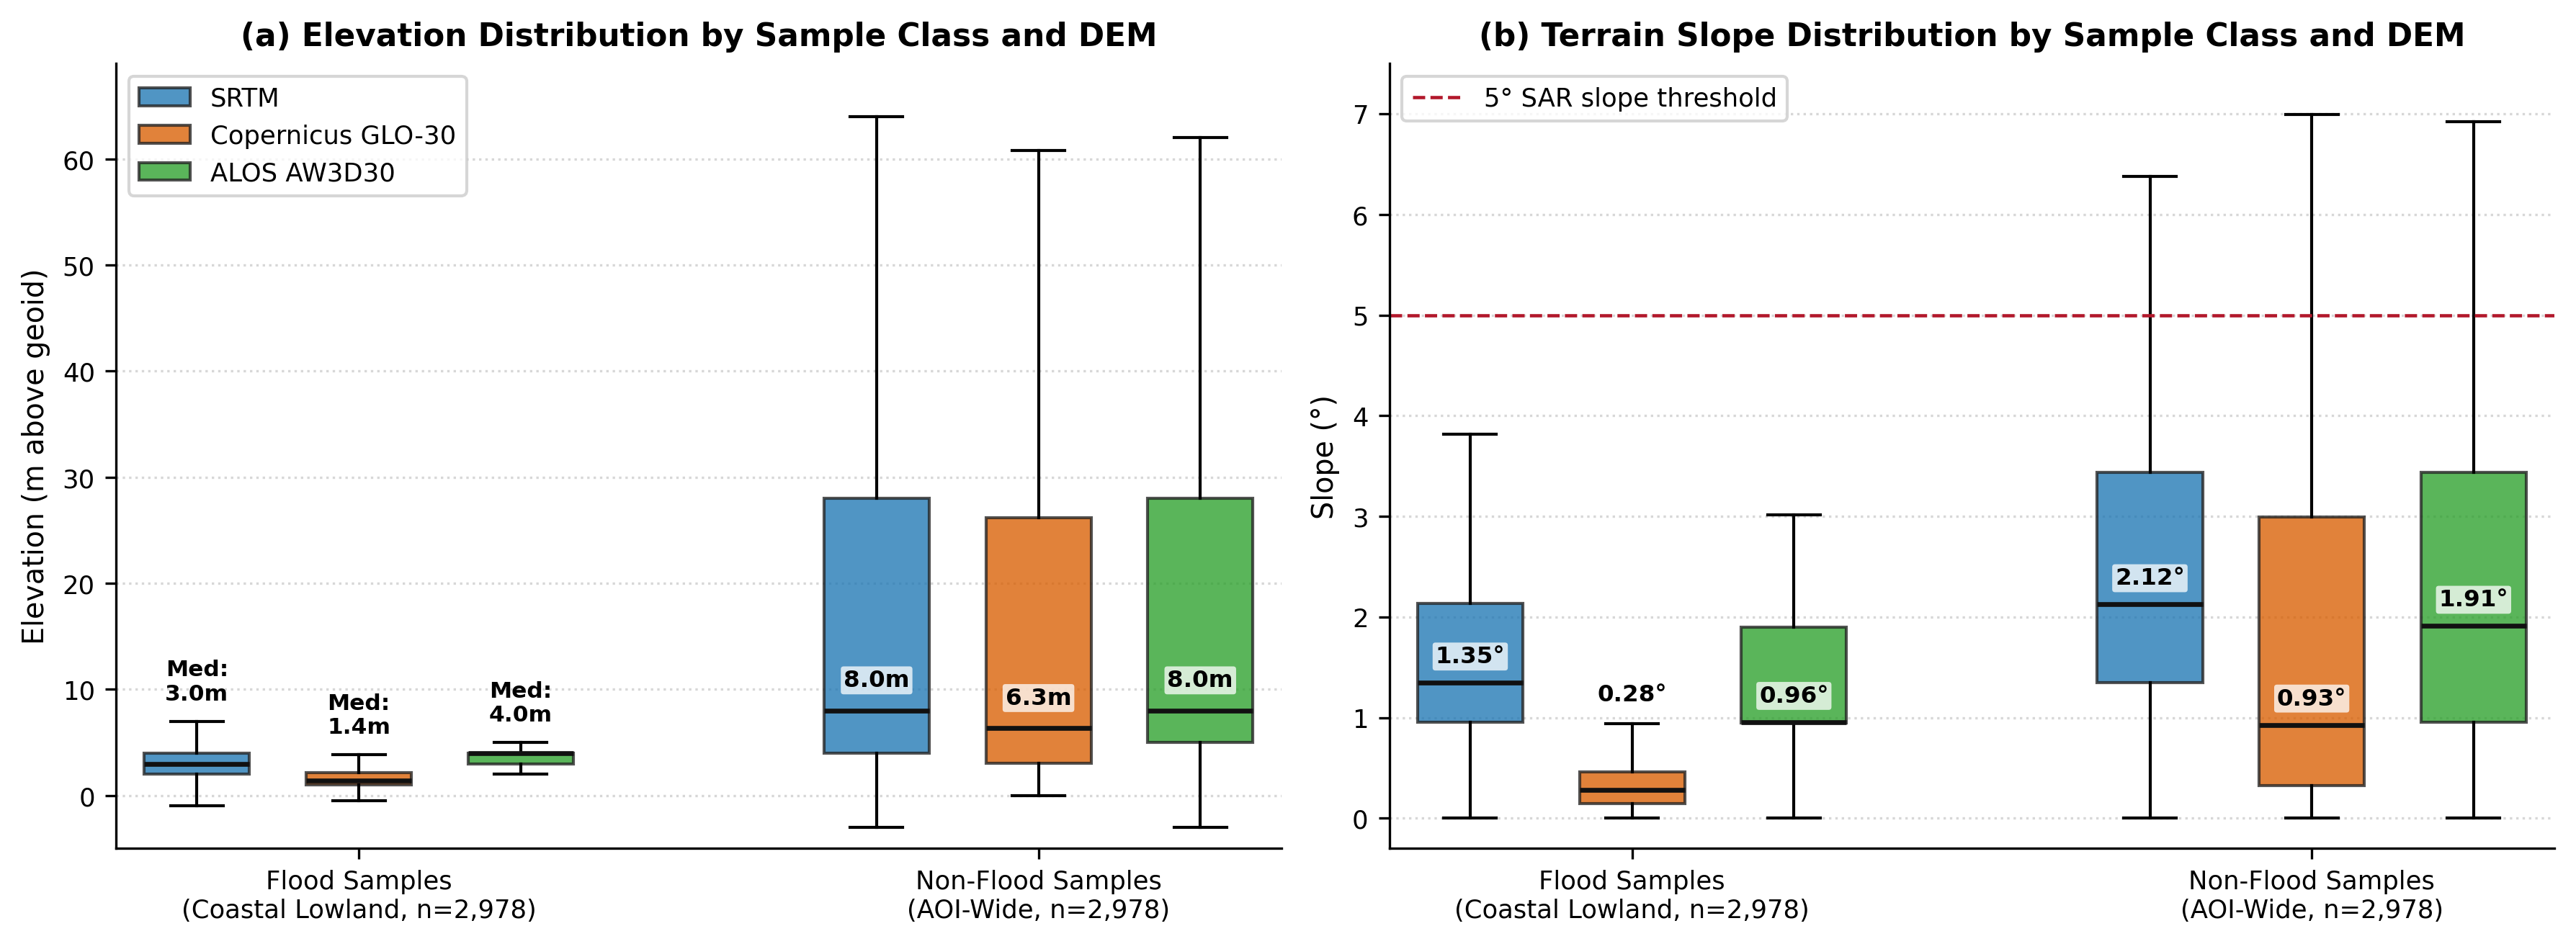
\includegraphics[width=0.92\textwidth,height=0.36\textheight,keepaspectratio]{figures/fig_dem_characteristics.png}
\caption[Distribusi empiris elevasi dan kemiringan lereng sampel]{Distribusi empiris (a) elevasi dan (b) kemiringan lereng pada titik sampel banjir ($n = 2.978$) dan non-banjir ($n = 2.978$) untuk SRTM, Copernicus DEM GLO-30, dan ALOS AW3D30.}
\label{fig:dem-characteristics}
\end{figure}

\subsection{Hasil Pemodelan Random Forest}

Pemodelan spasial untuk menghasilkan tiga peta probabilitas \textit{flood
susceptibility} dilakukan menggunakan algoritma \texttt{smileRandomForest}
pada Google Earth Engine dengan konfigurasi 300 pohon keputusan
(\textit{trees}) yang dilatih pada sampel induk yang sama. Probabilitas
prediksi yang dihasilkan selanjutnya dikelompokkan ke dalam lima kelas
kerawanan banjir (sangat rendah, rendah, sedang, tinggi, dan sangat tinggi)
menggunakan batas interval seragam sebesar $0{,}2$; $0{,}4$; $0{,}6$; dan
$0{,}8$ pada ketiga peta. Sementara itu, evaluasi kinerja prediktif pada skema
\textit{holdout} dilakukan menggunakan implementasi Random Forest pada pustaka
\textit{scikit-learn} (400~\textit{trees}) dengan pembagian data latih dan
data uji secara acak terstratifikasi sebesar 75:25 ($n_{\text{uji}}=1.489$).
Penentuan ambang klasifikasi optimal menggunakan indeks Youden \citep{youden1950} yang dihitung pada data uji hanya disajikan sebagai
informasi pelaporan tambahan karena sifatnya yang cenderung optimistis,
sedangkan metrik klasifikasi utama pada Tabel~\ref{tab:metrik-holdout}
dievaluasi pada ambang baku $0{,}5$. Seluruh statistik spasial peta, yang
meliputi distribusi luas kelas, matriks transisi antarkelas, dan stratifikasi
berdasarkan tutupan lahan, diturunkan dari keluaran model Google Earth Engine
(300~\textit{trees}) yang dilatih menggunakan sampel induk yang identik. Peta
probabilitas kerawanan banjir hasil ketiga konfigurasi ditampilkan pada
Gambar~\ref{fig:prob-maps}.

\begin{figure}[!htbp]
\centering
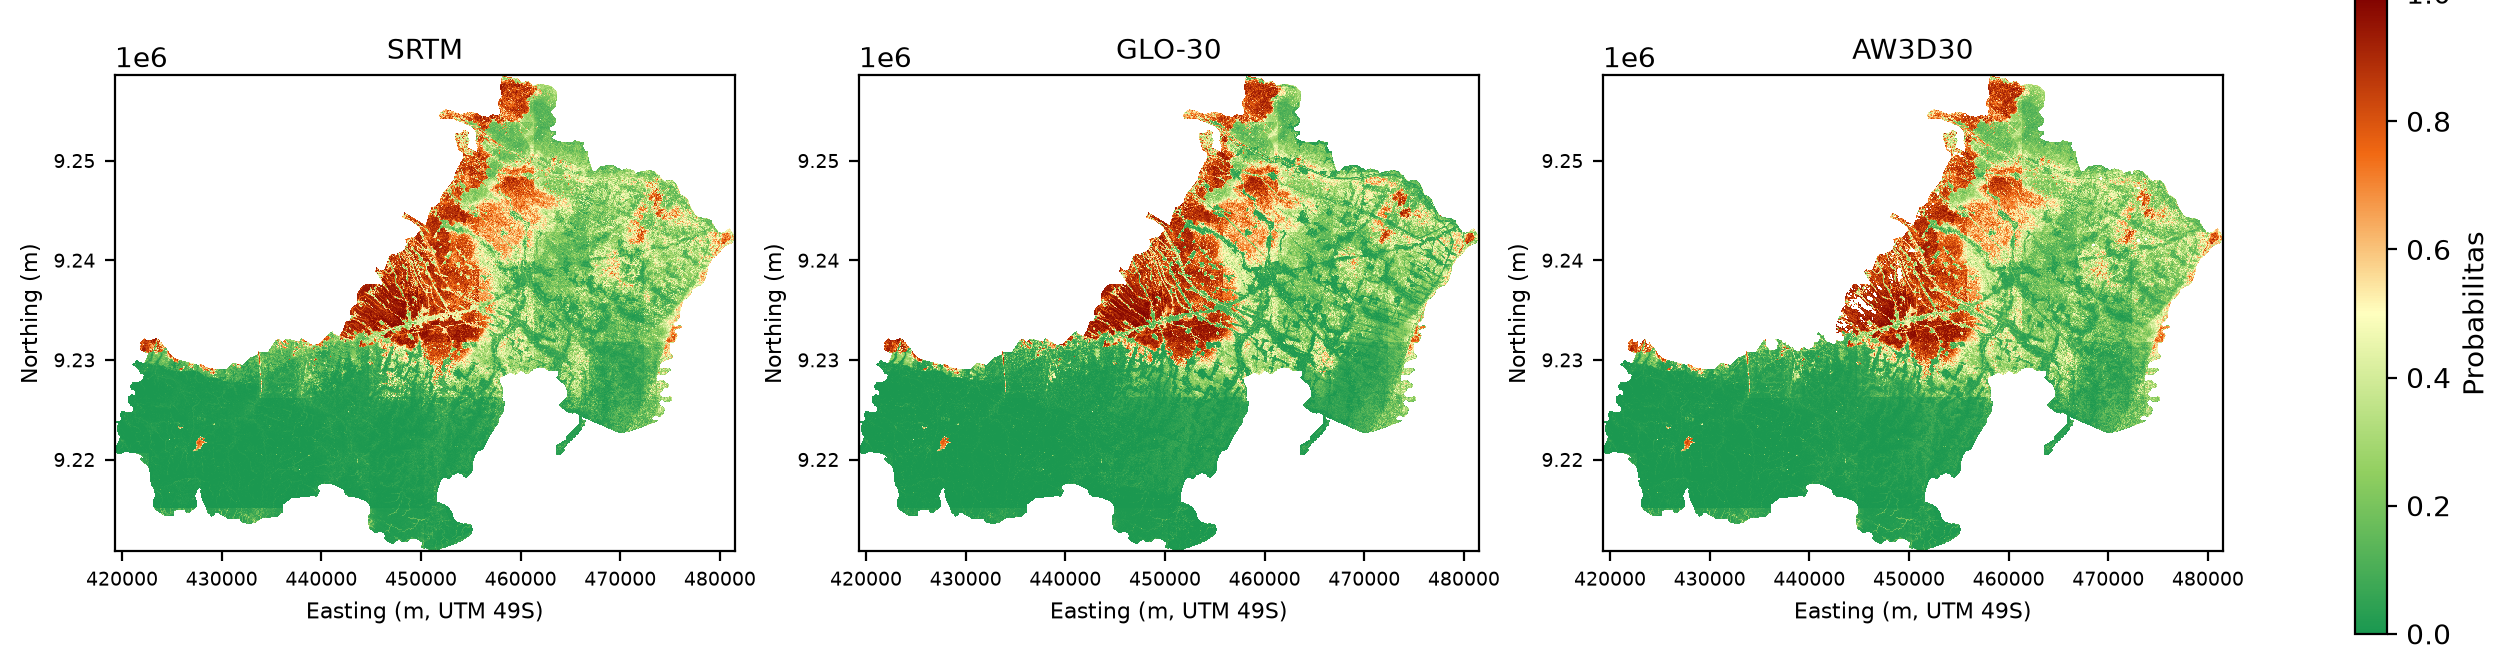
\includegraphics[width=0.95\textwidth,height=0.34\textheight,keepaspectratio]{figures/fig_prob_maps_id.png}
\caption[Peta probabilitas kerawanan banjir hasil Random Forest]{Peta probabilitas kerawanan banjir hasil Random Forest 300 pohon pada Google Earth Engine untuk ketiga konfigurasi produk elevasi, dengan batas kelas interval seragam $0{,}2$; $0{,}4$; $0{,}6$; dan $0{,}8$.}
\label{fig:prob-maps}
\end{figure}

\begin{table}[!htbp]
\small
\centering
\caption[Metrik evaluasi holdout pada masing-masing konfigurasi DEM]{Metrik evaluasi \textit{holdout} pada masing-masing konfigurasi DEM (pembagian acak terstratifikasi, $n_{\text{uji}}=1.489$; dilaporkan pada ambang baku $t = 0{,}50$ dan ambang optimal indeks Youden $t^*$).}
\label{tab:metrik-holdout}
\begin{adjustbox}{max width=\textwidth}
\begin{tabular}{l c cccc c cccc c}
\toprule
& & \multicolumn{4}{c}{\textbf{Ambang Klasifikasi Baku ($t = 0{,}50$)}} & & \multicolumn{4}{c}{\textbf{Ambang Optimal Indeks Youden ($t^*$)}} & \\
\cmidrule(lr){3-6} \cmidrule(lr){8-11}
\textbf{Konfigurasi DEM} & \textbf{ROC-AUC} & \textbf{Akurasi} & \textbf{Presisi} & \textbf{Recall} & \textbf{F1-Score} & $\boldsymbol{t^*}$ & \textbf{Akurasi} & \textbf{Presisi} & \textbf{Recall} & \textbf{F1-Score} & $\boldsymbol{\Delta}\textbf{AUC vs.\ SRTM}$ \\
\midrule
SRTM & 0,9318 & 0,8744 & 0,8468 & 0,9140 & 0,8791 & 0,5205 & 0,8791 & 0,8588 & 0,9073 & 0,8824 & $0{,}0000$ \\
Copernicus GLO-30 & \textbf{0,9404} & \textbf{0,8899} & \textbf{0,8580} & \textbf{0,9341} & \textbf{0,8945} & 0,4953 & \textbf{0,8912} & 0,8584 & \textbf{0,9368} & \textbf{0,8959} & $+0{,}0086$ \\
ALOS AW3D30 & 0,9360 & 0,8784 & 0,8488 & 0,9207 & 0,8833 & 0,5209 & 0,8805 & 0,8555 & 0,9153 & 0,8844 & $+0{,}0042$ \\
\bottomrule
\end{tabular}
\end{adjustbox}
\end{table}

\begin{figure}[!htbp]
\centering
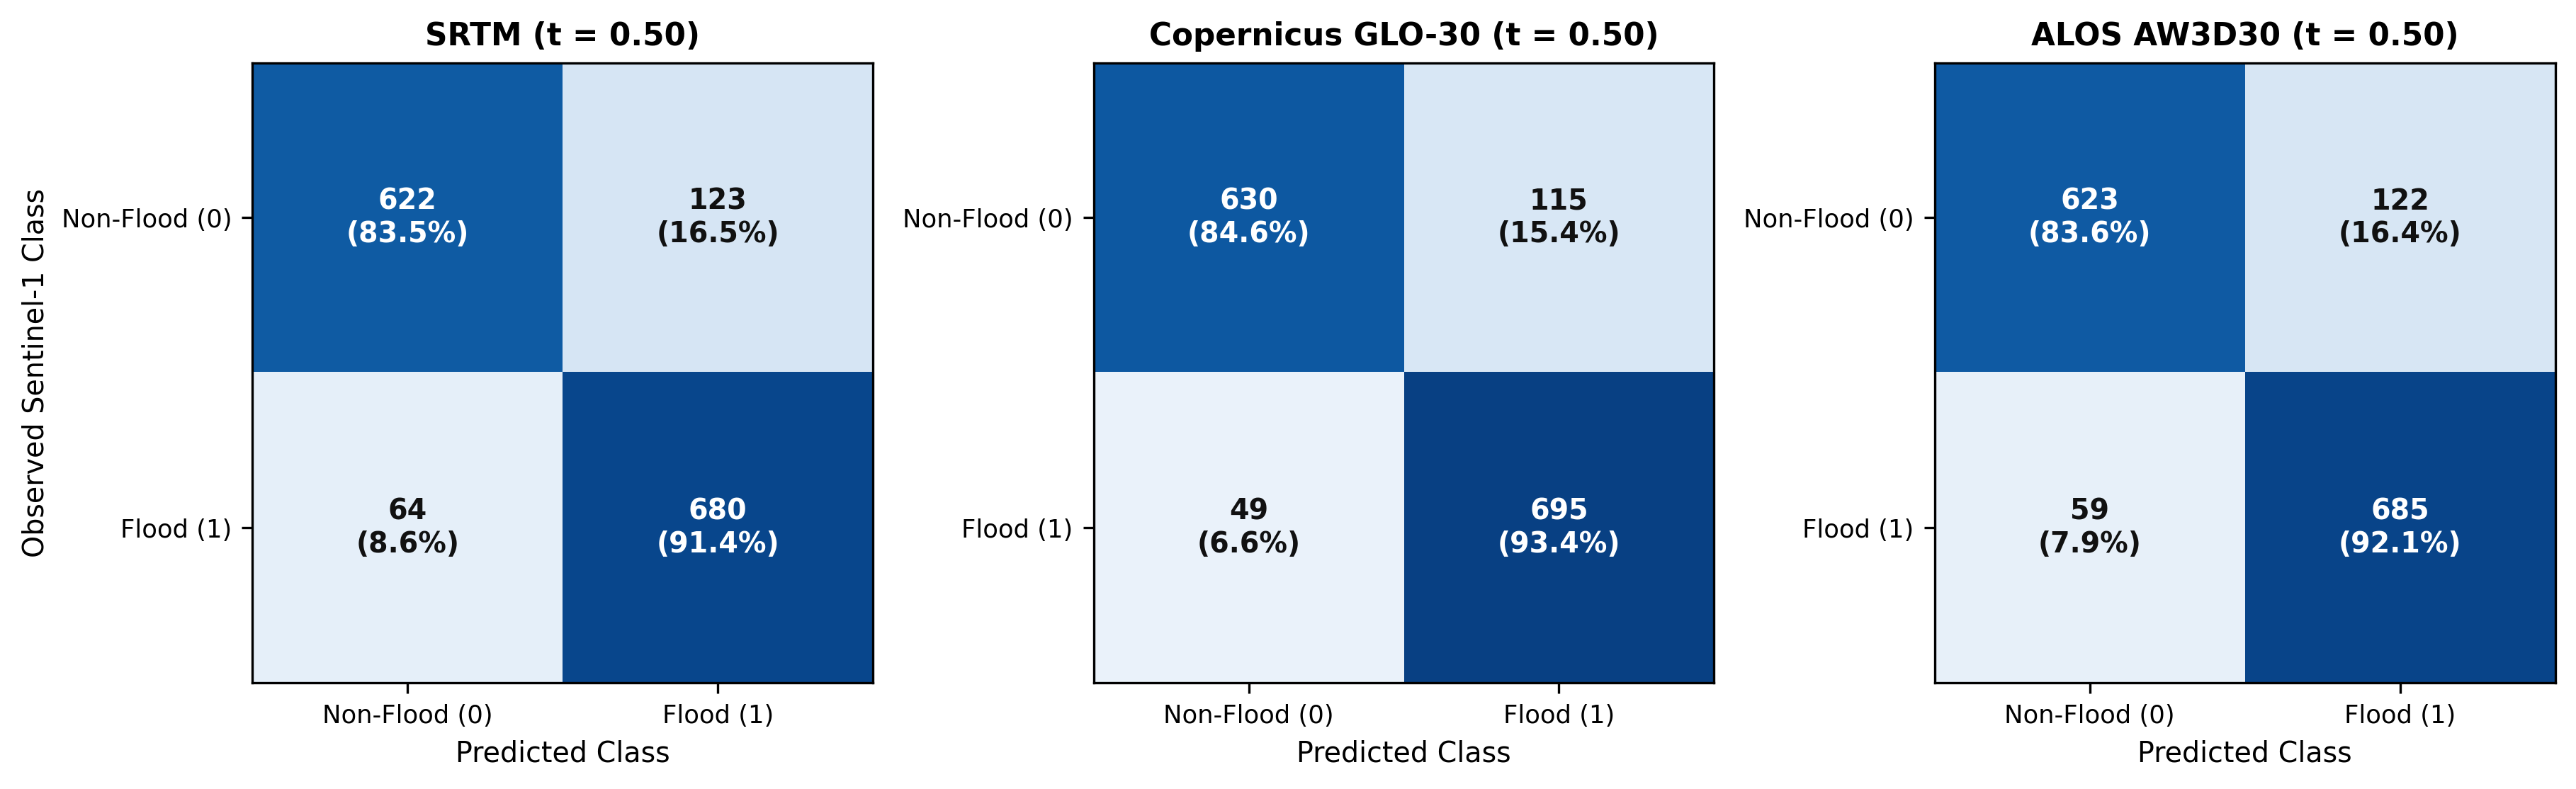
\includegraphics[width=0.92\textwidth,height=0.30\textheight,keepaspectratio]{figures/fig_confusion_matrices.png}
\caption[Matriks konfusi pada data uji holdout]{Matriks konfusi pada data uji \textit{holdout} ($n_{\text{uji}} = 1.489$; ambang $t = 0{,}50$) untuk SRTM, Copernicus DEM GLO-30, dan ALOS AW3D30.}
\label{fig:cm}
\end{figure}

\subsection{Perbandingan Performa}

Berdasarkan hasil evaluasi pada Tabel~\ref{tab:metrik-holdout} dan
Gambar~\ref{fig:roc}, ketiga produk elevasi menghasilkan kinerja
klasifikasi yang tinggi dengan urutan peringkat yang konsisten, yaitu
Copernicus DEM GLO-30 di atas ALOS AW3D30 dan SRTM, meskipun selisih
antarproduk relatif kecil (rentang ROC-AUC sekitar $0{,}008$). Mengingat
pembagian data secara acak berpotensi menghasilkan estimasi yang terlalu
optimistis akibat autokorelasi spasial \citep{roberts2017}, kemampuan
generalisasi spasial model diuji lebih lanjut menggunakan validasi silang
spasial 4-\textit{fold} (\textit{4-fold spatial cross-validation}). Pada skema
ini, wilayah kajian dibagi ke dalam 16 blok berbasis kuantil bujur dan
lintang. Setiap \textit{fold} melatih model pada 12 blok dan menguji kinerja
prediksi probabilitas pada 4 blok yang dipisahkan. Hasil validasi silang
spasial disajikan pada Tabel~\ref{tab:spatial-cv}.

\begin{figure}[!htbp]
\centering
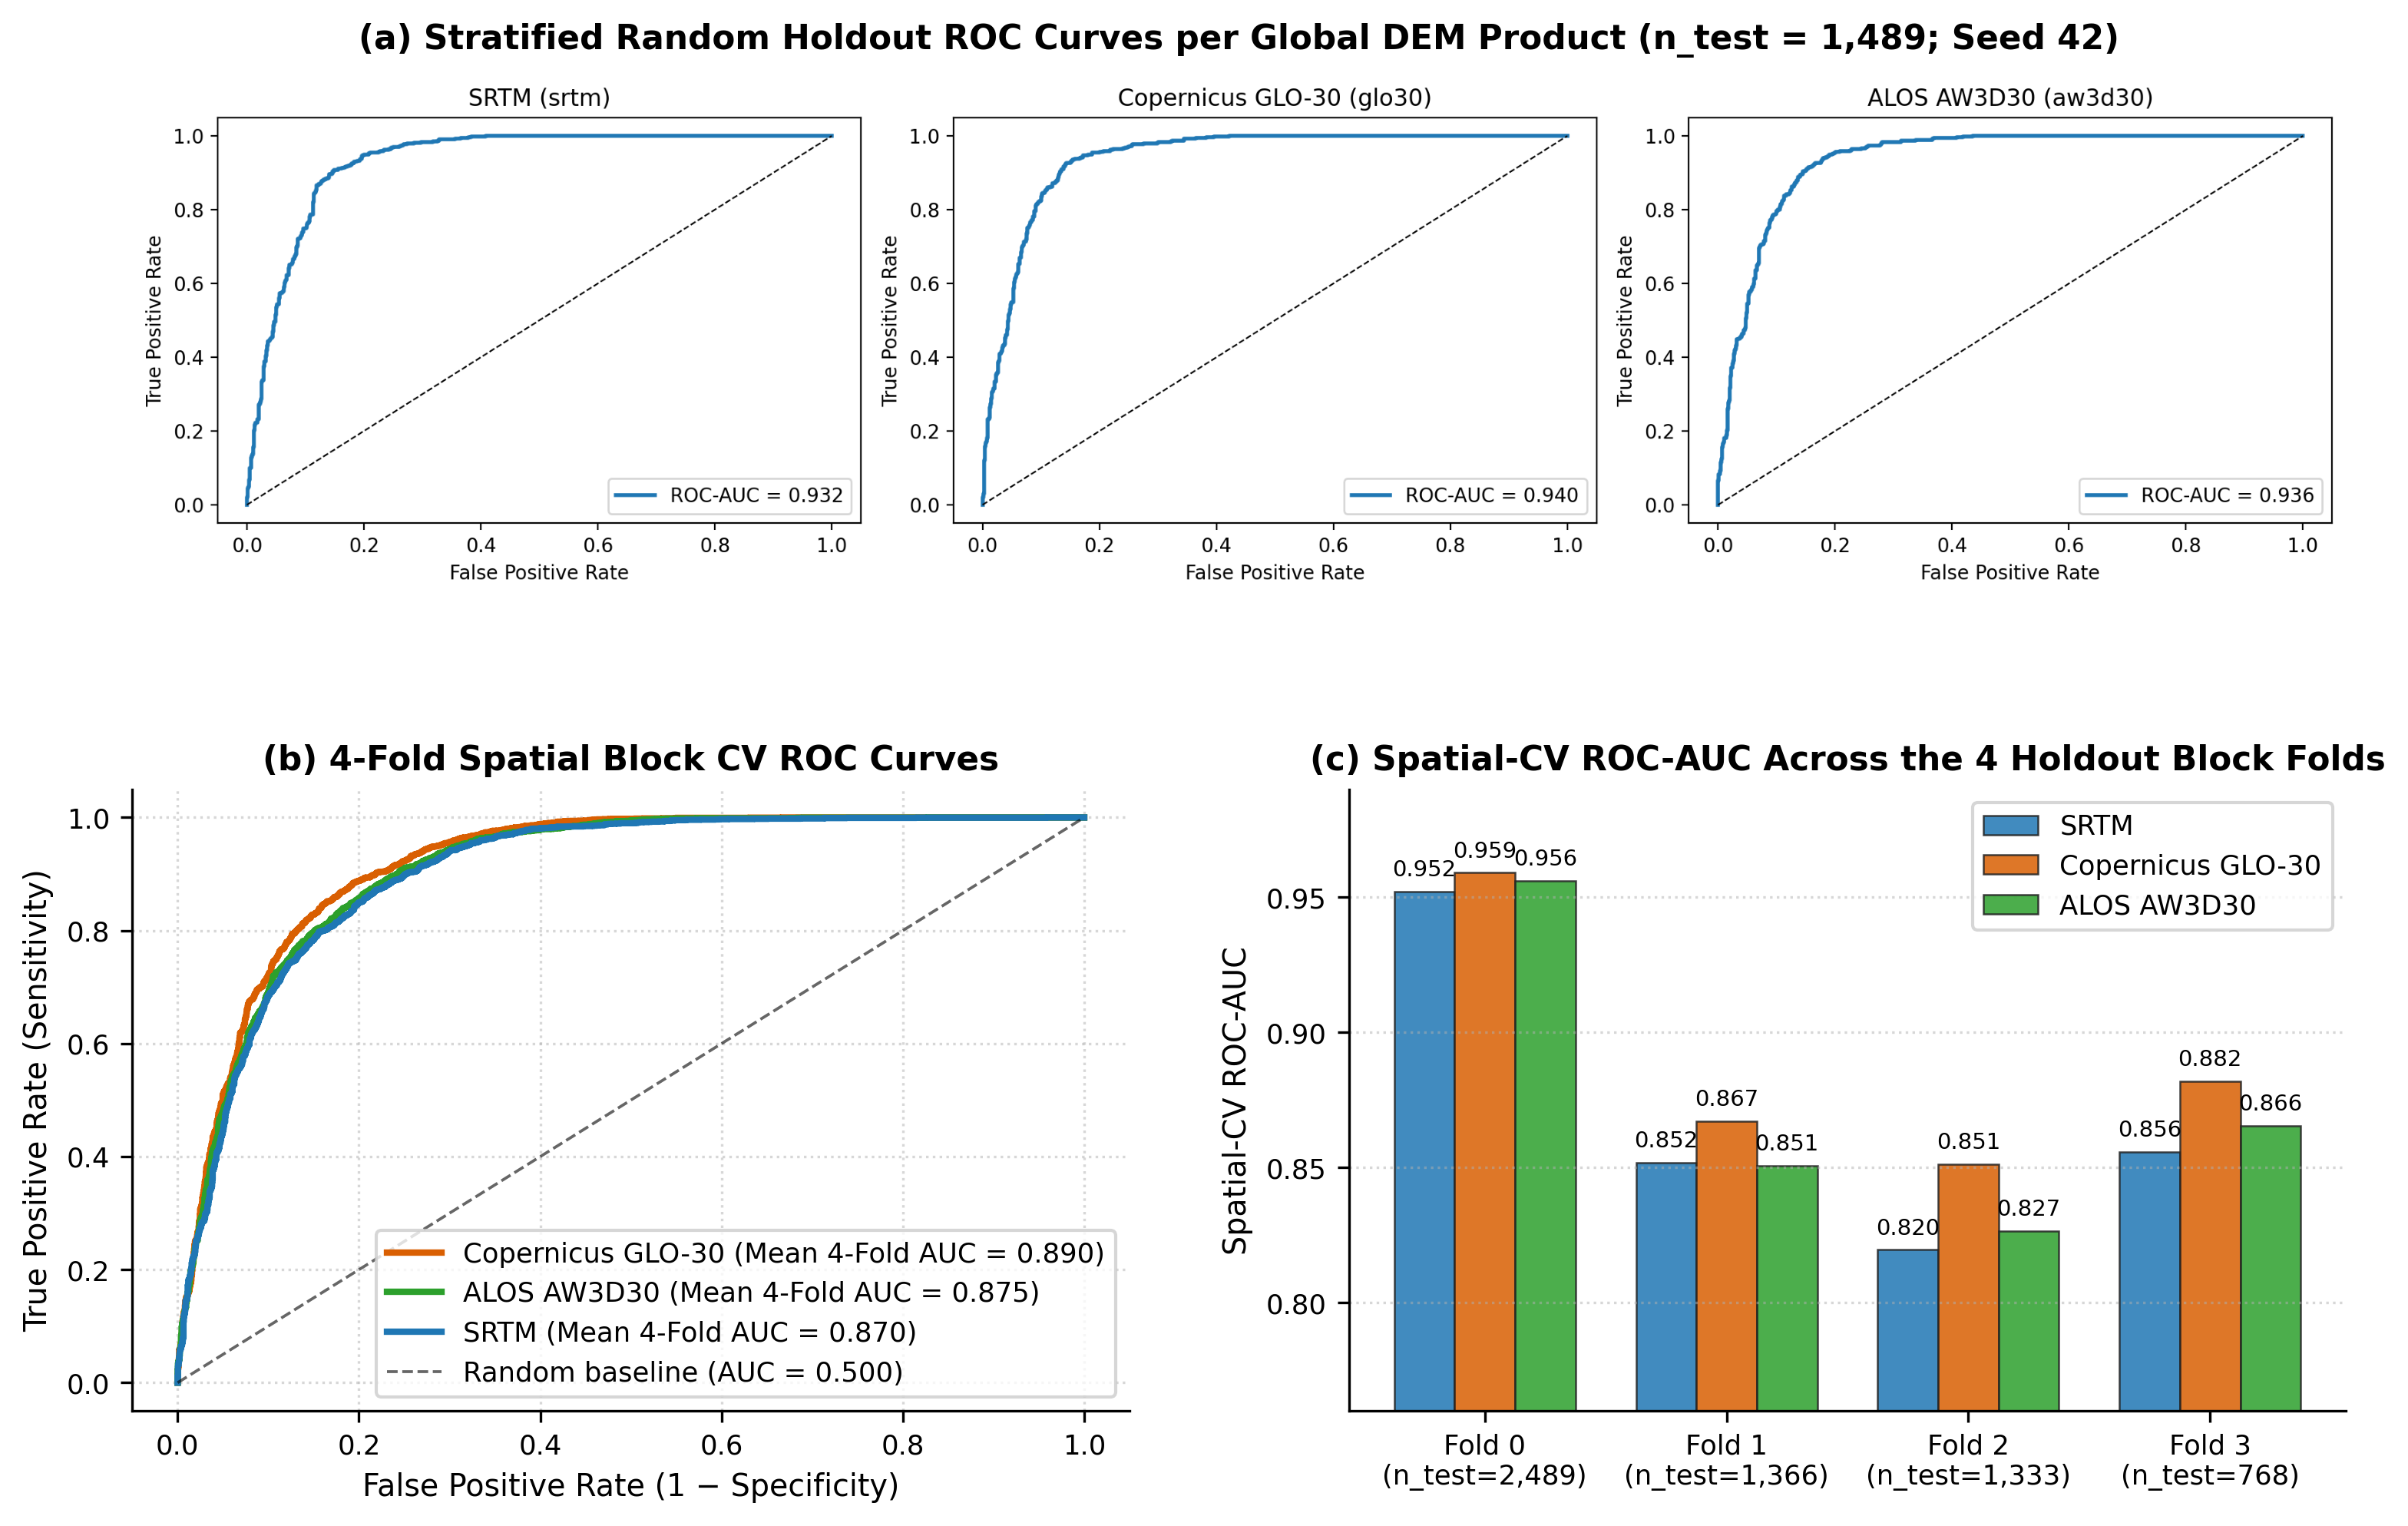
\includegraphics[width=0.92\textwidth,height=0.42\textheight,keepaspectratio]{figures/fig_roc.png}
\caption[Kurva dan metrik ROC lintas skema evaluasi]{Kurva dan metrik ROC lintas skema evaluasi: (a) kurva ROC \textit{holdout} acak terstratifikasi ($n_{\text{uji}} = 1.489$); (b) kurva ROC gabungan validasi silang spasial 4-\textit{fold}; dan (c) perbandingan ROC-AUC per \textit{fold} spasial.}
\label{fig:roc}
\end{figure}

\begin{table}[!htbp]
\small
\centering
\caption[Hasil validasi silang spasial 4-fold lintas 16 blok kuantil]{Hasil validasi silang spasial 4-\textit{fold} lintas 16 blok kuantil koordinat (\textit{seed} = 42; rincian per \textit{fold} dan rata-rata lintas \textit{fold}).}
\label{tab:spatial-cv}
\begin{adjustbox}{max width=\textwidth}
\begin{tabular}{c c c c l cccccc}
\toprule
\textbf{Fold} & \textbf{Blok Uji} & $\boldsymbol{n_{\text{latih}}}$ & $\boldsymbol{n_{\text{uji}}}$ & \textbf{Konfigurasi DEM} & $\textbf{AUC}_{\textbf{prob}}$ & $\textbf{AUC}_{\textbf{biner}}$ & \textbf{Akurasi} & \textbf{Presisi} & \textbf{Recall} & \textbf{F1-Score} \\
\midrule
0 & $\{0, 1, 5, 14\}$ & 3.467 & 2.489 & SRTM & 0,9521 & 0,8667 & 0,8734 & 0,8755 & 0,8203 & 0,8470 \\
  & & & & Copernicus GLO-30 & \textbf{0,9591} & \textbf{0,9047} & \textbf{0,9052} & 0,8797 & \textbf{0,9012} & \textbf{0,8903} \\
  & & & & ALOS AW3D30 & 0,9562 & 0,8870 & 0,8911 & \textbf{0,8830} & 0,8589 & 0,8708 \\
\midrule
1 & $\{8, 9, 11, 13\}$ & 4.590 & 1.366 & SRTM & 0,8519 & 0,7890 & 0,8302 & 0,8573 & \textbf{0,9014} & 0,8788 \\
  & & & & Copernicus GLO-30 & \textbf{0,8673} & \textbf{0,8119} & \textbf{0,8360} & \textbf{0,8816} & 0,8778 & \textbf{0,8797} \\
  & & & & ALOS AW3D30 & 0,8508 & 0,7891 & 0,8184 & 0,8655 & 0,8692 & 0,8674 \\
\midrule
2 & $\{2, 4, 7, 15\}$ & 4.623 & 1.333 & SRTM & 0,8197 & 0,7279 & 0,7374 & \textbf{0,6939} & 0,6691 & 0,6812 \\
  & & & & Copernicus GLO-30 & \textbf{0,8514} & \textbf{0,7523} & \textbf{0,7539} & 0,6928 & \textbf{0,7424} & \textbf{0,7168} \\
  & & & & ALOS AW3D30 & 0,8265 & 0,7177 & 0,7269 & 0,6796 & 0,6601 & 0,6697 \\
\midrule
3 & $\{3, 6, 10, 12\}$ & 5.188 & 768 & SRTM & 0,8559 & 0,7694 & 0,7669 & 0,8161 & 0,7447 & 0,7787 \\
  & & & & Copernicus GLO-30 & \textbf{0,8820} & \textbf{0,7991} & \textbf{0,8008} & \textbf{0,8214} & \textbf{0,8156} & \textbf{0,8185} \\
  & & & & ALOS AW3D30 & 0,8655 & 0,7806 & 0,7812 & 0,8102 & 0,7872 & 0,7986 \\
\midrule
\multicolumn{4}{l}{\textbf{Rata-Rata Lintas 4 Fold Spasial}} & SRTM & 0,8699 & 0,7883 & 0,8020 & 0,8107 & 0,7839 & 0,7964 \\
\multicolumn{4}{l}{} & Copernicus GLO-30 & \textbf{0,8899} & \textbf{0,8170} & \textbf{0,8240} & \textbf{0,8189} & \textbf{0,8343} & \textbf{0,8263} \\
\multicolumn{4}{l}{} & ALOS AW3D30 & 0,8747 & 0,7936 & 0,8044 & \textbf{0,8096} & 0,7939 & 0,8016 \\
\bottomrule
\end{tabular}
\end{adjustbox}
\end{table}

Signifikansi perbedaan kinerja antarproduk elevasi pada skema validasi spasial
diuji menggunakan prosedur \textit{bootstrap} dua tingkat. Pengujian utama
menerapkan \textit{block bootstrap} pada 16 blok kuantil bujur dan lintang
yang sama dengan skema validasi silang spasial melalui pengambilan sampel
ulang blok dengan pengembalian sebanyak 1.000 iterasi, di mana nilai ROC-AUC
setiap pasangan produk dihitung pada sampel ulang yang identik. Rata-rata
ROC-AUC pada sampel ulang blok tercatat sebesar $0{,}894$ untuk SRTM,
$0{,}910$ untuk Copernicus DEM GLO-30, dan $0{,}899$ untuk ALOS AW3D30.
Selisih performa antara SRTM dan Copernicus DEM GLO-30 adalah
$\Delta\text{AUC}_{\text{SRTM}-\text{GLO-30}} = -0{,}0155$ dengan selang
kepercayaan 95\% $[-0{,}0250;\,-0{,}0072]$, sedangkan selisih antara
Copernicus DEM GLO-30 dan ALOS AW3D30 adalah
$\Delta\text{AUC}_{\text{GLO-30}-\text{AW3D30}} = +0{,}0108$ dengan selang
kepercayaan $[+0{,}0041;\,+0{,}0198]$. Kedua selang kepercayaan tersebut tidak
memuat nilai nol, sehingga keunggulan Copernicus DEM GLO-30 konsisten pada
sampel ulang blok dalam eksperimen ini, meskipun besaran selisihnya relatif
kecil (maksimal sekitar $0{,}016$). Sebaliknya, selisih antara SRTM dan ALOS
AW3D30 sebesar $\Delta\text{AUC}_{\text{SRTM}-\text{AW3D30}} = -0{,}0047$
$[-0{,}0096;\,+0{,}0013]$ masih memuat nilai nol, sehingga peringkat keduanya
pada skema spasial ini belum dapat dipisahkan. Sebagai pembanding, pengujian
\textit{bootstrap} pada tingkat piksel menghasilkan selang kepercayaan yang
lebih sempit dengan nilai $|\Delta\text{AUC}|$ antara Copernicus DEM GLO-30
dan SRTM sebesar $0{,}0141$ $[0{,}0109;\,0{,}0173]$. Interval ini dilaporkan
dengan catatan bahwa piksel digunakan sebagai unit resampling ketika piksel
bersebelahan cenderung bersifat dependen, sehingga selang yang lebih sempit
tersebut tidak menjadikan dasar inferensi utama.

Ketahanan (\textit{robustness}) hasil pemodelan terhadap variasi pembangkit
acak diuji dengan menjalankan ulang keseluruhan alur pemodelan sejak tahap
awal menggunakan lima nilai \textit{seed} yang berbeda (42, 100, 2024, 7, dan
99). Pada setiap \textit{seed}, pengambilan sampel di Google Earth Engine,
ekstraksi fitur prediktor, pembagian data acak, serta validasi silang spasial
diulang secara menyeluruh. Pengujian multi-\textit{seed} beserta analisis
\textit{block bootstrap} tersebut dijalankan pada alur pemodelan yang sama
dengan analisis lainnya, kecuali analisis pembanding yang memakai sampel dan
pembagian data penelitian acuan. Hasil pada Tabel~\ref{tab:multiseed} memperlihatkan bahwa
Copernicus DEM GLO-30 menempati peringkat tertinggi secara konsisten pada
kelima nilai \textit{seed}, baik pada evaluasi \textit{holdout} maupun validasi
silang spasial. Urutan lengkap dengan ALOS AW3D30 di atas SRTM berlaku pada
validasi silang spasial, tetapi pada dua dari lima evaluasi \textit{holdout}
(\textit{seed}~42 dan 100) SRTM mencatatkan AUC sedikit lebih tinggi daripada
ALOS AW3D30 dengan selisih tidak lebih dari $0{,}0006$. Pada validasi silang spasial, kinerja ALOS
AW3D30 tercatat di atas SRTM pada kelima \textit{seed}
($\Delta\text{AUC}_{\text{SRTM}-\text{AW3D30}} = -0{,}0079 \pm 0{,}0034$),
sedangkan pada evaluasi \textit{holdout} keduanya menunjukkan kinerja yang
nyaris setara ($\Delta\text{AUC}_{\text{SRTM}-\text{AW3D30}} = -0{,}0012 \pm
0{,}0021$). Perbedaan nilai antar skema evaluasi ini menunjukkan bahwa ketepatan
pemisahan peringkat ALOS AW3D30 dan SRTM bergantung pada skema evaluasi yang
dipakai. Secara keseluruhan, selisih performa antarproduk elevasi tetap
kecil dan stabil lintas \textit{seed}, dengan nilai
$\Delta\text{AUC}_{\text{GLO-30}-\text{AW3D30}} = +0{,}0070 \pm 0{,}0027$ dan
$\Delta\text{AUC}_{\text{SRTM}-\text{GLO-30}} = -0{,}0082 \pm 0{,}0048$ pada
skema \textit{holdout}. Sebagai catatan skema fitur, representasi dummy tutupan
lahan mengikuti kelas ESA WorldCover yang benar-benar hadir pada sampel
masing-masing \textit{seed}: kelas~20 (semak belukar) hadir pada sampel
\textit{seed}~100, 2024, dan 7 sehingga jumlah input efektif membesar menjadi
25 pada \textit{seed} tersebut, sedangkan sampel utama serta \textit{seed}~42
dan 99 memakai 24 prediktor. Kontras antarproduk dalam satu \textit{seed}
tetap dihitung berpasangan sehingga pembandingan antarproduk tidak terganggu
perbedaan ini.

\begin{table}[!htbp]
\small
\centering
\caption[Perbandingan selisih ROC-AUC block vs bootstrap piksel]{Perbandingan $\Delta\text{AUC}$ berpasangan pada \textit{block bootstrap} 16 blok vs.\ \textit{bootstrap} piksel, serta kestabilan lintas lima \textit{seed} ($\{7, 42, 99, 100, 2024\}$).}
\label{tab:bootstrap}
\begin{adjustbox}{max width=\textwidth}
\begin{tabular}{l rrrr rrr rr}
\toprule
& \multicolumn{4}{c}{\textbf{Block Bootstrap 16 Blok ($B=1.000$)}} & \multicolumn{3}{c}{\textbf{Bootstrap Piksel ($B=1.000$)}} & \multicolumn{2}{c}{\textbf{Replikasi 5-Seed ($\text{Mean} \pm \text{SD}$)}} \\
\cmidrule(lr){2-5} \cmidrule(lr){6-8} \cmidrule(lr){9-10}
\textbf{Pasangan Produk DEM} & $\boldsymbol{\Delta}\textbf{AUC}$ & \textbf{SD} & \textbf{CI 95\%} & \textbf{Tanpa 0?} & $\boldsymbol{\Delta}\textbf{AUC}$ & \textbf{CI 95\%} & \textbf{Tanpa 0?} & \textbf{Holdout $\boldsymbol{\Delta}$AUC} & \textbf{Spatial-CV $\boldsymbol{\Delta}$AUC} \\
\midrule
SRTM minus GLO-30 & $-0{,}0155$ & 0,0047 & $[-0{,}0250; -0{,}0072]$ & Ya & $-0{,}0141$ & $[-0{,}0173; -0{,}0109]$ & Ya & $-0{,}0082 \pm 0{,}0048$ & $-0{,}0200 \pm 0{,}0039$ \\
SRTM minus AW3D30 & $-0{,}0047$ & 0,0028 & $[-0{,}0096; +0{,}0013]$ & Tidak (Marginal) & $-0{,}0048$ & $[-0{,}0074; -0{,}0023]$ & Ya (Semu) & $-0{,}0012 \pm 0{,}0021$ & $-0{,}0079 \pm 0{,}0034$ \\
GLO-30 minus AW3D30 & $+0{,}0108$ & 0,0042 & $[+0{,}0041; +0{,}0198]$ & Ya & $+0{,}0094$ & $[+0{,}0063; +0{,}0124]$ & Ya & $+0{,}0070 \pm 0{,}0027$ & $+0{,}0121 \pm 0{,}0055$ \\
\bottomrule
\end{tabular}
\end{adjustbox}
\end{table}

\begin{figure}[!htbp]
\centering
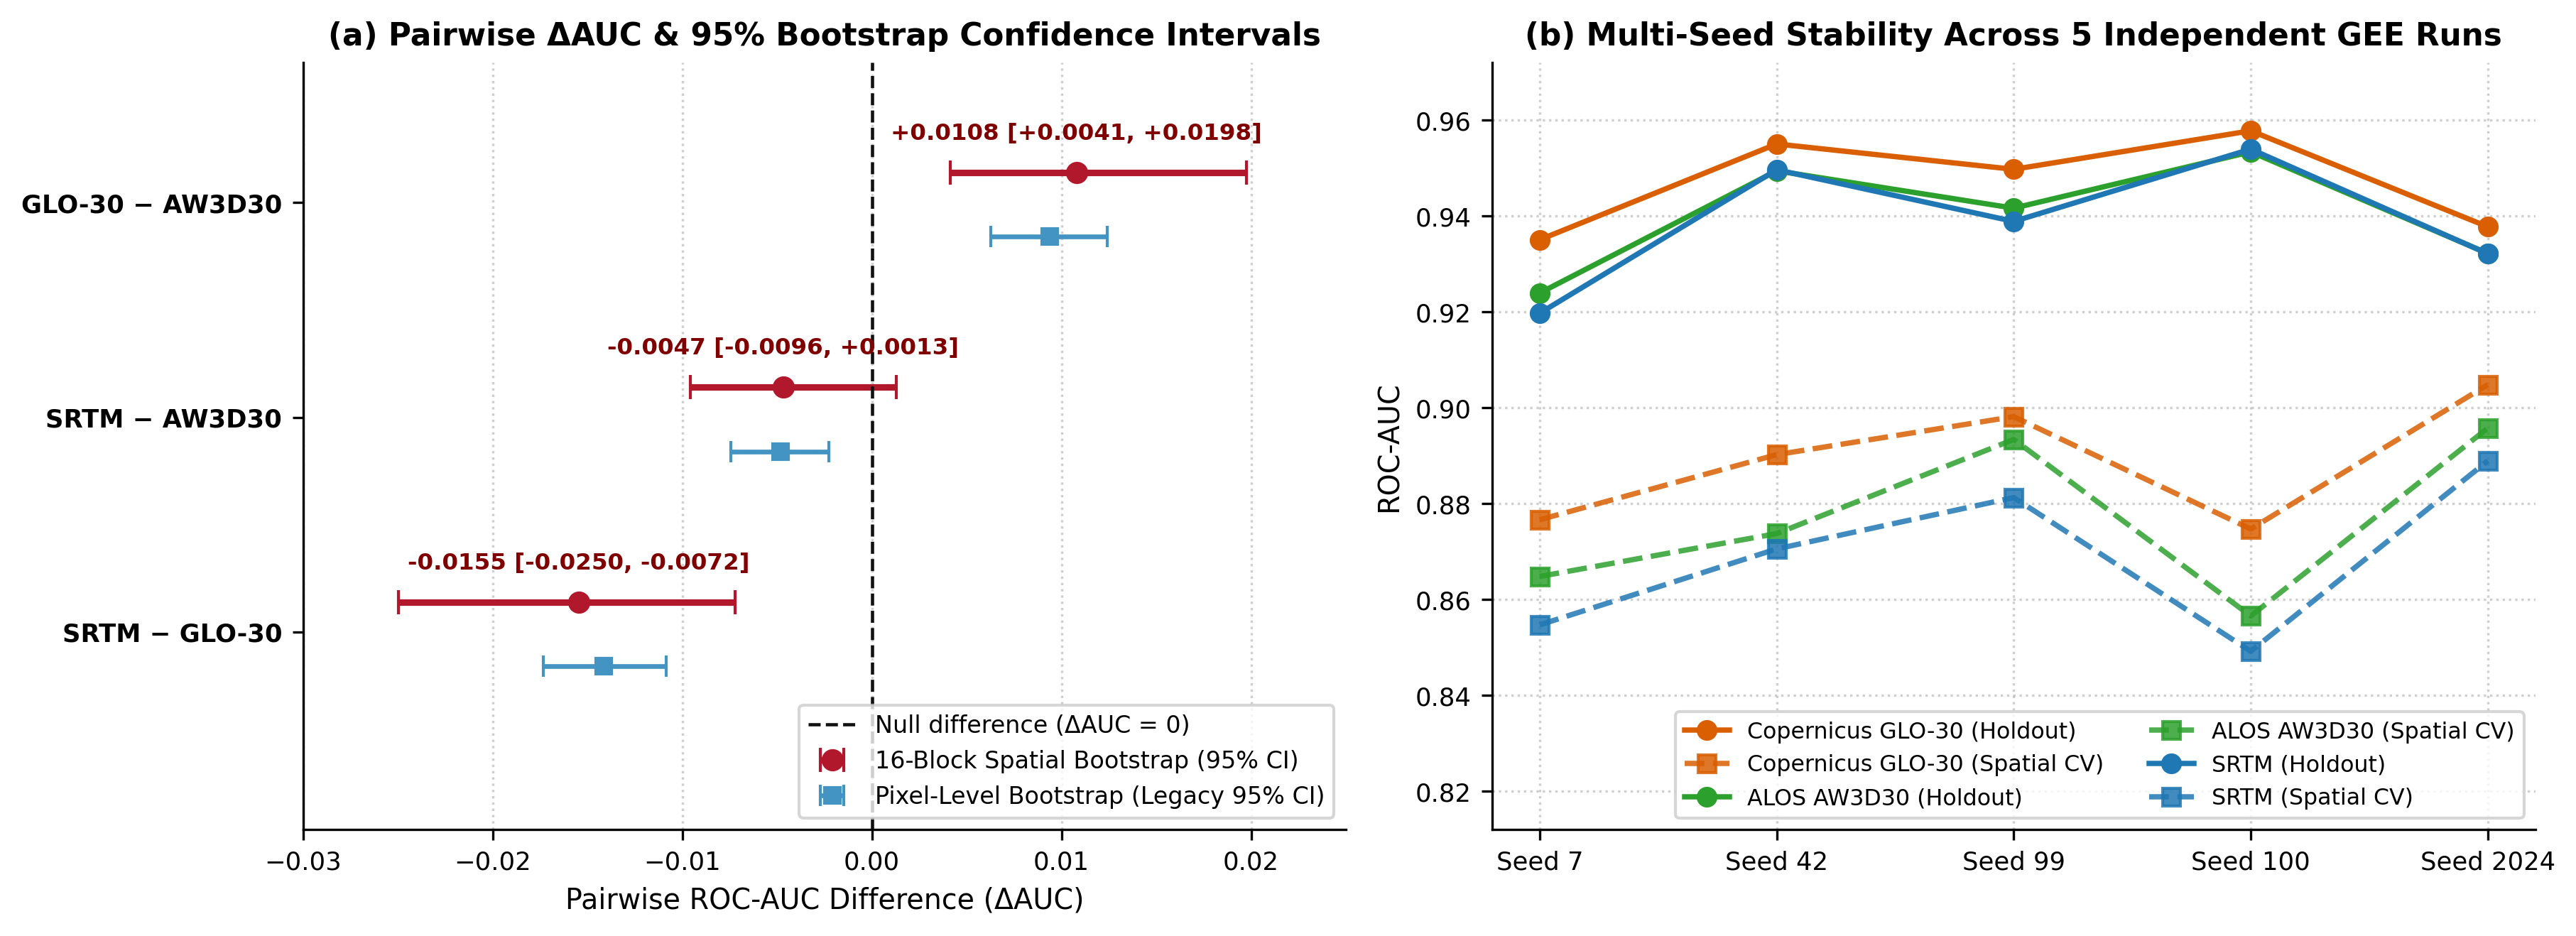
\includegraphics[width=0.92\textwidth,height=0.36\textheight,keepaspectratio]{figures/fig_bootstrap_multiseed.png}
\caption[Inferensi block bootstrap dan ketahanan multi-seed]{Inferensi statistik dan ketahanan multi-\textit{seed}: (a) selang kepercayaan 95\% $\Delta\text{AUC}$ pada \textit{block bootstrap} 16 blok vs.\ \textit{bootstrap} piksel; (b) stabilitas ROC-AUC lintas lima \textit{seed} independen ($7, 42, 99, 100, 2024$).}
\label{fig:bootstrap}
\end{figure}

\begin{table}[!htbp]
\small
\centering
\caption[Evaluasi ketahanan multi-seed lintas lima nilai seed]{Evaluasi ketahanan multi-\textit{seed}: nilai per \textit{seed} serta rata-rata $\pm$ simpangan baku lintas lima nilai \textit{seed} (42, 100, 2024, 7, dan 99).}
\label{tab:multiseed}
\begin{adjustbox}{max width=\textwidth}
\begin{tabular}{l ccccc c c}
\toprule
& \multicolumn{5}{c}{\textbf{ROC-AUC Validasi Spasial per Seed (ROC-AUC Holdout dalam Kurung)}} & \multicolumn{2}{c}{\textbf{Rata-Rata $\pm$ SD (5 Seed)}} \\
\cmidrule(lr){2-6} \cmidrule(lr){7-8}
\textbf{Konfigurasi DEM} & \textbf{Seed 7} & \textbf{Seed 42} & \textbf{Seed 99} & \textbf{Seed 100} & \textbf{Seed 2024} & \textbf{Holdout AUC} & \textbf{Spatial-CV AUC} \\
\midrule
SRTM & 0,8547 (0,9197) & 0,8706 (0,9497) & 0,8813 (0,9389) & 0,8492 (0,9540) & 0,8890 (0,9322) & $0{,}9389 \pm 0{,}0138$ & $0{,}8689 \pm 0{,}0169$ \\
Copernicus GLO-30 & \textbf{0,8767} (\textbf{0,9351}) & \textbf{0,8902} (\textbf{0,9551}) & \textbf{0,8982} (\textbf{0,9498}) & \textbf{0,8747} (\textbf{0,9578}) & \textbf{0,9049} (\textbf{0,9378}) & $\mathbf{0{,}9471 \pm 0{,}0102}$ & $\mathbf{0{,}8889 \pm 0{,}0132}$ \\
ALOS AW3D30 & 0,8648 (0,9240) & 0,8738 (0,9495) & 0,8934 (0,9417) & 0,8566 (0,9534) & 0,8958 (0,9322) & $0{,}9402 \pm 0{,}0121$ & $0{,}8769 \pm 0{,}0173$ \\
\bottomrule
\end{tabular}
\end{adjustbox}
\end{table}

Untuk menghubungkan temuan ini dengan penelitian acuan \citep{hakim2026}, alur
pemodelan juga diuji menggunakan 1.870 titik sampel dan pembagian data
latih-uji yang identik dengan penelitian tersebut melalui ekstraksi ulang
seluruh variabel prediktor. Konfigurasi SRTM menghasilkan nilai ROC-AUC
sebesar $0{,}802$, lebih rendah dibandingkan nilai acuan sebesar $0{,}852$
(selisih sekitar $0{,}05$), diikuti oleh Copernicus DEM GLO-30 sebesar
$0{,}795$ dan ALOS AW3D30 sebesar $0{,}792$. Hasil ini menunjukkan bahwa alur
pemodelan mampu mendekati tingkat kinerja acuan secara kasar, namun urutan
peringkat pada pengujian pembanding ini tidak sama dengan eksperimen utama.
Urutan peringkat antarproduk karenanya bergantung pada himpunan sampel yang
dipakai, temuan yang memperkuat keterbatasan pada Subbab~4.8 mengenai
sensitivitas hasil terhadap desain sampel. Di samping itu, perbandingan
dengan eksperimen awal pada domain terbatas di sekitar perairan kembali
menegaskan sensitivitas model terhadap desain sampel
non-banjir, di mana ketiga produk hanya memperoleh nilai ROC-AUC validasi
silang spasial sekitar $0{,}70$, atau berbeda sekitar $0{,}17$ dibandingkan
hasil pemodelan pada seluruh wilayah kajian.

\subsection{Analisis Sensitivitas Spasial}

Evaluasi sensitivitas spasial dilakukan melalui perbandingan piksel demi
piksel pada seluruh wilayah penelitian (sekitar $1{,}4$~juta piksel) di
antara ketiga peta probabilitas \textit{flood susceptibility}. Ringkasan hasil
perbandingan disajikan pada Tabel~\ref{tab:sensitivitas}. Pembahasan
berikut dibatasi pada ketiga peta dari eksperimen utama. Pada perbandingan
antarpeta tersebut, pasangan SRTM
dan ALOS AW3D30 menunjukkan
tingkat kemiripan spasial tertinggi, sedangkan pasangan yang melibatkan
Copernicus DEM GLO-30 menghasilkan perbedaan spasial yang lebih besar.

\begin{table}[!htbp]
\small
\centering
\caption[Distribusi luas kelas kerawanan banjir dan sensitivitas spasial]{Distribusi luas kelas kerawanan banjir ($\text{km}^2$ dan \%) serta ringkasan sensitivitas spasial berpasangan pasca-masking AOI di wilayah Semarang--Demak.}
\label{tab:sensitivitas}
\begin{adjustbox}{max width=\textwidth}
\begin{tabular}{l rrr rrr l cc}
\toprule
& \multicolumn{3}{c}{\textbf{Luas Area Terpetakan ($\text{km}^2$)}} & \multicolumn{3}{c}{\textbf{Proporsi Wilayah (\%)}} & & \multicolumn{2}{c}{\textbf{Sensitivitas Berpasangan}} \\
\cmidrule(lr){2-4} \cmidrule(lr){5-7} \cmidrule(lr){9-10}
\textbf{Kelas Kerawanan (Interval Probabilitas)} & \textbf{SRTM} & \textbf{GLO-30} & \textbf{AW3D30} & \textbf{SRTM} & \textbf{GLO-30} & \textbf{AW3D30} & \textbf{Pasangan DEM} & $\boldsymbol{\overline{|\Delta p|}}$ & \textbf{Agreement (\%)} \\
\midrule
Kelas 1: Sangat Rendah ($p \le 0{,}20$) & 756,71 & 822,64 & 772,46 & 58,22 & 63,29 & 60,03 & SRTM vs.\ GLO-30 & 0,0556 & 79,36\% \\
Kelas 2: Rendah ($0{,}20 < p \le 0{,}40$) & 233,13 & 189,85 & 222,06 & 17,94 & 14,61 & 17,26 & SRTM vs.\ AW3D30 & 0,0371 & 84,27\% \\
Kelas 3: Sedang ($0{,}40 < p \le 0{,}60$) & 114,08 & 98,47 & 108,18 & 8,78 & 7,58 & 8,41 & GLO-30 vs.\ AW3D30 & 0,0483 & 81,52\% \\
Kelas 4: Tinggi ($0{,}60 < p \le 0{,}80$) & 95,34 & 79,25 & 88,16 & 7,33 & 6,10 & 6,85 & & & \\
Kelas 5: Sangat Tinggi ($p > 0{,}80$) & 100,58 & 109,63 & 95,93 & 7,74 & 8,43 & 7,46 & & & \\
\midrule
\textbf{Total Luas Valid AOI} & \textbf{1.299,84} & \textbf{1.299,84} & \textbf{1.286,79} & \textbf{100,00} & \textbf{100,00} & \textbf{100,00} & & & \\
\bottomrule
\end{tabular}
\end{adjustbox}
\end{table}

\begin{figure}[!htbp]
\centering
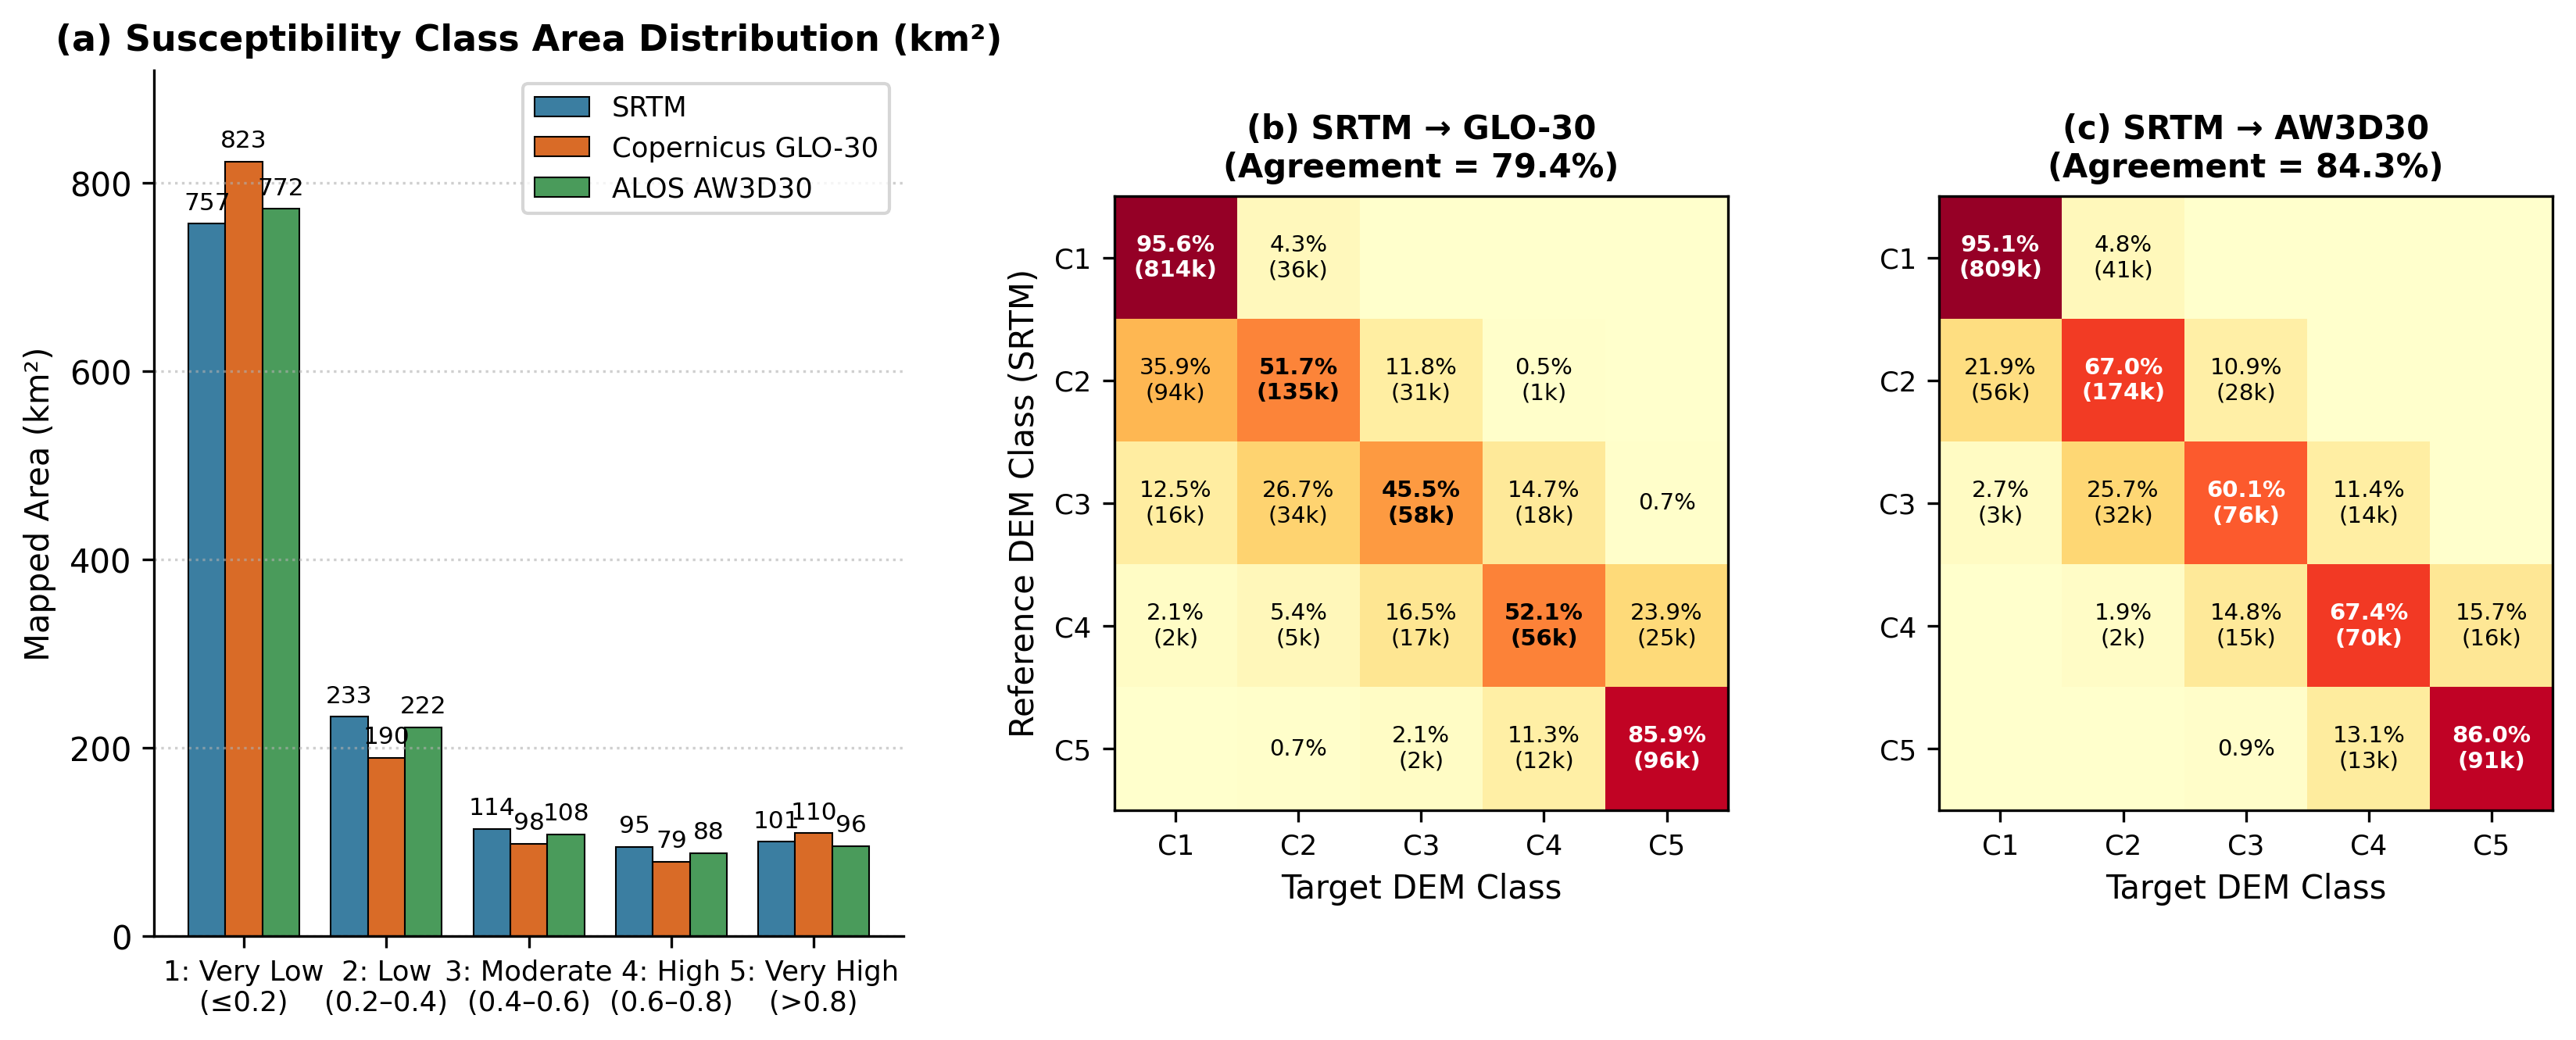
\includegraphics[width=0.92\textwidth,height=0.34\textheight,keepaspectratio]{figures/fig_spatial_sensitivity.png}
\caption[Sensitivitas spasial dan matriks transisi kelas]{Sensitivitas spasial antarpeta kerawanan banjir: (a) luas area per kelas kerawanan ($\text{km}^2$); (b) matriks transisi kelas SRTM ke Copernicus DEM GLO-30; dan (c) matriks transisi kelas SRTM ke ALOS AW3D30.}
\label{fig:spatial-sensitivity}
\end{figure}

Perbedaan distribusi spasial antarpeta terutama terjadi pada kedua kelas
kerawanan ekstrem. Luas wilayah yang tergolong ke dalam kelas~5 (kerawanan
sangat tinggi) tercatat sebesar $100{,}6\text{ km}^2$ pada SRTM,
$109{,}6\text{ km}^2$ pada Copernicus DEM GLO-30, dan $95{,}9\text{ km}^2$
pada ALOS AW3D30. Sementara itu, luas wilayah pada kelas~1 (kerawanan sangat
rendah) masing-masing adalah $756{,}7\text{ km}^2$ pada SRTM,
$822{,}6\text{ km}^2$ pada Copernicus DEM GLO-30, dan $772{,}5\text{ km}^2$
pada ALOS AW3D30. Pola tersebut menunjukkan bahwa Copernicus DEM GLO-30
cenderung menghasilkan sebaran distribusi probabilitas yang lebih lebar dengan
peningkatan luas pada kedua kelas ujung, sedangkan ALOS AW3D30 memiliki
distribusi yang mendekati SRTM pada kelas kerawanan rendah tetapi mencatat
cakupan yang paling sempit di antara ketiga produk pada kelas kerawanan
sangat tinggi. Berdasarkan
analisis matriks transisi antarkelas dari SRTM menuju Copernicus DEM GLO-30,
perpindahan piksel terbesar terjadi dari kelas~2 ke kelas~1 sebanyak
94.306~piksel dan dari kelas~1 ke kelas~2 sebanyak 36.869~piksel, diikuti oleh
transisi dari kelas~4 ke kelas~5 sebanyak 25.679~piksel. Sebaliknya,
perbandingan antara SRTM dan ALOS AW3D30 lebih didominasi oleh kesesuaian pada
kelas yang sama (elemen diagonal), seperti pada kelas~2 sebanyak
174.072~piksel dan pada kelas~5 sebanyak 91.194~piksel. Angka matriks
tersebut berasal dari reduksi server Google Earth Engine, sedangkan
Moran's I peta dihitung dari raster ter-ekspor. Jumlah piksel pada kedua
analisis tidak identik. Perbedaan registrasi grid dan kriteria piksel valid
perlu diperhatikan, tetapi kontribusinya terhadap selisih tersebut belum
dipisahkan. Luas kelas dan persentase kesesuaian pada tabel Subbab~4.5
merujuk pada reduksi GEE, bukan hitungan ulang raster lokal pasca-mask.
Nilainya sedikit berbeda pada kedua sumber tersebut. Karena itu, domain
masing-masing sumber harus dibedakan dan penyebut antaranalisis tidak
diasumsikan identik.

\subsection{Sensitivitas Berdasarkan Tutupan Lahan}

Hasil stratifikasi menggunakan peta tutupan lahan ESA WorldCover menunjukkan
bahwa tingkat sensitivitas spasial terhadap perubahan sumber produk elevasi
tidak bersifat seragam di seluruh jenis permukaan (Gambar~\ref{fig:agreement}).
Kelas tutupan
pohon (\textit{tree cover}) menunjukkan konsistensi spasial yang paling stabil
di seluruh pasangan produk elevasi, dengan tingkat kesesuaian kelas
(\textit{spatial agreement}) berkisar antara 95,6\% hingga 96,9\% dan
rata-rata selisih probabilitas ($|\Delta p|$) sebesar $0{,}011$ hingga
$0{,}021$, diikuti oleh kawasan terbangun (\textit{built-up}) dengan
kesesuaian kelas sebesar 87,2\% hingga 91,2\%. Sebaliknya, sensitivitas
tertinggi terkonsentrasi pada kelas semak belukar (\textit{shrubland}), lahan
terbuka atau vegetasi jarang (\textit{bare/sparse vegetation}), serta kawasan
mangrove. Pada kelas \textit{shrubland}, tingkat kesesuaian kelas turun hingga
mencapai 57,6\% pada pasangan Copernicus DEM GLO-30 dan ALOS AW3D30 serta
59,1\% pada pasangan SRTM dan Copernicus DEM GLO-30, dengan rata-rata
$|\Delta p|$ tertinggi sebesar $0{,}094$ pada pasangan SRTM dan Copernicus DEM
GLO-30. Pada pasangan produk yang melibatkan Copernicus DEM GLO-30, tingkat
kesesuaian kelas juga relatif rendah pada lahan terbuka atau vegetasi jarang
(63,1\% dan 68,6\%) serta kawasan mangrove (62,6\% hingga 62,8\%). Adapun
kelas badan air mencatat kesesuaian kelas berkisar antara 76,9\% dan 84,1\%,
sedangkan lahan basah (\textit{wetland}) berkisar antara 72,5\% dan 78,3\%,
sehingga kedua tipe permukaan ini berada pada rentang sensitivitas yang
lebih rendah dibandingkan kelas-kelas pada paragraf sebelumnya tetapi tetap
di bawah tingkat kesesuaian tutupan pohon dan kawasan terbangun.

\begin{table}[!htbp]
\small
\centering
\caption[Stratifikasi sensitivitas spasial berdasarkan kelas WorldCover]{Stratifikasi sensitivitas spasial berdasarkan kelas tutupan lahan ESA WorldCover v200 pada ketiga pasangan produk elevasi.}
\label{tab:worldcover}
\begin{adjustbox}{max width=\textwidth}
\begin{tabular}{cl ccc ccc ccc}
\toprule
& & \multicolumn{3}{c}{\textbf{Rerata Selisih Probabilitas $\boldsymbol{\overline{|\Delta p|}}$}} & \multicolumn{3}{c}{\textbf{Tingkat Kesesuaian Kelas (\%)}} & \multicolumn{3}{c}{\textbf{Proporsi Berubah Kelas (\%)}} \\
\cmidrule(lr){3-5} \cmidrule(lr){6-8} \cmidrule(lr){9-11}
\textbf{Kode} & \textbf{Kelas WorldCover} & \textbf{SRTM--GLO30} & \textbf{SRTM--AW3D30} & \textbf{GLO30--AW3D30} & \textbf{SRTM--GLO30} & \textbf{SRTM--AW3D30} & \textbf{GLO30--AW3D30} & \textbf{SRTM--GLO30} & \textbf{SRTM--AW3D30} & \textbf{GLO30--AW3D30} \\
\midrule
10 & Tutupan pohon & 0,0210 & 0,0113 & 0,0170 & \textbf{95,61} & \textbf{96,78} & \textbf{96,87} & 4,39 & 3,22 & 3,13 \\
50 & Kawasan terbangun & 0,0514 & 0,0290 & 0,0373 & 87,19 & 91,18 & 90,77 & 12,81 & 8,82 & 9,23 \\
30 & Padang rumput & 0,0538 & 0,0300 & 0,0484 & 78,25 & 86,65 & 80,86 & 21,75 & 13,35 & 19,14 \\
80 & Badan air permanen & 0,0600 & 0,0405 & 0,0582 & 76,87 & 84,09 & 77,95 & 23,13 & 15,91 & 22,05 \\
90 & Lahan basah herba & 0,0609 & 0,0472 & 0,0574 & 72,46 & 78,29 & 74,24 & 27,54 & 21,71 & 25,76 \\
40 & Lahan pertanian & 0,0728 & 0,0526 & 0,0659 & 69,27 & 75,54 & 71,32 & 30,73 & 24,46 & 28,68 \\
60 & Lahan terbuka / veg.\ jarang & 0,0877 & 0,0478 & 0,0717 & 63,07 & 78,13 & 68,59 & 36,93 & 21,87 & 31,41 \\
95 & Mangrove & 0,0749 & 0,0493 & 0,0774 & 62,79 & 74,87 & 62,64 & 37,21 & 25,13 & 37,36 \\
20 & Semak belukar & \textbf{0,0943} & \textbf{0,0585} & \textbf{0,0915} & 59,07 & 75,41 & 57,57 & \textbf{40,93} & \textbf{24,59} & \textbf{42,43} \\
\bottomrule
\end{tabular}
\end{adjustbox}
\end{table}

\begin{figure}[!htbp]
\centering
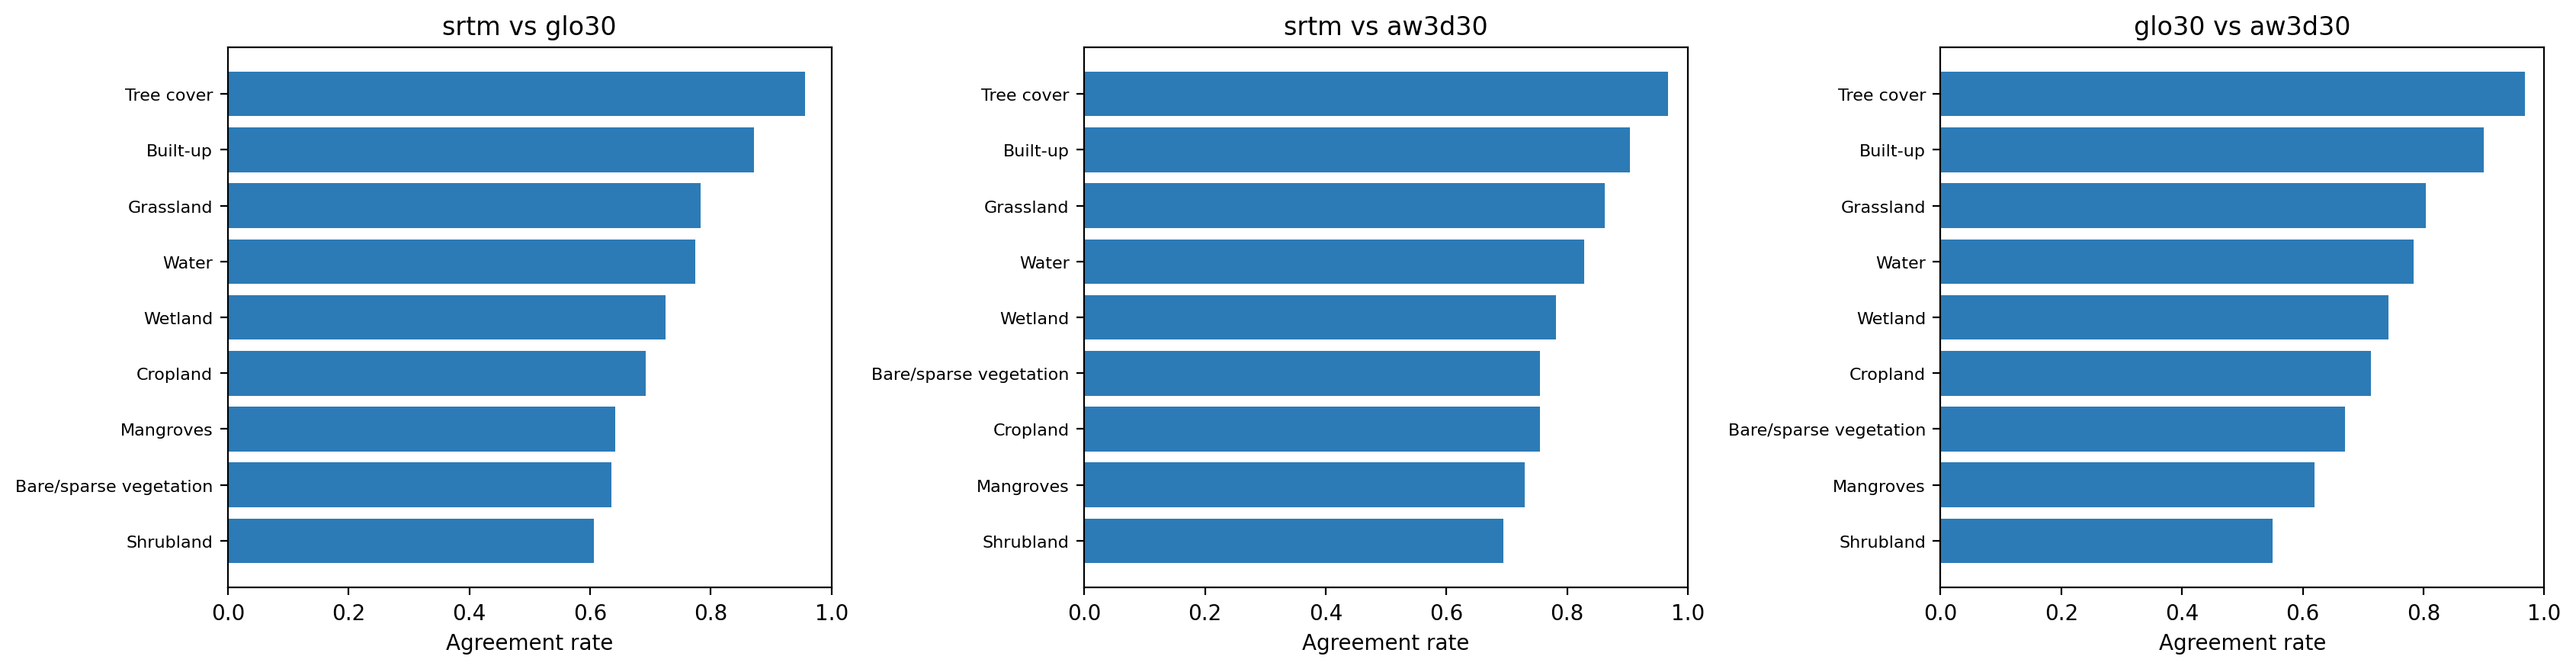
\includegraphics[width=0.92\textwidth,height=0.38\textheight,keepaspectratio]{figures/fig_agreement.png}
\caption[Stratifikasi sensitivitas spasial berdasarkan kelas WorldCover]{Stratifikasi sensitivitas spasial berdasarkan kelas tutupan lahan ESA WorldCover: (a) tingkat kesesuaian kelas (\textit{spatial agreement}, \%), dan (b) rerata selisih probabilitas absolut $\overline{|\Delta p|}$.}
\label{fig:agreement}
\end{figure}

\subsection{Analisis Autokorelasi Spasial}

Sesuai prosedur pada Subbab~3.8.1, autokorelasi spasial dilaporkan terpisah
untuk titik sampel OOF (probabilitas dan residual) dan raster peta
probabilitas karena unit analisis dan tafsirnya berbeda.

\subsubsection{Autokorelasi Spasial pada Titik Sampel}

Hasil pengujian pada titik sampel merangkum label banjir sebagai acuan,
probabilitas OOF, dan residual OOF untuk ketiga konfigurasi DEM, sebagaimana
disajikan pada Tabel~\ref{tab:moran-oof}.

\begin{table}[!htbp]
\small
\centering
\caption[Hasil Global Moran's I pada titik sampel]{Hasil Global Moran's I pada titik sampel ($n=5.956$, KNN $k=8$,
$B=9.999$, $E[I]=-0{,}000168$).}
\label{tab:moran-oof}
\begin{tabular}{llccc}
\toprule
\textbf{Variabel} & \textbf{DEM} & \textbf{$I$} & \textbf{$z$ permutasi} & \textbf{$p$ dua sisi} \\
\midrule
Label banjir (acuan) & --     & 0,677 & 109,7 & 0,0001 \\
Probabilitas OOF     & SRTM   & 0,886 & 143,6 & 0,0001 \\
Probabilitas OOF     & GLO-30 & 0,877 & 142,9 & 0,0001 \\
Probabilitas OOF     & AW3D30 & 0,882 & 142,9 & 0,0001 \\
Residual OOF         & SRTM   & 0,377 & 61,4  & 0,0001 \\
Residual OOF         & GLO-30 & 0,355 & 57,9  & 0,0001 \\
Residual OOF         & AW3D30 & 0,364 & 59,1  & 0,0001 \\
\bottomrule
\end{tabular}
\end{table}

Nilai $p=0{,}0001$ adalah batas resolusi uji permutasi (tidak ada permutasi
yang lebih ekstrem dari nilai amatan), bukan nilai $p$ yang tepat.

Probabilitas OOF pada ketiga DEM memiliki Moran's I yang tinggi (0,877 sampai
0,886) dan signifikan pada $\alpha=0{,}05$ ($p<\alpha$, tolak $H_0$). Hasil
ini wajar karena probabilitas dihasilkan dari prediktor yang berubah halus di
ruang, dan menunjukkan bahwa peta kerawanan yang dihasilkan membentuk
kelompok spasial yang koheren, bukan pola acak.

Informasi yang lebih relevan bagi evaluasi model ada pada residual OOF.
Moran's I residual bernilai positif dan signifikan pada ketiga DEM (0,355
sampai 0,377), sehingga $H_0$ ditolak. Artinya galat prediksi pada lokasi
yang berdekatan cenderung searah, dan masih ada struktur spasial yang tidak
ditangkap model, misalnya akibat proses hidrologi lokal yang tidak diwakili
prediktor. Sebagai pembanding, label banjir sendiri memiliki Moran's I 0,677,
sehingga autokorelasi residual kira-kira separuh dari autokorelasi label
(sekitar 52 persen sampai 56 persen), yang berarti model menyerap sebagian,
tetapi tidak seluruh, struktur spasial tersebut. Implikasi praktisnya adalah
bahwa amatan galat tidak independen, sehingga selang kepercayaan yang
mengandalkan resampling titik secara bebas cenderung terlalu sempit. Temuan
ini mendukung pemakaian \textit{block bootstrap} pada perbandingan AUC
antar-DEM.

Di antara ketiga DEM, residual GLO-30 memiliki Moran's I terendah (0,355),
disusul AW3D30 (0,364) dan SRTM (0,377). Urutan ini sama pada $k=5$ dan
$k=12$, dan sejalan dengan urutan AUC. Namun selisihnya kecil, tidak diuji
secara inferensial, dan nilai $I$ turun bersama kenaikan $k$ pada ketiganya,
sehingga urutan ini hanya dibaca sebagai konsistensi arah, bukan bukti
keunggulan satu DEM. Nilai Moran's I residual OOF pada uji kepekaan disajikan
pada Tabel~\ref{tab:moran-kek}.

\begin{table}[!htbp]
\small
\centering
\caption[Uji kepekaan bobot spasial Moran's I residual OOF]{Uji kepekaan bobot spasial: Moran's I residual OOF pada $k=5$, $8$,
dan $12$ ($n=5.956$).}
\label{tab:moran-kek}
\begin{tabular}{lccc}
\toprule
\textbf{DEM} & \textbf{$k=5$} & \textbf{$k=8$} & \textbf{$k=12$} \\
\midrule
SRTM   & 0,418 & 0,377 & 0,345 \\
GLO-30 & 0,393 & 0,355 & 0,326 \\
AW3D30 & 0,405 & 0,364 & 0,334 \\
\bottomrule
\end{tabular}
\end{table}

Hasil ini tidak boleh dibaca sebagai bukti bahwa \textit{spatial
cross-validation} bebas dari \textit{leakage} atau sebaliknya. Sekitar 4,4
persen pasangan tetangga ($k=8$) berada pada \textit{fold} yang berbeda.
Angka ini deskriptif dan tidak menyatakan besar \textit{leakage}. Probabilitas
OOF tiap \textit{fold} juga berasal dari model yang berbeda, sehingga
diskontinuitas di batas \textit{fold} dapat ikut memengaruhi nilai $I$.

\subsubsection{Autokorelasi Spasial pada Peta Probabilitas}

Moran's I dihitung pula pada raster probabilitas kerawanan dari model Google
Earth Engine. Bobot spasial menggunakan \textit{queen contiguity} delapan
tetangga yang distandardisasi per baris pada grid yang sama untuk ketiga DEM.
Piksel valid tanpa tetangga valid tidak disertakan. Hasil disajikan pada
Tabel~\ref{tab:moran-raster}. Angka ini merujuk pada CSV aktif dan output notebook
v28 yang telah tersinkronisasi pasca-masking AOI. Ketiga raster memakai
EPSG:32749, resolusi 30~m, dimensi $2074\times1592$, transformasi affine
seragam, serta nilai NoData $-9999$ pada sel termask. Verifikasi poligon
batas independen (\texttt{FAO/GAUL/2015/level2} Kabupaten Demak dan Kota
Semarang, luas geodesik $1.310{,}09\text{ km}^2$) terhadap ke-13 GeoTIFF
aktif mengonfirmasi bahwa seluruh piksel valid berada di dalam AOI dengan 0
piksel melampaui batas melebihi satu piksel ($30$~m; jarak pusat maksimum
piksel tepi adalah $5{,}56$~m).

\begin{table}[!htbp]
\small
\centering
\caption[Hasil Global Moran's I pada raster probabilitas]{Hasil Global Moran's I pada raster probabilitas (\textit{queen
contiguity} delapan tetangga, \textit{row-standardized}; $B=999$, \textit{seed}~42).}
\label{tab:moran-raster}
\begin{tabular}{lcccc}
\toprule
\textbf{DEM} & \textbf{Piksel valid} & \textbf{$I$} & \textbf{$E[I]$} & \textbf{$p$ dua sisi} \\
\midrule
SRTM   & 1.444.085 & 0,957714 & $-6{,}9248 \times 10^{-7}$ & 0,001 \\
GLO-30 & 1.444.085 & 0,953076 & $-6{,}9248 \times 10^{-7}$ & 0,001 \\
AW3D30 & 1.429.580 & 0,954422 & $-6{,}9951 \times 10^{-7}$ & 0,001 \\
\bottomrule
\end{tabular}
\end{table}

Hasil pada raster probabilitas menunjukkan nilai Moran's I sebesar 0,9577
pada SRTM, 0,9531 pada Copernicus DEM GLO-30, dan 0,9544 pada ALOS AW3D30.
Seluruh hasil memiliki $p$-value sebesar $0{,}001$, yaitu batas minimum
resolusi pengujian dengan $B=999$ permutasi, sehingga tidak dapat dibaca
sebagai probabilitas yang lebih kecil dari nilai tersebut.

Nilai Moran's I yang mendekati satu menunjukkan bahwa piksel-piksel yang
berdekatan cenderung memiliki nilai probabilitas kerawanan yang serupa. Pola
ini konsisten dengan sifat permukaan geografis yang berubah secara kontinu
dan menunjukkan adanya pengelompokan spasial yang kuat pada ketiga peta
probabilitas.

Moran's I raster tidak dapat dibandingkan secara numerik dengan Moran's I
titik OOF karena unit analisis dan definisi bobot spasial berbeda. Raster
merupakan keluaran model yang dilatih pada seluruh sampel, bukan prediksi OOF.
Karena itu, probabilitas OOF menggambarkan koherensi spasial pada titik yang
tidak dilihat model, residual OOF menggambarkan struktur galat yang belum
terjelaskan, dan raster menggambarkan permukaan prediksi penuh. Ketiganya
ditafsirkan secara terpisah.

\subsection{Pembahasan}
\label{ssec:pembahasan}
\enlargethispage{\baselineskip}

Hasil penelitian ini menjawab keempat rumusan masalah sebagai berikut.
Pertama, dari
aspek karakteristik parameter topografi (Rumusan Masalah~1), SRTM, Copernicus
DEM GLO-30, dan ALOS AW3D30 menghasilkan representasi bentang lahan makro yang
sejalan pada wilayah pesisir Semarang--Demak, namun memiliki perbedaan
sistematis pada elevasi median di dataran rendah pesisir serta variasi
kemiringan lereng lokal. Kontribusi karakteristik sensor dan acuan tinggi
terhadap perbedaan tersebut belum dipisahkan. Kedua, dari aspek pemodelan \textit{flood
susceptibility} berbasis Random Forest (Rumusan Masalah~2), ketiga sumber
produk elevasi menghasilkan peta kerawanan pada jalur GEE, sedangkan
evaluasi scikit-learn menunjukkan diskriminasi terhadap label proksi
pada skema \textit{holdout} acak
(ROC-AUC $0{,}932$--$0{,}940$) maupun validasi silang spasial 4-\textit{fold}
(ROC-AUC $0{,}870$--$0{,}890$).

Ketiga, dari aspek sensitivitas performa dan spasial (Rumusan Masalah~3),
pergantian sumber produk elevasi memengaruhi kinerja prediktif
sekaligus mengubah distribusi spasial kelas kerawanan banjir. Pada tingkat
performa, Copernicus DEM GLO-30 menempati peringkat tertinggi di atas ALOS
AW3D30 dan SRTM pada kelima pengujian \textit{seed}. Berdasarkan pengujian
\textit{block bootstrap}, keunggulan Copernicus DEM GLO-30 terhadap ALOS
AW3D30 ($\Delta\text{AUC}_{\text{GLO-30}-\text{AW3D30}} = +0{,}0108$
$[+0{,}0041;\,+0{,}0198]$) dan terhadap SRTM
($\Delta\text{AUC}_{\text{SRTM}-\text{GLO-30}} = -0{,}0155$
$[-0{,}0250;\,-0{,}0072]$) konsisten pada sampel ulang blok karena kedua
selang kepercayaan tidak memuat nilai nol, meskipun besaran selisihnya kecil
(maksimal sekitar $0{,}016$). Sebaliknya, selang kepercayaan untuk pasangan
SRTM dan ALOS AW3D30 memuat nilai nol, sehingga peringkat keduanya belum
dapat dipisahkan pada skema ini. Pada tingkat spasial, kesesuaian kelas
antarpeta berkisar antara 79,4\% dan 84,3\%, sementara pergeseran luas kedua
kelas kerawanan ekstrem terhadap SRTM sebagai peta acuan berkisar dari
penyempitan sekitar 4,6\% pada ALOS AW3D30 hingga pelebaran sekitar 9\%
pada Copernicus DEM GLO-30. Perbedaan tersebut terkonsentrasi pada kelas ekstrem dan
menunjukkan bahwa selisih metrik evaluasi yang tampak kecil pada tingkat
model tetap dapat menghasilkan perbedaan delineasi spasial yang dapat
menjadi pertimbangan dalam interpretasi hasil pemetaan kerawanan banjir.
Keempat, dari aspek stratifikasi tutupan lahan
(Rumusan Masalah~4), sensitivitas spasial tertinggi terjadi pada tutupan
semak belukar (\textit{shrubland}, kesesuaian kelas 57,6\%--75,4\%), lahan
terbuka atau vegetasi jarang (\textit{bare/sparse vegetation},
63,1\%--78,1\%), serta kawasan mangrove (62,6\%--74,9\%), sedangkan tutupan
pohon dan kawasan terbangun relatif lebih stabil. Temuan ini sejalan dengan
kajian Meadows dkk.\ \citep{meadows2024} yang menunjukkan bahwa variasi
galat produk elevasi global berkaitan dengan kondisi tutupan permukaan dan
karakteristik morfologi setempat.

\enlargethispage{\baselineskip}Di luar keempat rumusan masalah utama tersebut, eksperimen ini juga mengungkap
temuan metodologis tambahan mengenai tingginya kepekaan estimasi kinerja model
terhadap desain pengambilan sampel kelas non-banjir. Pergeseran
domain sampel non-banjir dari zona sekitar perairan permanen menuju seluruh
wilayah kajian disertai perbedaan ROC-AUC validasi silang spasial dari sekitar
$0{,}70$ menjadi $0{,}870$ hingga $0{,}890$ ($\Delta\text{AUC} \approx
0{,}17$) dibandingkan selisih antarproduk elevasi
($\Delta\text{AUC} \approx 0{,}01$). Kedua angka ini berasal dari domain
sampel yang berbeda, sehingga perbandingannya bersifat deskriptif dan tidak
mengisolasi pengaruh domain atau satu komponen desain tertentu. Meskipun
\textit{block bootstrap} dan pengujian multi-\textit{seed} mendukung keunggulan
Copernicus DEM GLO-30 pada eksperimen ini, hasil tersebut tidak dimaksudkan
untuk menetapkan satu produk elevasi sebagai pilihan terbaik di seluruh
wilayah atau kejadian banjir lain.

Eksperimen mencakup satu periode kejadian banjir pada satu wilayah kajian dan
menggunakan satu \textit{seed} utama untuk pembuatan peta. Kestabilan metrik
telah diuji pada lima \textit{seed}. Karena itu, hasil ini belum menggambarkan
perilaku model pada kejadian banjir atau wilayah lain.

Dari sisi konstruksi label, \textit{flood inventory} Sentinel-1 yang digunakan
merupakan label proksi pengamatan, bukan data pengamatan lapangan
(\textit{ground truth}) yang independen. Konsekuensinya sejalan dengan
definisi pada Subbab~2.2 dan prosedur pada
Subbab~\ref{ssec:flood-inventory}: label kelas~1 menyatakan piksel yang terdeteksi
banjir oleh pipeline proksi, sedangkan label kelas~0 menyatakan piksel yang
tidak diidentifikasi banjir oleh pipeline yang sama dan bukan bukti lokasi
tersebut tidak berbanjir. Besaran \textit{false negative} pada kelas~0 tidak
terkuantifikasi dalam eksperimen ini. Label juga tidak sepenuhnya
independen terhadap salah satu produk perlakuan karena penyaringan kemiringan
lereng menggunakan SRTM, sementara penyaringan perairan permanen memanfaatkan
pita JRC Global Surface Water yang cakupannya terbatas (masker mencakup
sekitar 12,8\%--14,4\% wilayah kajian dan nilai \textit{occurrence} terbaca
pada sekitar 4,3\% wilayah kajian), sehingga label positif hanya dapat
terbentuk di dalam area dukungan tersebut, sedangkan kandidat kelas~0
mencakup area di dalam dan di luarnya. Kecocokan label hasil ekstraksi
ulang dilaporkan sebesar 70\% terhadap 1.870 titik penelitian acuan.
Perbedaan ini belum dapat diatribusikan hanya pada pembaruan arsip
Sentinel-1. Karena himpunan label yang sama diterapkan identik
pada ketiga konfigurasi, kesetaraan perlakuan antarproduk elevasi tetap
terjaga, namun kesetaraan pengolahan tersebut tidak menghilangkan seluruh
sumber bias label. Dengan demikian, hasil evaluasi perlu ditafsirkan sebagai
kemampuan model mereproduksi label proksi tersebut, bukan sebagai ukuran
akurasi terhadap seluruh kejadian banjir aktual di lapangan. Di luar
dukungan label positif JRC, prediksi berasal dari model yang dapat menerima
sampel kelas~0 dari area tersebut tetapi tidak memiliki contoh positif
setempat. Prediksi ini tidak membuktikan keberadaan atau ketiadaan banjir
aktual di luar dukungan label positif.
Terdapat pula perbedaan sifat representasi permukaan antara SRTM yang
berbasis radar pita-C dan Copernicus DEM GLO-30 serta ALOS AW3D30 yang
berkarakteristik \textit{Digital Surface Model} (DSM), ditambah perbedaan
acuan tinggi (EGM96 pada SRTM dan ALOS AW3D30, EGM2008 pada Copernicus
DEM GLO-30) yang dilaporkan tanpa koreksi geoid.

\enlargethispage{\baselineskip}Batasan yang memengaruhi interpretasi juga bersumber dari prediktor. Prediktor
hidrologi berasal dari MERIT Hydro, yakni turunan produk elevasi di luar
ketiga perlakuan, sehingga variabel tersebut memuat muatan topografi yang
tidak berubah antarperlakuan dan kaitannya dengan karakteristik masing-masing
DEM bersifat tidak langsung. Prediktor terkait air seperti NDWI, MNDWI, dan
jarak ke badan air menangkap informasi yang sebagian tumpang tindih dengan
definisi label berbasis Sentinel-1, sehingga tingkat probabilitas absolut
pada masing-masing peta perlu dibaca dengan hati-hati meskipun perbandingan
antarproduk memakai label yang sama.

Granularitas evaluasi spasial masih terbatas pada 16 blok kuantil, dan
implementasi pemodelan dilakukan pada dua lingkungan dengan konfigurasi
serumpun, yaitu peta dengan 300 pohon pada Google Earth Engine serta metrik
evaluasi dengan 400 pohon pada scikit-learn. Statistik spasial raster
berasal dari peta Google Earth Engine, sedangkan statistik titik OOF dan
metrik performa berasal dari evaluasi scikit-learn. Keterbatasan tersebut
menjadi dasar bagi arah pengembangan yang
diuraikan pada Subbab~5.2.

Analisis diagnostik autokorelasi spasial membawa keterbatasan yang
perlu dicatat. \textit{Spatial cross-validation} memakai 16 blok bersebelahan
tanpa zona penyangga, sehingga titik di tepi blok dapat berdekatan dengan
data latih. Kebocoran berkurang tetapi tidak dapat dinyatakan hilang. Global
Moran's I adalah analisis diagnostik: hasilnya tidak membuktikan ada atau
tidaknya \textit{spatial leakage}, dan hasil yang tidak signifikan tidak
menunjukkan ketiadaan autokorelasi. Nilai Moran's I juga bergantung pada
definisi bobot spasial. Uji kepekaan dilakukan untuk $k=5$, $8$, dan $12$,
tetapi definisi lain (misalnya pita jarak) tidak diuji.

Probabilitas OOF tiap \textit{fold} berasal dari model berbeda, dan Moran's I
hanya dianalisis pada evaluasi utama, bukan pada dataset multi-\textit{seed}.
Uji permutasi mengasumsikan keterpertukaran nilai di bawah $H_0$, yang dapat
dilanggar jika residual bersifat heteroskedastis. Perbedaan Moran's I
antar-DEM tidak diuji secara inferensial.

\FloatBarrier

\clearpage

%==================================================================
% BAB V
%==================================================================

\bab{Kesimpulan dan Saran}

\subsection{Kesimpulan}

Berdasarkan hasil pemodelan pada Bab~IV, berikut dirangkum jawaban atas
keempat pertanyaan rumusan masalah pada Subbab~1.2:

\begin{enumerate}
\item Karakteristik SRTM, Copernicus DEM GLO-30, dan ALOS AW3D30 terbawa
ke dalam parameter topografi yang dihitung dari masing-masing produk:
perbedaan antarproduk dilaporkan secara deskriptif dan spasial pada elevasi
serta kemiringan lereng, termasuk nilai median elevasi dan offset vertikal
antarproduk (Subbab~4.1). Arah lereng masuk sebagai prediktor melalui
dekomposisi sinus--kosinus beserta indikator validitasnya, tanpa ringkasan
numerik lintasproduk yang dilaporkan tersendiri.
\item Ketiga peta probabilitas kerawanan banjir dihasilkan menggunakan sampel,
label, dan konfigurasi pemodelan yang dipertahankan sama, dengan lima
prediktor turunan DEM yang disesuaikan menurut produk elevasi yang digunakan.
Perbedaan hasil antarpeta kemudian dianalisis sebagai sensitivitas terhadap
pergantian sumber elevasi dalam kerangka eksperimen terkontrol. Ketiga peta
menunjukkan tingkat kesesuaian kelas sebesar 79,4\% hingga 84,3\%.
Meskipun sebagian besar piksel memiliki kelas kerawanan yang sama,
pergantian sumber elevasi tetap menghasilkan perubahan distribusi spasial,
terutama pada kelas kerawanan ekstrem, yaitu sangat rendah dan sangat tinggi
(Subbab~4.3 dan Subbab~4.5).
\item Pergantian sumber elevasi menghasilkan perbedaan kinerja yang kecil
tetapi konsisten: keunggulan Copernicus DEM GLO-30 terhadap ALOS AW3D30 dan
terhadap SRTM konsisten pada sampel ulang blok (Subbab~4.4), sedangkan
selang kepercayaan untuk pasangan SRTM dan ALOS AW3D30 masih memuat nol
sehingga peringkat keduanya belum dapat dipisahkan. Risiko ketergantungan
spasial diperhatikan melalui validasi silang spasial dan \textit{block bootstrap}
(Subbab~3.8). Namun, Moran's I residual OOF masih bernilai positif dan
signifikan pada ketiga DEM (0,355 sampai 0,377). Dengan demikian, rancangan
evaluasi ini belum dapat dianggap sepenuhnya menghilangkan ketergantungan
spasial. Prosedur \textit{block bootstrap} tetap menjadi analisis utama perbandingan
antarproduk.
Autokorelasi positif pada probabilitas OOF (0,877 sampai 0,886) dan pada label
acuan (0,677) menunjukkan struktur spasial data yang sebagian serap model,
dengan rancangan 16 blok mengurangi risiko kebocoran spasial meskipun belum
dapat dinyatakan telah menghilangkan kebocoran tersebut (Subbab~4.7).
\item Sensitivitas spasial tidak seragam antar kelas tutupan lahan ESA
WorldCover: kelas tutupan pohon paling stabil, diikuti kawasan terbangun,
sedangkan sensitivitas tertinggi terkonsentrasi pada semak belukar, lahan
terbuka atau vegetasi jarang, serta mangrove (Subbab~4.6).
\end{enumerate}

\subsection{Saran}

Berdasarkan hasil dan keterbatasan penelitian, saran yang diajukan adalah
sebagai berikut:

\begin{enumerate}
\item Perluasan cakupan kejadian banjir pada \textit{flood inventory} agar
sensitivitas sumber elevasi dievaluasi pada kondisi banjir yang lebih
representatif.
\item Peningkatan granularitas blok evaluasi spasial (blok lebih banyak dari
16 blok kuantil) untuk mengukur sensitivitas hasil terhadap pilihan skema
blok.
\item Penambahan evaluasi ketidakpastian \textit{flood inventory}, khususnya
terhadap variabilitas arsip Sentinel-1 dan cakupan pita JRC yang telah
dilaporkan sebagai batasan.
\item Penggunaan hasil sensitivitas sebagai bahan pertimbangan pemilihan
produk elevasi terbuka bagi pemetaan kerawanan banjir wilayah pesisir lain
yang menghadapi keterbatasan data topografi beresolusi tinggi.
\end{enumerate}

\FloatBarrier

\clearpage

\clearpage
\phantomsection
\addcontentsline{toc}{section}{DAFTAR PUSTAKA}
\thispagestyle{plain}
{\centering\large\bfseries DAFTAR PUSTAKA\par}
\vspace{1.5em}
\begingroup
\singlespacing
\renewcommand{\section}[2]{}
\setlength{\bibhang}{2em}
\setlength{\bibsep}{0.65em}
\begin{thebibliography}{99}
\bibitem[Abidin et al.(2013)]{abidin2015} Abidin, H.~Z., Andreas, H., Gumilar, I., Sidiq, T.~P., dan Fukuda, Y. 2013. Land subsidence in coastal city of Semarang (Indonesia): Characteristics, impacts and causes. \textit{Geomatics, Natural Hazards and Risk}, 4(3):226--240.

\bibitem[Breiman(2001)]{breiman2001} Breiman, L. 2001. Random forests. \textit{Machine Learning}, 45(1):5--32.

\bibitem[ESA(2021)]{esa_glo30} European Space Agency. 2021. \textit{Copernicus Digital Elevation Model (DEM) GLO-30}. Dataset, Copernicus Contributing Missions. DOI: 10.5270/ESA-c5d3d65.

\bibitem[Farr et al.(2007)]{farr2007} Farr, T.~G., Rosen, P.~A., Caro, E., Crippen, R., Duren, R., Hensley, S., Kobrick, M., Paller, M., Rodriguez, E., Roth, L., Seal, D., Shaffer, S., Shimada, J., Umland, J., Werner, M., Oskin, M., Burbank, D., dan Alsdorf, D. 2007. The Shuttle Radar Topography Mission. \textit{Reviews of Geophysics}, 45(2):RG2004.

\bibitem[Fatdillah et al.(2022)]{fatdillah2022} Fatdillah, E., Rehan, B.~M., Rameshwaran, P., Bell, V.~A., Zulkafli, Z., Yusuf, B., dan Sayers, P. 2022. Spatial estimates of flood damage and risk are influenced by the underpinning DEM resolution: A case study in Kuala Lumpur, Malaysia. \textit{Water}, 14(14):2208.

\bibitem[Fereshtehpour et al.(2024)]{fereshtehpour2024} Fereshtehpour, M., Esmaeilzadeh, M., Alipour, R.~S., dan Burian, S.~J. 2024. Impacts of DEM type and resolution on deep learning-based flood inundation mapping. \textit{Earth Science Informatics}, 17(2):1125--1145.

\bibitem[Fikri et al.(2026)]{fikri2026} Fikri, R.~M., Herawati, H., dan Pranoto, W.~A. 2026. Influence of DEM spatial resolution on the accuracy and computational efficiency of HEC-RAS 1D and 2D flood inundation modelling: A case study of the Cimanceuri Basin, Indonesia. \textit{Water}, 18(10):1203.

\bibitem[Funk et al.(2015)]{funk2015} Funk, C., Peterson, P., Landsfeld, M., Pedreros, D., Verdin, J., Shukla, S., Husak, G., Rowland, J., Harrison, L., Hoell, A., dan Michaelsen, J. 2015. The climate hazards infrared precipitation with stations---a new environmental record for monitoring extremes. \textit{Scientific Data}, 2(1):150066.

\bibitem[Gorelick et al.(2017)]{gorelick2017} Gorelick, N., Hancher, M., Dixon, M., Ilyushchenko, S., Thau, D., dan Moore, R. 2017. Google Earth Engine: Planetary-scale geospatial analysis for everyone. \textit{Remote Sensing of Environment}, 202:18--27.

\bibitem[Hakim et al.(2026)]{hakim2026} Hakim, M.~I.~A., Fann, A.~G.~Z., dan Kharisudin, I. 2026. Comparative explainable ensemble learning for flood susceptibility mapping using Sentinel-1-derived flood inventory and multi-source geospatial data: A case study of the Semarang-Demak coastal area. \textit{Statistical Modeling and Data Science}, 1(1):22--47.

\bibitem[Husnayaen et al.(2018)]{Husnayaen2018} Husnayaen, Rimba, A.~B., Osawa, T., Parwata, I.~N.~S., As-syakur, A.~R., Kasim, F., dan Astarini, I.~A. 2018. Physical assessment of coastal vulnerability under enhanced land subsidence in Semarang, Indonesia, using multi-sensor satellite data. \textit{Advances in Space Research}, 61(8):2159--2179.

\bibitem[Islam dan Meng(2022)]{islammeng2022} Islam, M.~T. dan Meng, Q. 2022. An exploratory study of Sentinel-1 SAR for rapid urban flood mapping on Google Earth Engine. \textit{International Journal of Applied Earth Observation and Geoinformation}, 113:103002.

\bibitem[Marfai dan King(2008)]{marfai2008} Marfai, M.~A. dan King, L. 2008. Potential vulnerability implications of coastal inundation due to sea level rise for the coastal zone of Semarang City, Indonesia. \textit{Environmental Geology}, 54(6):1235--1245.

\bibitem[Meadows et al.(2024)]{meadows2024} Meadows, M., Jones, S., dan Reinke, K. 2024. Vertical accuracy assessment of freely available global DEMs (FABDEM, Copernicus DEM, NASADEM, AW3D30 and SRTM) in flood-prone environments. \textit{International Journal of Digital Earth}, 17(1):2308734.

\bibitem[Moran(1950)]{moran1950} Moran, P.~A.~P. 1950. Notes on continuous stochastic phenomena. \textit{Biometrika}, 37(1/2):17--23.

\bibitem[Pekel et al.(2016)]{pekel2016} Pekel, J.-F., Cottam, A., Gorelick, N., dan Belward, A.~S. 2016. High-resolution mapping of global surface water and its long-term changes. \textit{Nature}, 540(7633):418--422.

\bibitem[Ploton et al.(2020)]{ploton2020} Ploton, P., Mortier, F., R{\'e}jou-M{\'e}chain, M., Barbier, N., Picard, N., Rossi, V., Dormann, C., Cornu, G., Viennois, G., Bayol, N., Lyapustin, A., Gourlet-Fleury, S., dan P{\'e}lissier, R. 2020. Spatial validation reveals poor predictive performance of large-scale ecological mapping models. \textit{Nature Communications}, 11:4540.

\bibitem[Roberts et al.(2017)]{roberts2017} Roberts, D.~R., Bahn, V., Ciuti, S., Boyce, M.~S., Elith, J., Guillera-Arroita, G., Hauenstein, S., Lahoz-Monfort, J.~J., Schröder, B., Thuiller, W., Warton, D.~I., Wintle, B.~A., Hartig, F., dan Dormann, C.~F. 2017. Cross-validation strategies for data with temporal, spatial, hierarchical, or phylogenetic structure. \textit{Ecography}, 40(8):913--929.

\bibitem[Saha et al.(2021)]{saha2021} Saha, T.~K., Pal, S., Talukdar, S., Debanshi, S., Khatun, R., Singha, P., dan Mandal, I. 2021. How far spatial resolution affects the ensemble machine learning based flood susceptibility prediction in data sparse region. \textit{Journal of Environmental Management}, 297:113344.

\bibitem[Sakina et al.(2025)]{Sakina2025} Sakina, S.~L., Ningsih, N.~S., dan Prayogi, A. 2025. Investigating wave characteristics in the Java Sea and potential influencing factors: A case study of coastal flooding along the northern coast of Semarang City, Indonesia (May 23, 2022). \textit{Anthropocene Coasts}, 8(1):44.

\bibitem[Tadono et al.(2016)]{tadono2016} Tadono, T., Nagai, H., Ishida, H., Oda, F., Naito, S., Minakawa, K., dan Iwamoto, H. 2016. Generation of the 30 m-mesh global digital surface model by ALOS PRISM. \textit{The International Archives of the Photogrammetry, Remote Sensing and Spatial Information Sciences}, XLI-B4:157--162.

\bibitem[Tique et al.(2026)]{Tique2026} Tique, W.~F.~M., Sapena, M., Weigand, M., Groth, S., Gei{\ss}, C., dan Taubenb{\"o}ck, H. 2026. A comparative assessment of data-driven flood susceptibility mapping in Nigeria. \textit{Natural Hazards}, 122(4):1--29.

\bibitem[UN-SPIDER(2024)]{unspider2024} UN-SPIDER. 2024. \textit{Recommended Practice: Flood Mapping Using Sentinel-1 Data in Google Earth Engine}. United Nations Platform for Space-based Information for Disaster Management and Emergency Response.

\bibitem[Verdyansyah et al.(2025)]{verdyansyah2025} Verdyansyah, A., Helmi, M., dan Widiaratih, R. 2025. Integrating CMIP6 and remote sensing datasets for current and future flood susceptibility projections using machine learning under climate change scenarios in Demak District for future sustainable planning. \textit{Sustainability}, 17(18):8188.

\bibitem[Yamazaki et al.(2019)]{yamazaki2019} Yamazaki, D., Ikeshima, D., Sosa, J., Bates, P.~D., Allen, G.~H., dan Pavelsky, T.~M. 2019. MERIT Hydro: A high-resolution global hydrography map based on latest topography dataset. \textit{Water Resources Research}, 55(6):5053--5073.

\bibitem[Youden(1950)]{youden1950} Youden, W.~J. 1950. Index for rating diagnostic tests. \textit{Cancer}, 3(1):32--35.

\bibitem[Yuwono et al.(2024)]{yuwono2024} Yuwono, B.~D., Awaluddin, M., dan Najib. 2024. Mapping of flood hazard induced by land subsidence in Semarang City, Indonesia, using hydraulic and spatial models. \textit{Natural Hazards}, 120(6):5333--5368.

\bibitem[Zanaga et al.(2022)]{zanaga2021} Zanaga, D., Van De Kerchove, R., Daems, D., De Keersmaecker, W., Brockmann, C., Kirches, G., Wevers, J., Cartus, O., Santoro, M., Fritz, S., Lesiv, M., Herold, M., Tsendbazar, N.-E., Xu, P., Ramoino, F., dan Arino, O. 2022. \textit{ESA WorldCover 10 m 2021 v200}. European Space Agency (ESA). DOI: 10.5281/zenodo.7254221.

\end{thebibliography}
\endgroup
\end{document}
